\chapter{Space Time}	
\label{chapterIV}
\section{Introduction}

The previous chapter shows that institutional investment is mostly an urban phenomenon.  This chapter examines the evolution of institutional investors across space and time.  Furthermore, for ease of statistical analysis, both databases will only draw from investors located in the continental United States (CONUS), as well as for the top 5 core-based statistical areas (CBSA) in terms of total institutional investment.  In alphabetical order, these 5 metro regions are Boston, Chicago, Los Angeles, New York City and San Francisco.  


\section{Space-Time Cube}

The space-time cube is a space-time analytical technique that bins point objects into a space-time grid in order to examine the relationship between points not only in space but across time \cite{Esri}. Two types of space-time cubes are created, the first one aggregates the total number of institutional investors for the time period of March 1999 to December 2018.  The second space-time cube aggregates the total number of funds under management for the period of June 2013 to December 2018.  

The first step in creating a space-time cube is the creation of a Network Common Data Form (NetCDF) file.   This file format permits ArcGIS to store multidimensional information with a defined geographical position (x and y) alongside a defined time period as well as any additional relevant information such as count data, sum, average, median and standard deviation.  This creates a data-structure in which further analysis can be performed, such as emerging hotspot analysis and local outlier analysis. Figure \ref{fig:timecube1} provides two perspectives on the data aggregation process. 

\begin{figure}
	\centering
	
	
	\begin{subfigure}[b]{0.45\textwidth}
		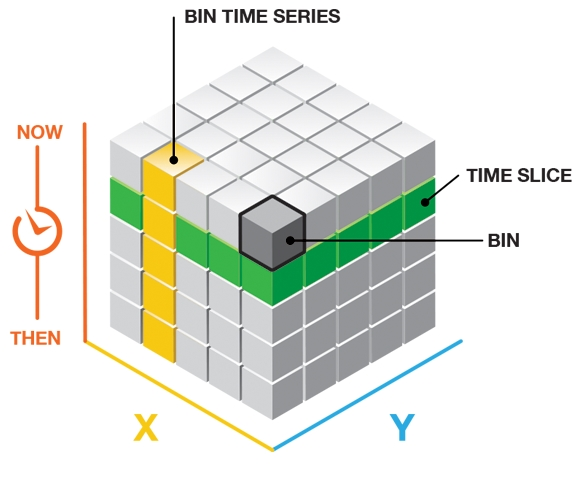
\includegraphics[width=1\linewidth]{Figures/ChapterIV/TimeCube}
		\caption{A schematic explanation of the time-cube }
		\label{fig:Timecube}
	\end{subfigure}
	\begin{subfigure}[b]{0.45\textwidth}
		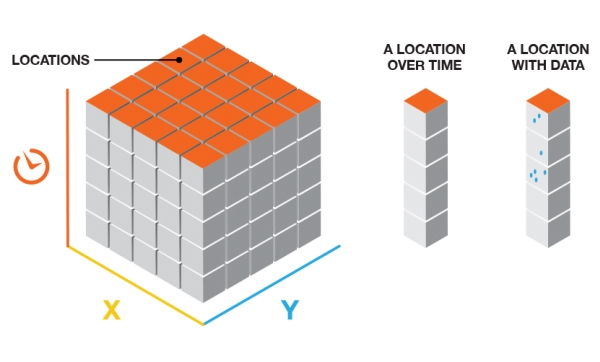
\includegraphics[width=1\linewidth]{Figures/ChapterIV/Time_Cube_Slice}
		\caption{Examination of a time-cube cell}
		\label{fig:timesclice}
	\end{subfigure}
	
	\caption[ESRI Schematic Illustrations of a Time-Cube]{Schematic illustration of a time-cube. It should be noted that unlike this schematic representation of the time-cube, the analysis in this paper uses a hexagonal bin rather than a square bin for spatial data.  Image from: \url{http://desktop.arcgis.com/en/arcmap/10.3/tools/space-time-pattern-mining-toolbox/visualizing-cube-data.htm}}
	\label{fig:timecube1}
\end{figure}


It should be noted that unlike Figure \ref{fig:Timecube} and \ref{fig:timesclice}, this analysis was run using hexagonal bins. Unlike the traditional square bins (or in Esri's parlance, a fishnet grid), the hexagons have multiple advantages over squares, such as:  of the three geometric forms that can tessellate (repeat a shape over and over without overlap), the  square, the hexagon and the equilateral triangle, hexagons have the lowest perimeter to area ratio.  This is due to hexagons being the closest of the three tessellating shapes to a circle.  As such, this reduces the border effect when binning points, since the hexagon has the shortest average distance between perimeter and centroid.  Furthermore, the centroids of hexagons are equidistant from each other when tessellated.  This cannot be said about squares in a grid using the queen's movement, for the distances between centroids in square bins are shorter along the rook's movement than the bishop's movement due the Pythagorean theorem.  Lastly, at larger distances hexagons suffer less distortion than squares.  Unfortunately for square bins, the implementation of spatial bins in this project does not play to its strengths, such as ease of use when conducting matrix algebra and having an orthogonal coordinate system \citep{birch2007rectangular}. 

With regards to the time dimension of the data, the dates are aligned such that bins coincide with the last date in the datasets (December 31, 2018) and work backwards from there in 3 month intervals.  As such, each temporal bin covers one filing period for 13F-HR disclosures.  (Figure \ref{fig:timesclice})

\subsection{Emerging hot spot analysis}

Emerging hot spot analysis is the space-time implementation of the Getis-Ord Gi* statistic \citep{getis2010analysis}, and examines whether high or low values cluster geographically.  High $g$ values are created when the local sum and that of its neighbours are significantly larger than their proportion to the global sum, with low values in the reverse case. The ArcGIS implementation of Emerging Hot Spot Analysis performs the False Discovery Rate (FDR) correction.  FDR accounts for multiple testing, and therefore compensates for the possibility that certain features would be classified as hot or cold by chance alone \citep{Esri}.

The next step is to perform Mann-Kendall trend test to detect temporal trends at each spatial location. Depending on the results of the Getis-Ord Gi* statistic and the trend direction from the Mann-Kendall test, there is a total of 17 possible answers, and their definitions are listed in Table \ref{App:EmergingHotspotdef} in Appendix \ref{Definition_appendix} \citep{Esri}.

\subsection{Local Outlier Analysis}

Local outlier analysis is the space-time implementation of the Anselin Local Moran's I statistic.  This tool identifies concentrations of high values (high-high), low values (low-low) in addition to spatial ouliers in which high values are surrounded by low values (high-low), and low values that are surrounded by high values (low-high).  Unlike traditional Anselin Local Moran's I statistic, the local outlier analysis variant offers a 5th category, in which it flags bins that have different Anselin Local Moran's I statistic values during the timeframe.  

\section{United States of America}

The first use of space-time analysis will focus on the United States as a whole, after which the basic analysis will be repeated on the five largest metro areas. 

When creating the NetCDF file for the United States of America, the size of spatial bins was set at 50 km.  This value was chosen since this permitted a local window with a radius of 300 km according to the ESRI implementations of Emerging Hotspot Analysis and Local Outlier Analysis.  This latter figure is important since it would represent the longest possible day trip during a business day \citep{Fritsch06}.  Furthermore, we should keep in mind that the 50 km range band showed one of the highest level of change over time with regards to the K-function.  

\subsection{Count Data}

Figure \ref{fig:usahspcount} shows the results of the emerging hotspot analysis using the address book database. These results should come as no surprise after reading the previous chapter, in which the vast majority of institutional investors are located in the New York, Boston, Chicago, Los Angeles and San Francisco regions.  After all, institutional investment is a decidedly urban phenomenon despite being a theoretically footloose industry in an era of wireless telecommunications and computerized stock trading.  In addition to these regions, there is some strong, but inconsistent growth in the Texas Triangle (a megaregion that encompasses San Antonio, Dallas-Fort Worth and Houston), the Miami-Dade region of South Florida, the Ohio Valley and the Raleigh Triangle (Raleigh, Durham and Chapel Hill, North Carolina).  


\begin{figure}[h]
	\centering
	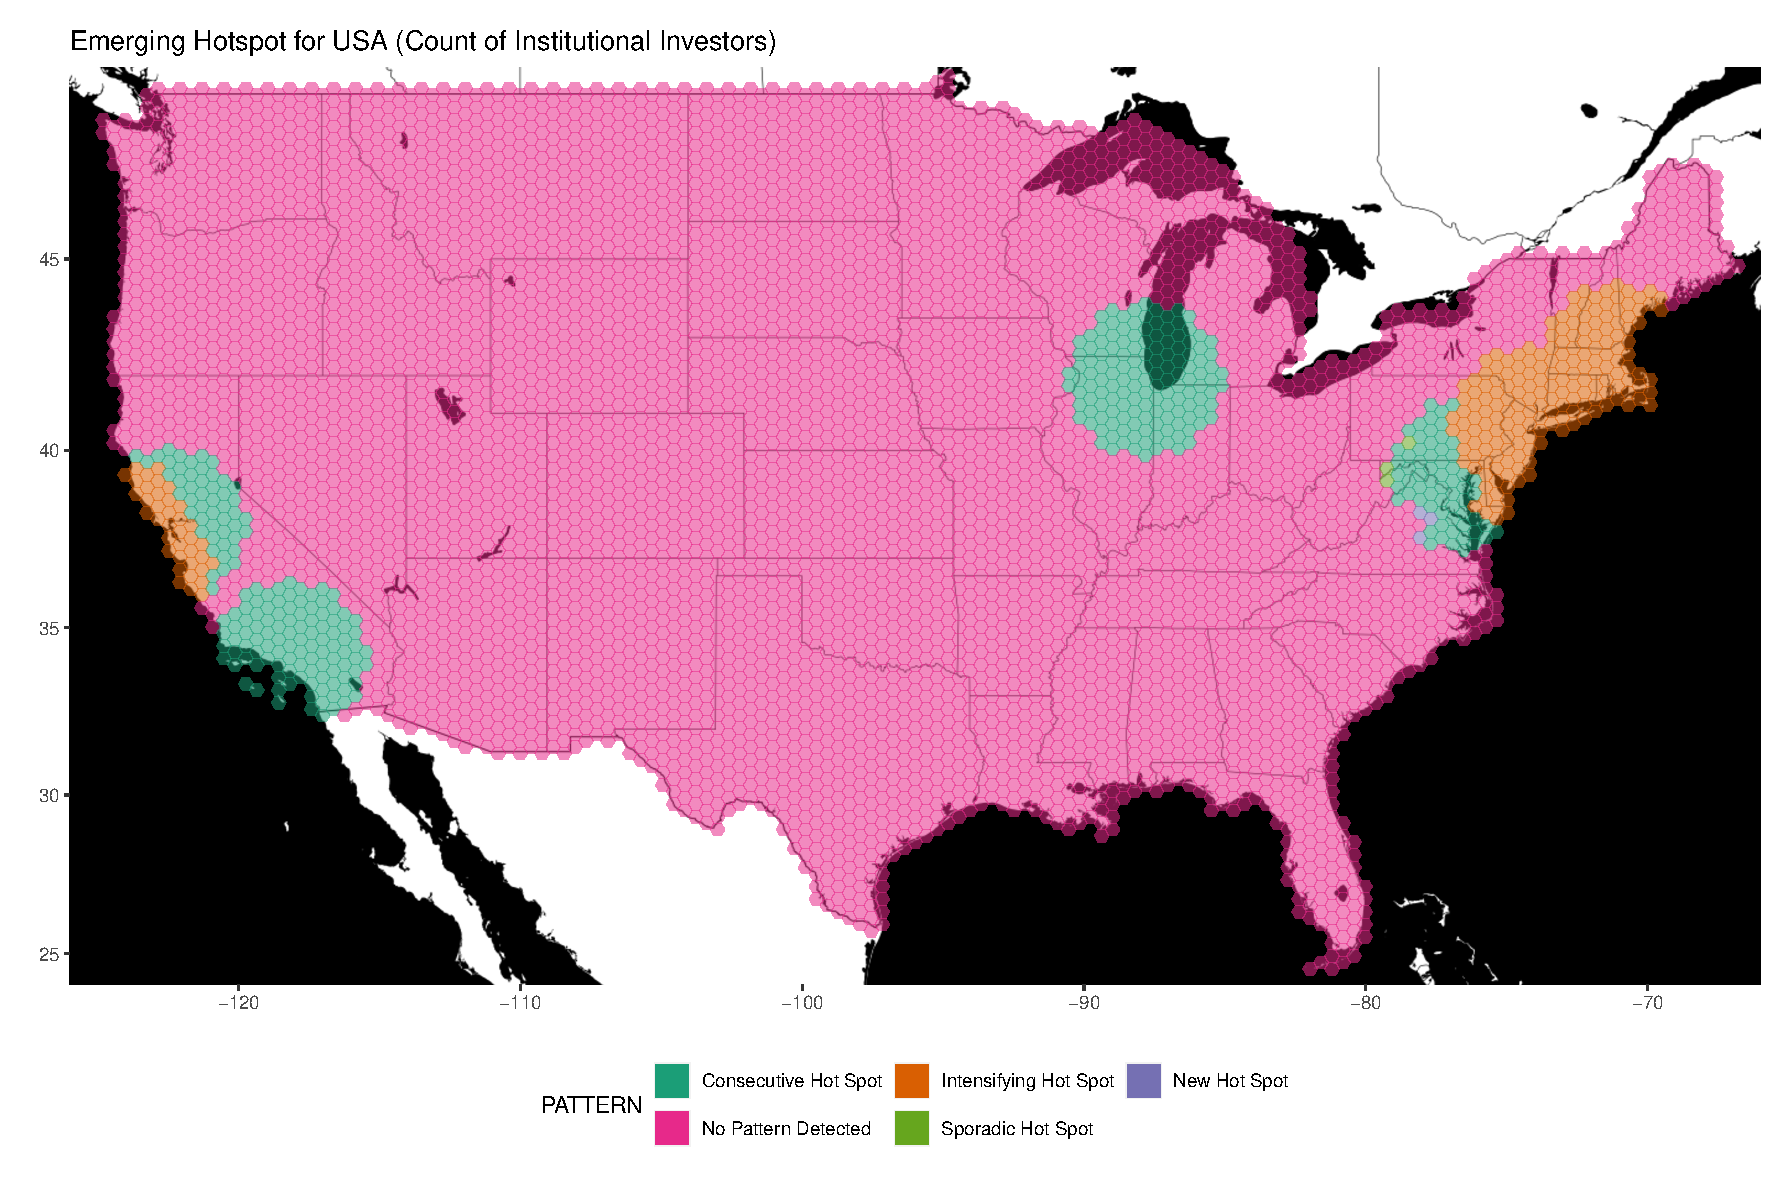
\includegraphics[width=1\linewidth]{Figures/ChapterIV/USA_Count_EH}
	\caption[Emerging Hot Spot Analysis of Locations of Institutional Investors in the USA 1999-2018]{Emerging hot spot analysis of locations of institutional investors in the United States of America for the period of March 1999 to December 2018.}
	\label{fig:usahspcount}
\end{figure}

Painting a similar picture than Figure \ref{fig:usahspcount},  the local outlier analysis (Figure \ref{fig:usaloacount}) indicates that the cities of New York, Boston, Chicago, Los Angeles and San Francisco are high-high clusters.  

What is also of interest, is the light sprinkling of high-low clusters in Figure \ref{fig:usaloacount}.  These light blue dots coincide with secondary and tertiary financial centres as well as State capitals where State-employee pension funds are managed.  
Low-high clusters appear to be confined to bridging the gaps between nearby high-high clusters, such as the peripheral areas of the North-East mega-region.  These low-high clusters are not unexpected, since they are definitionally low areas surrounded on multiple sides by high areas.     

\begin{figure}
	\centering
	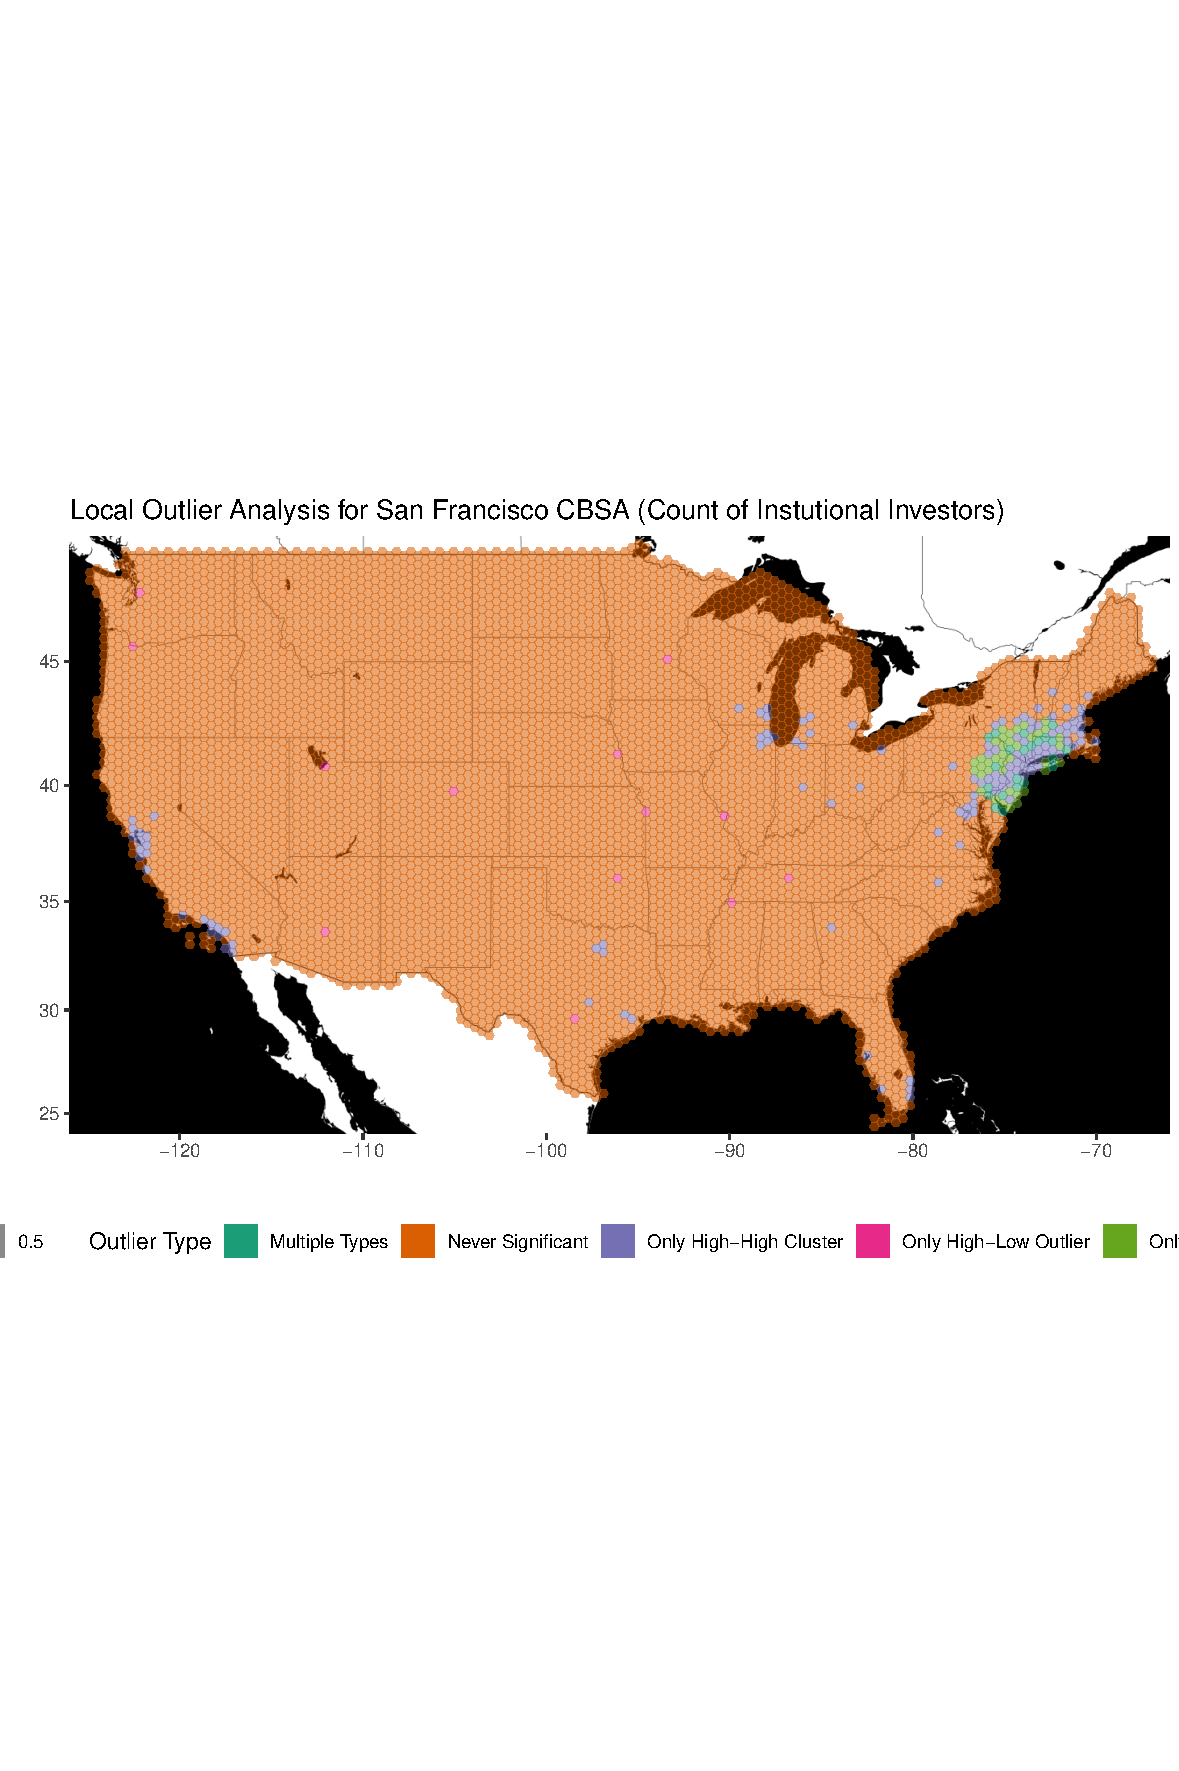
\includegraphics[width=1\linewidth]{Figures/ChapterIV/USA_Count_LO}
	\caption[Local Outlier Analysis for Number of Institutional Investors in the USA 1999-2018]{Local outlier analysis for number of institutional investors in the USA for the time period March 1999 to December 2018}
	\label{fig:usaloacount}
\end{figure}

\subsection{Funds Under Management}

Using the same technique on the holdings database presents a slightly different  outcome as seen in Figure \ref{fig:usaHSP_Money}. Using money under management rather than count data puts more emphasis on New York and San Francisco, while at the same time removing all of the consecutive cold spot areas and turning them into regions with no detectable patterns.  	

\begin{figure}
	\centering
	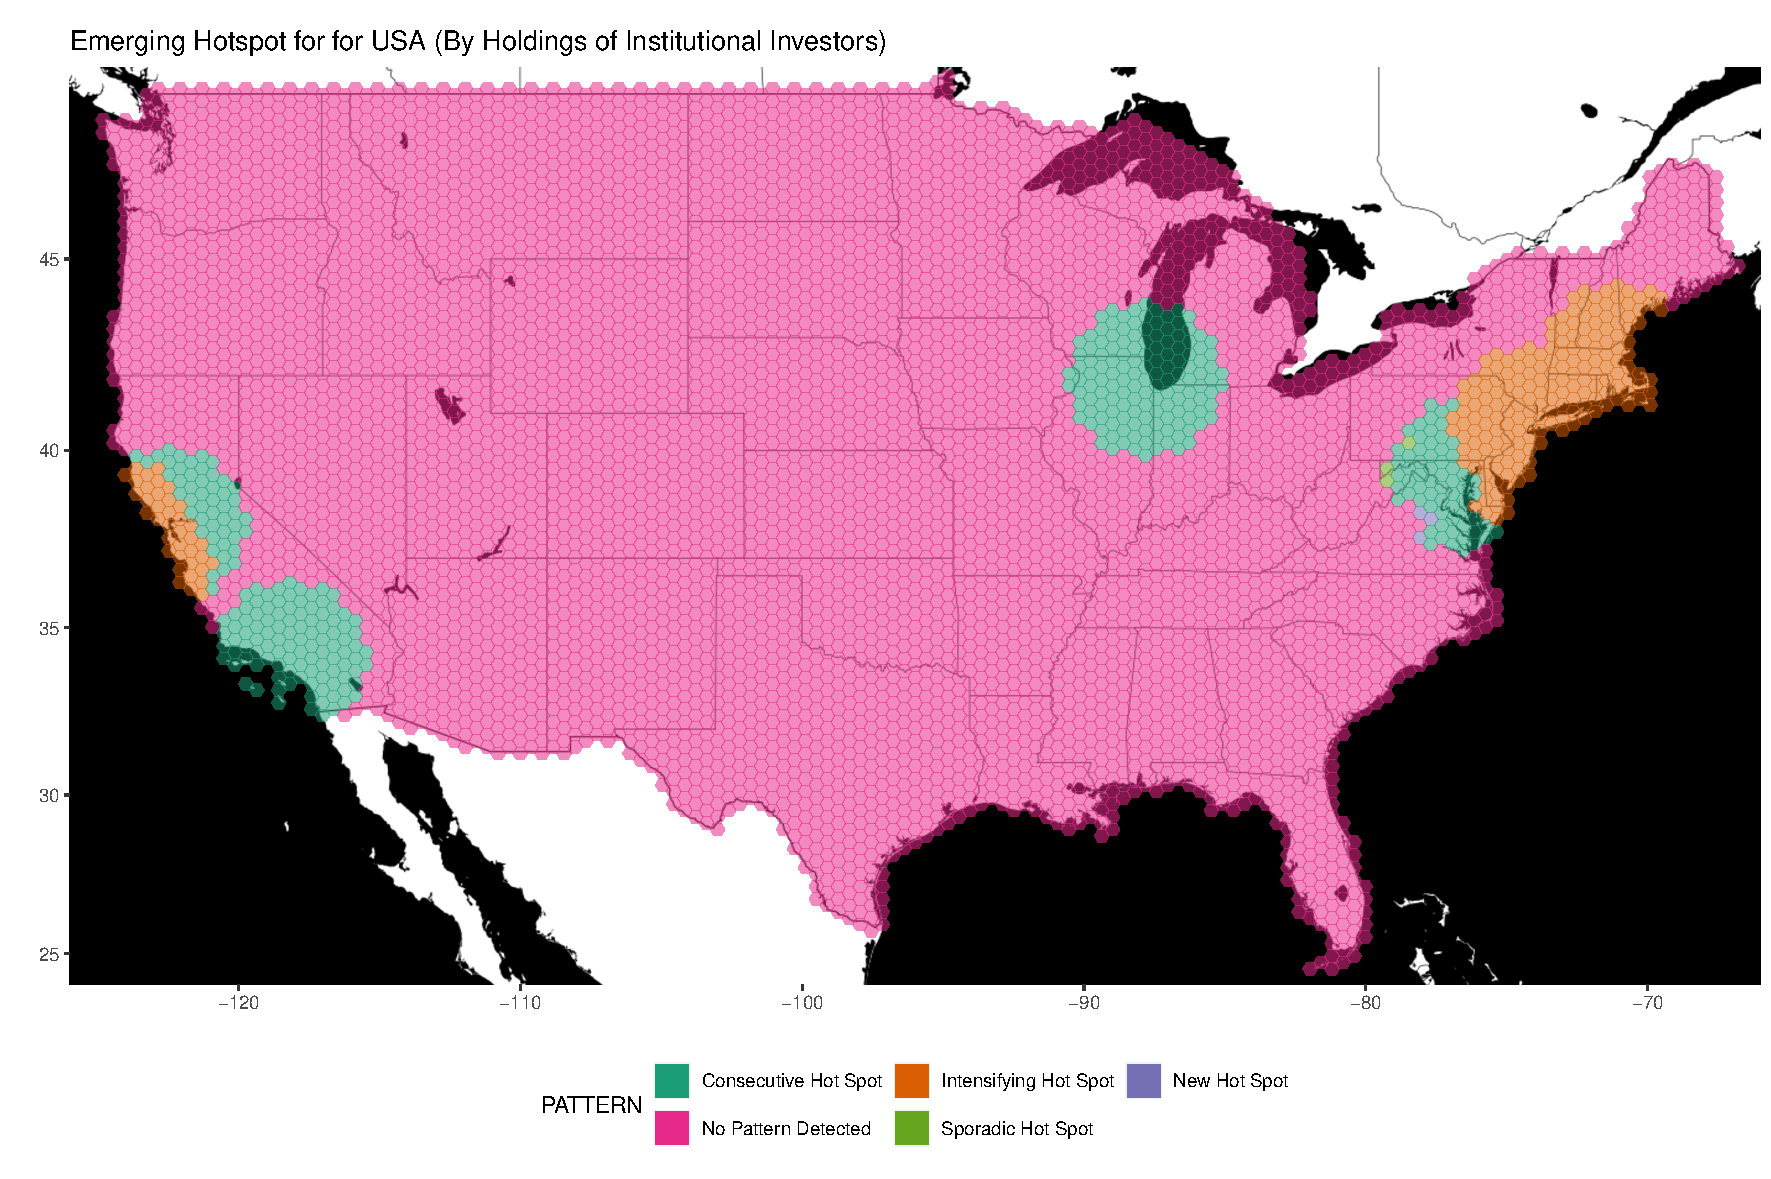
\includegraphics[width=1\linewidth]{Figures/ChapterIV/USA_Money_EH}
	\caption[Local Outlier Analysis of USA-based Institutional Investors 2013-2018]{Local outlier analysis of USA-based institutional investors located in the United States of America for the period of June 2013 to December 2018. }
	\label{fig:usaHSP_Money}
\end{figure}	


As with Figure \ref{fig:usaHSP_Money}, which is based on the holdings database, the local outlier analysis (Figure \ref{fig:usaloamoney}) is much more restrained than the analysis done on the address book database.  Immediately noticeable is the absence of the high-low hexes dotting the capitals of fly-over states, as well as the more restrained presence of low-high clusters in the Bos-NY-Wash.  Lastly, as a lone bright spot in a sea of nothingness, Atlanta is the only place outside of the 5 largest US cities for institutional investment that is a high-high hex.  This is consistent with the trend seen in Chapter \ref{Atlanta} where Atlanta was becoming the financial centre of the US South-East. 

\begin{figure}
	\centering
	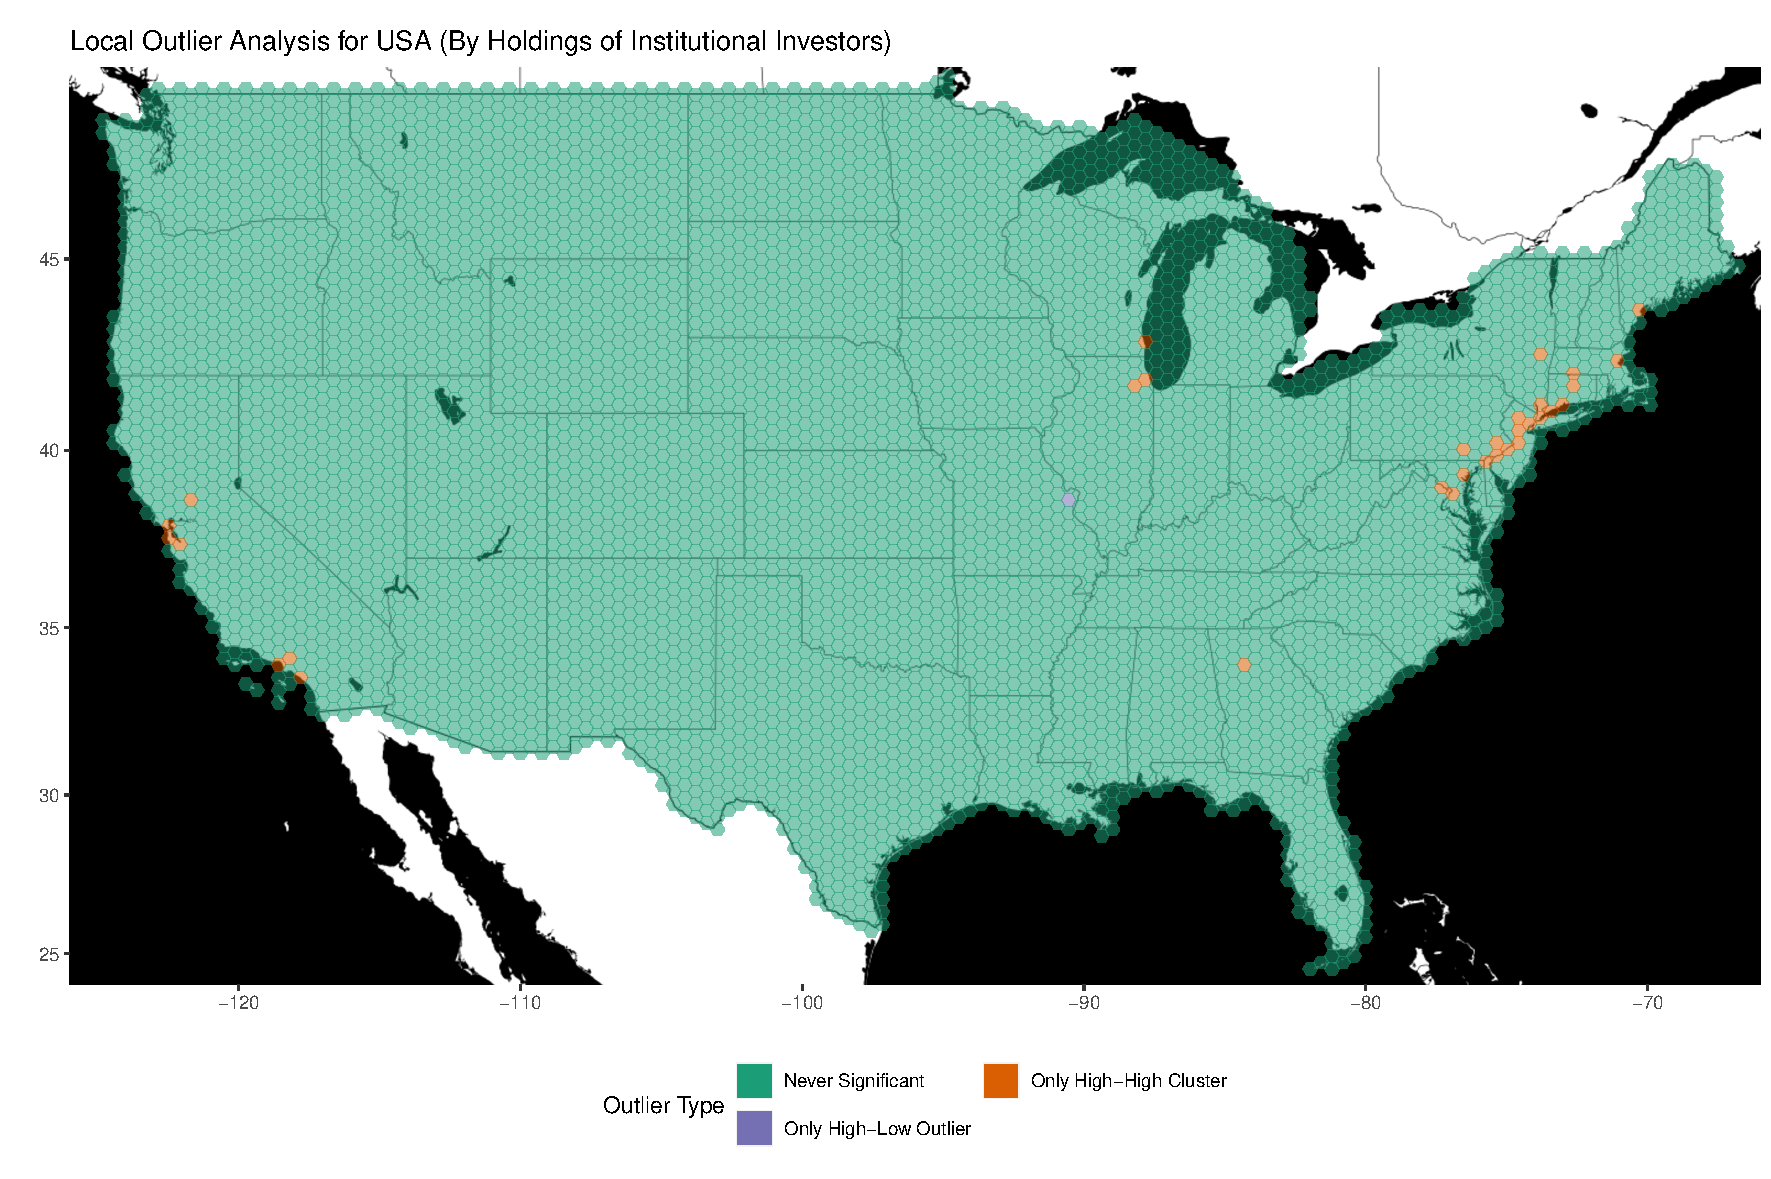
\includegraphics[width=\linewidth]{Figures/ChapterIV/USA_Money_LO}
	\caption[Local Outlier Analysis For Funds Under Management in the United States 2013-2018]{Local outlier analysis for funds under management in the United States for the time period of June 2013 to December 2018.}
	\label{fig:usaloamoney}
\end{figure}


\section{Boston}
\label{subsection:Boston}	
As seen in the various tables and analysis in Chapter \ref{ChapterIIIb}, Boston consistently ranks at the second most important metro area in terms of count of institutional investors and funds under management.  The hex bins for the Boston analysis measure 1 km between horizontal parallels and use a local window radius of 8 km.  In order to make the comparisons between cities meaningful, this scheme of hexagonal grid  and local window size was kept across different metro areas (Chicago, Los Angeles, New York City, and San Francisco).  

\subsection{Count Data}

Figure \ref{fig:bostoncounthotspot} identifies a large cluster covering the areas of Central Boston as well as the southern tip of the Massachusetts Route 128 corridor between the suburban cities of Dedham, Needham and Wellsley.  This cluster essentially contains 3 different types of hot spots.  The first area of central Boston is classified as an intensifying hot spot. This indicates a very high rate of increase in density of institutional investors by hex bin in the area around Boston Commons in downtown Boston.  The second type of hot spot covers the outer periphery of central Boston, as well as the southern arc of Highway 128.  Lastly, the southern part of the community of Dedham contains a sporadic hot spot indicating that this zone sees intermittent changes in institutional investor count over time.  The inclusion of the southern part of the route 128 high tech corridor in the investment cluster isn't surprising considering the long history of partnership between high tech research and development and finance capital \citep{kenney1999technology}.  

\begin{figure}
	\centering
	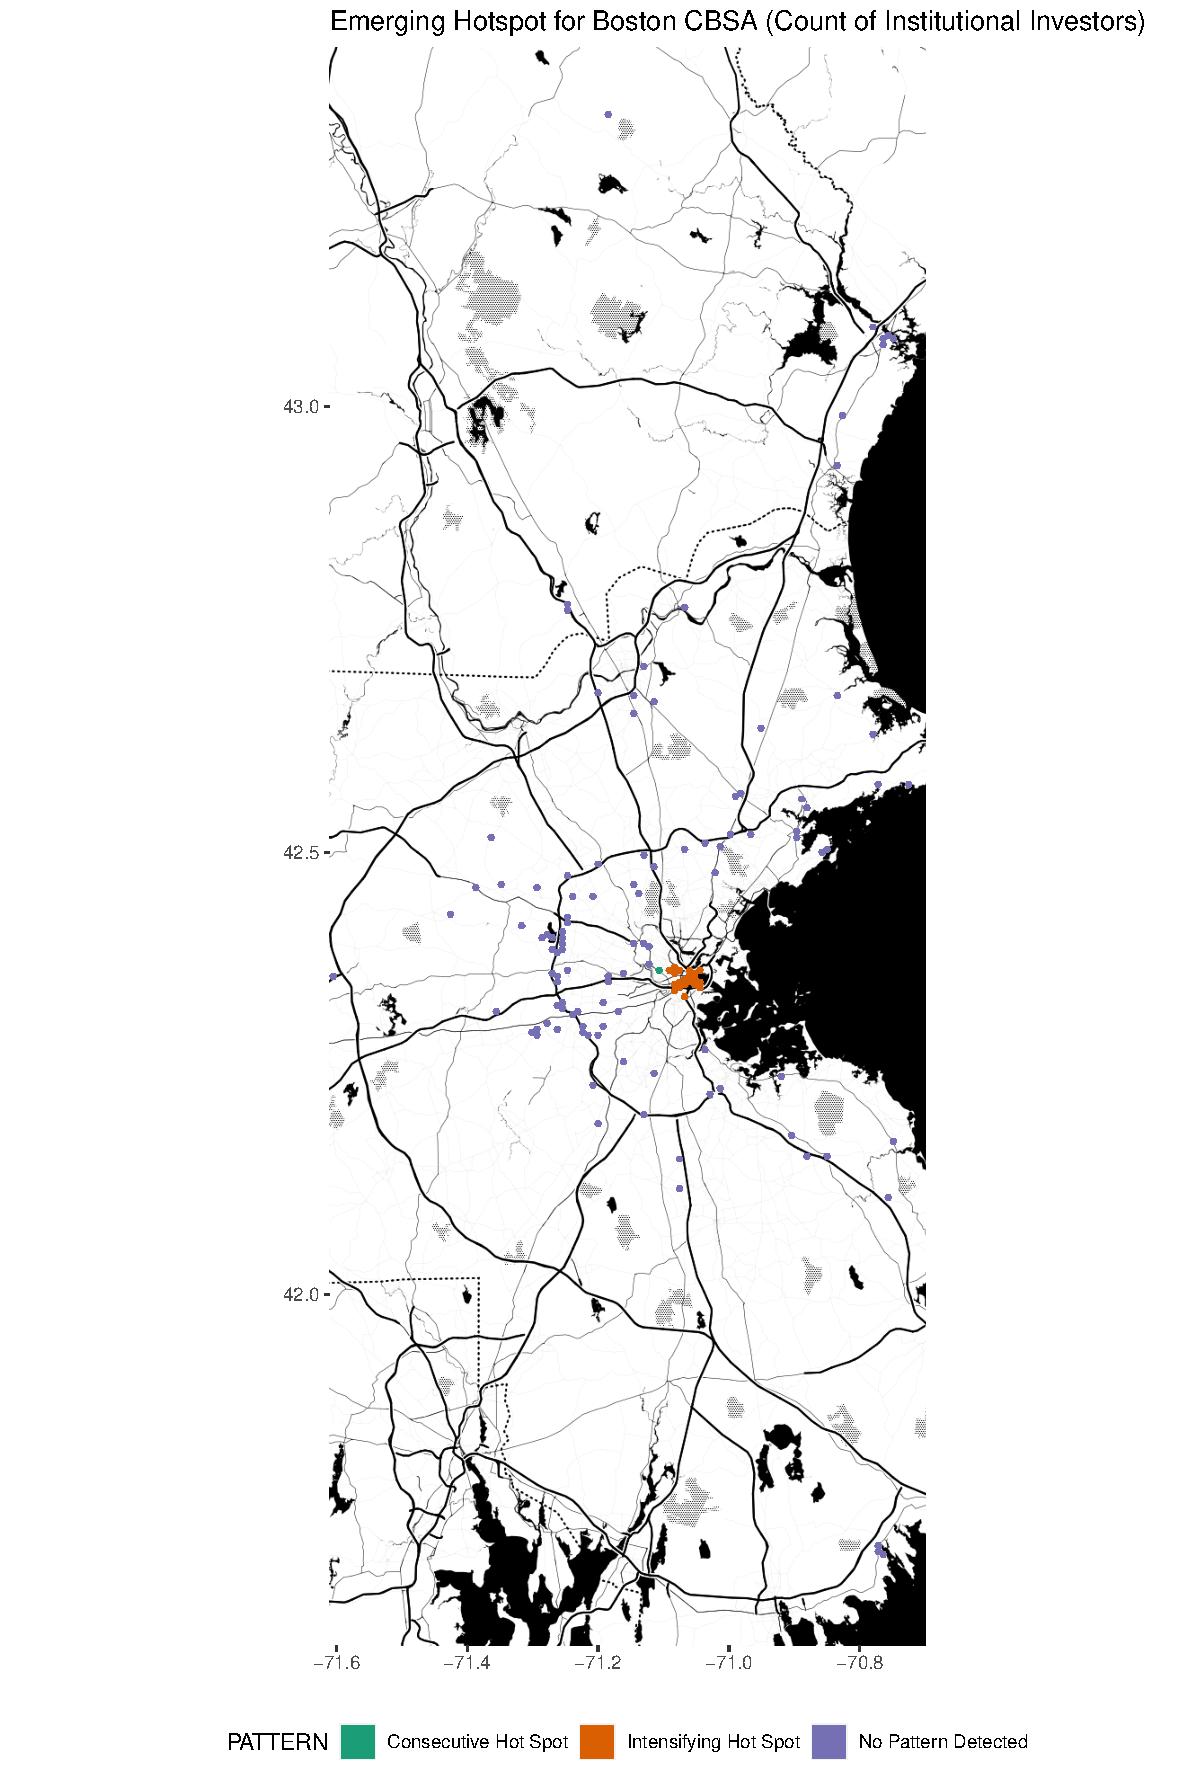
\includegraphics[width=1\linewidth]{Figures/ChapterIV/Bos_Count_EH}
	\caption[Hot Spot Analysis of Number of Firms in Boston CBSA 1999-2018]{Hot spot analysis of number of firms in Boston CBSA for the time period March 1999 to December 2018}
	\label{fig:bostoncounthotspot}
\end{figure}

Figure \ref{fig:bostoncountlocaloutliercount} displays of local outlier analysis confirms the importance of both central Boston as well as the southern arch of the route 128 corridor.   	

\begin{figure}
	\centering
	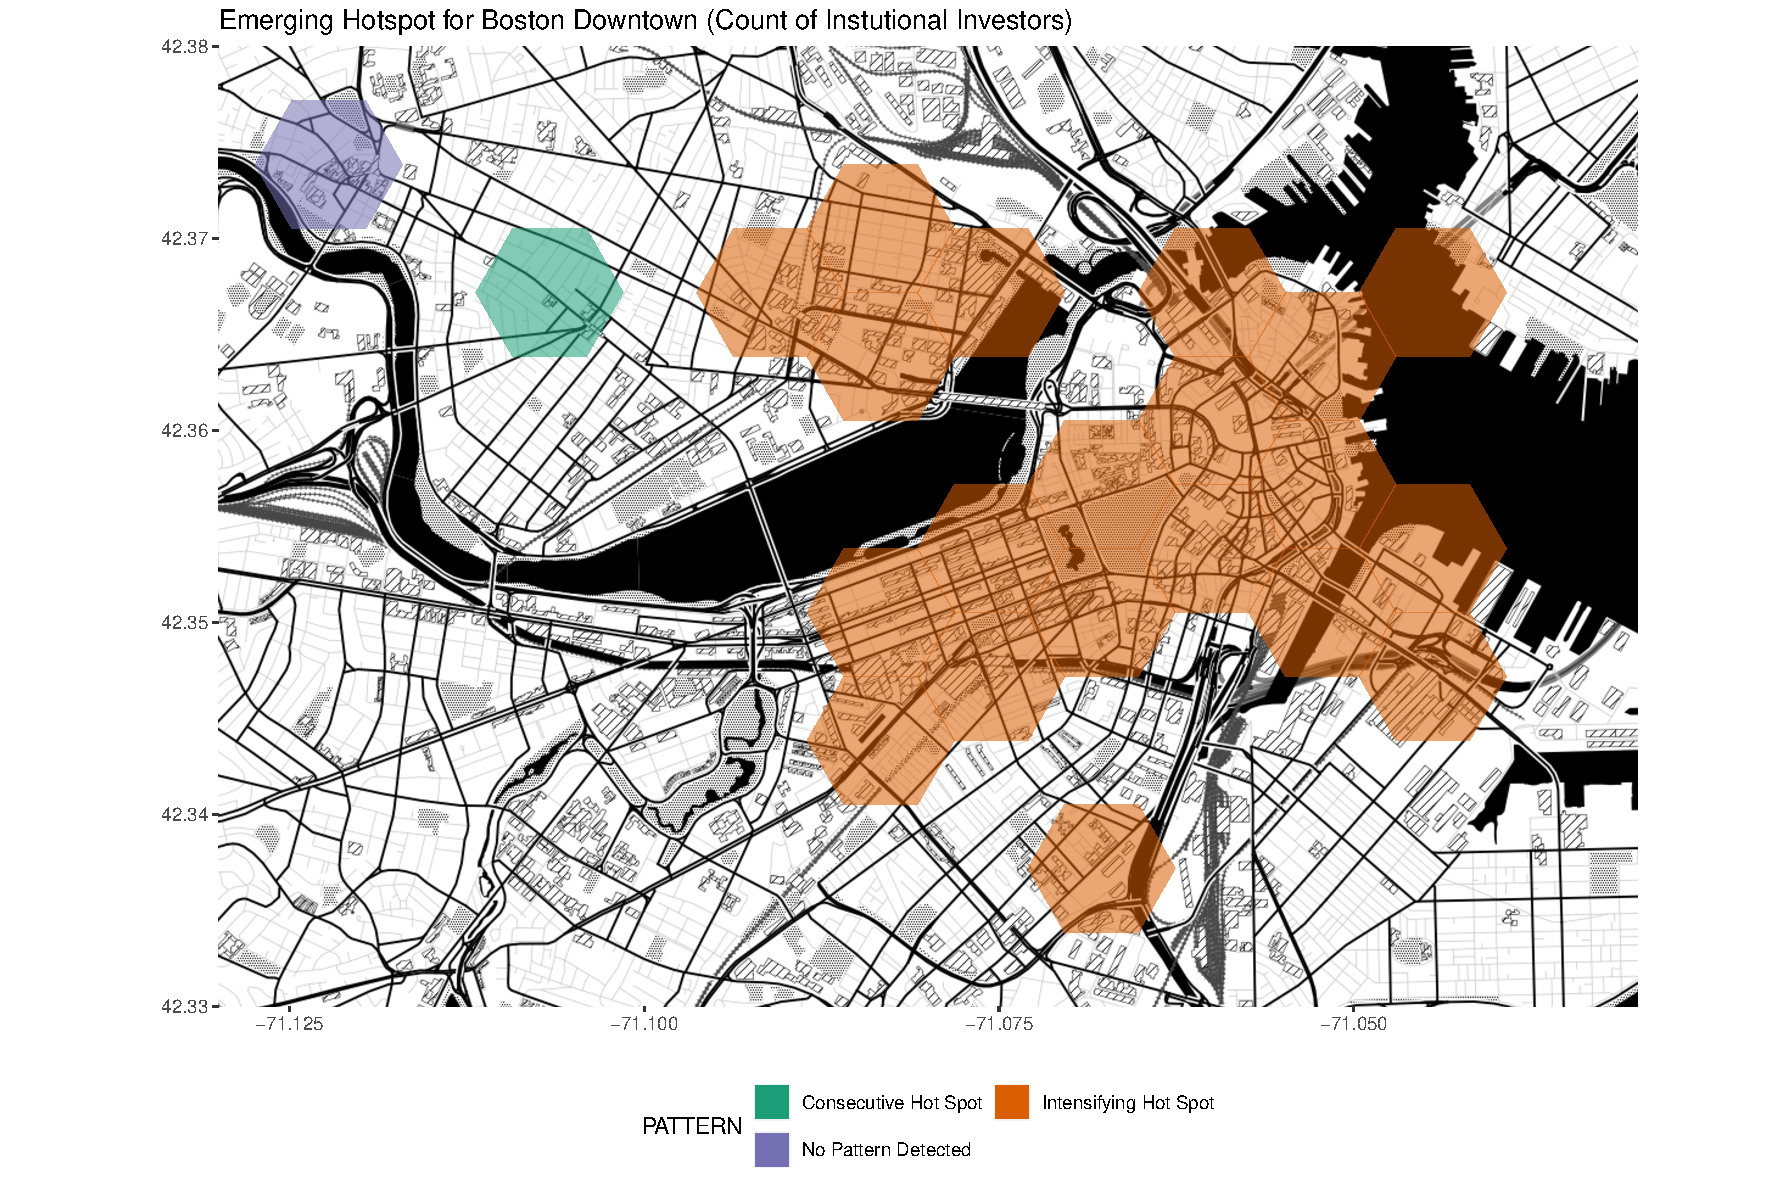
\includegraphics[width=1\linewidth]{Figures/ChapterIV/Bos_Count_EH_Downtown}
	\caption[Hot Spot Analysis of Number of Firms in Downtown Boston 1999-2018]{Hot spot analysis of number of firms in downtown Boston for the time period March 1999 to December 2018}
	\label{fig:bostoncounthotspot_Downtown}
\end{figure}

\begin{figure}
	\centering
	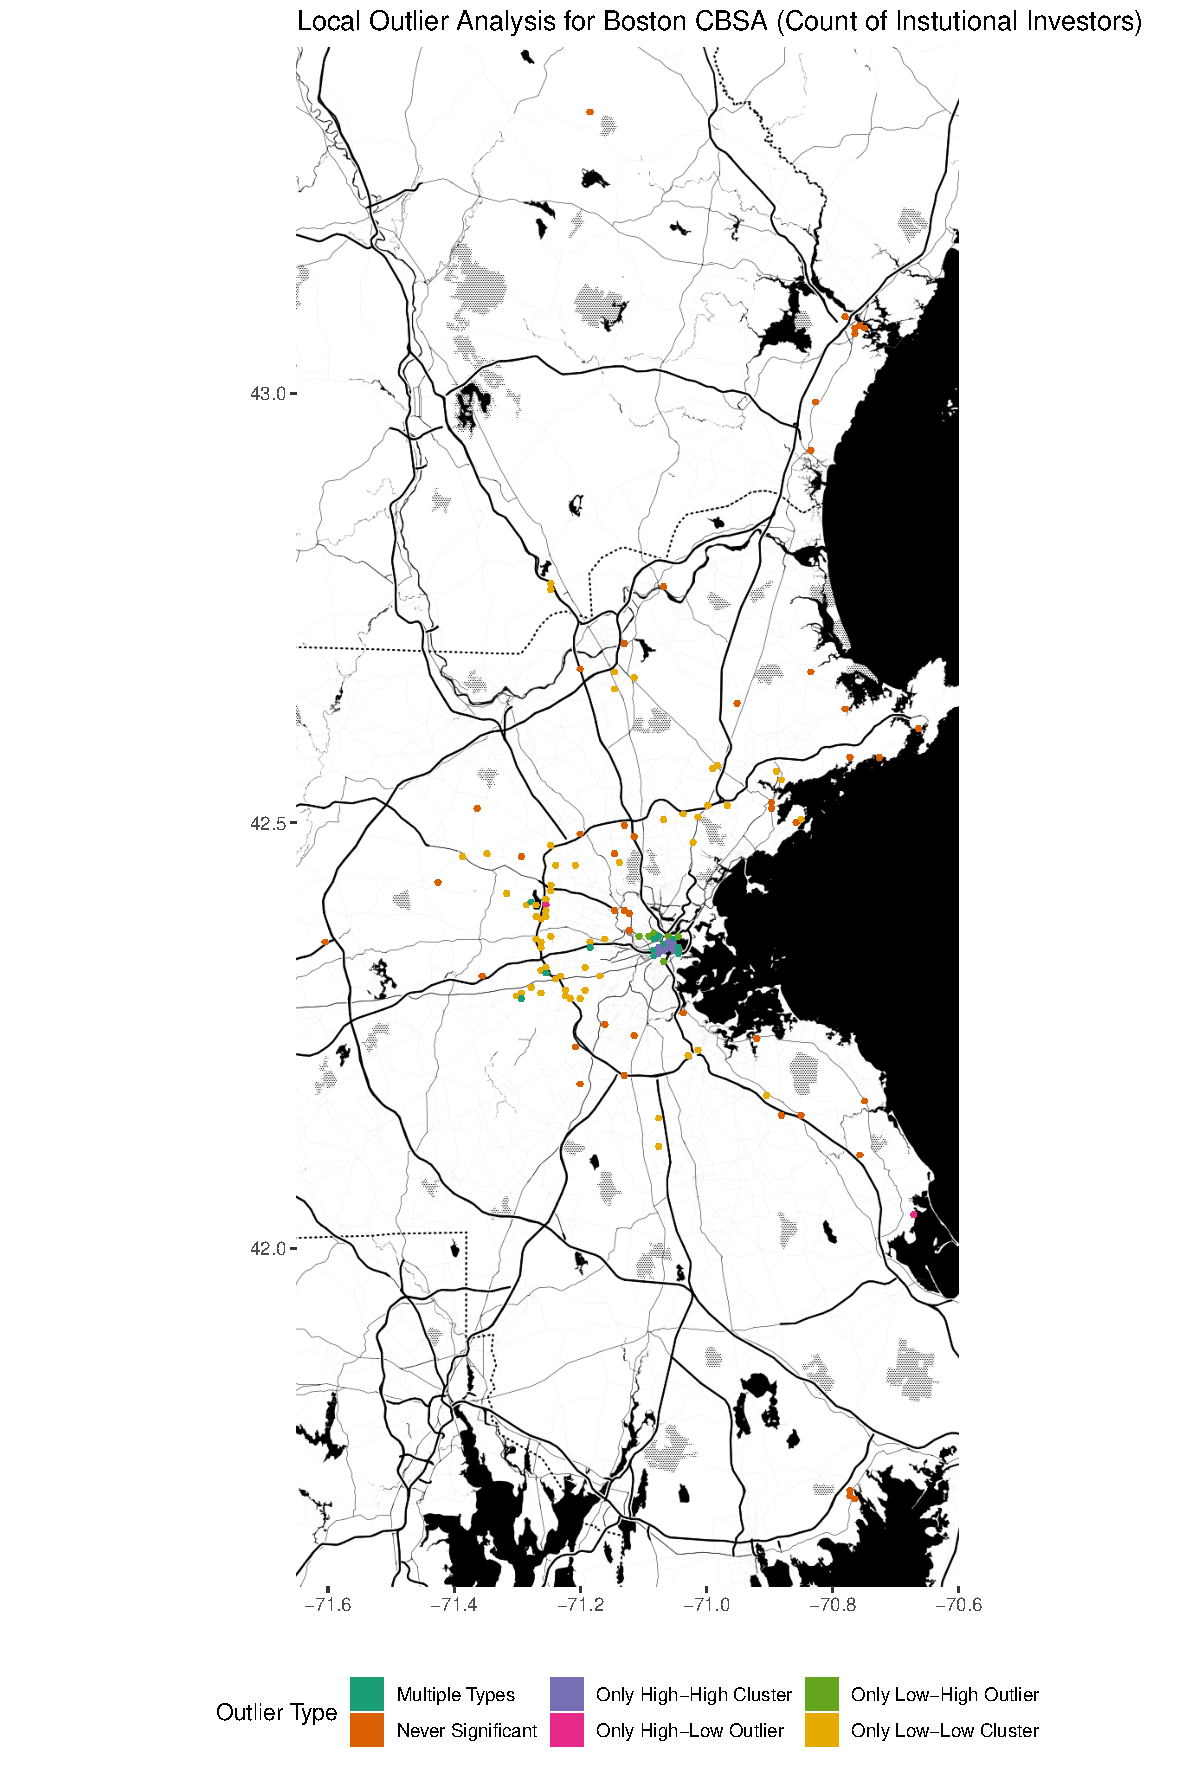
\includegraphics[width=1\linewidth]{Figures/ChapterIV/Bos_Count_LO}
	\caption[Boston CBSA Local Outlier Analysis - Count of Institutional Investors 1999-2018]{Boston CBSA local outlier analysis - count of institutional investors}
	\label{fig:bostoncountlocaloutliercount}
\end{figure}

\begin{figure}
	\centering
	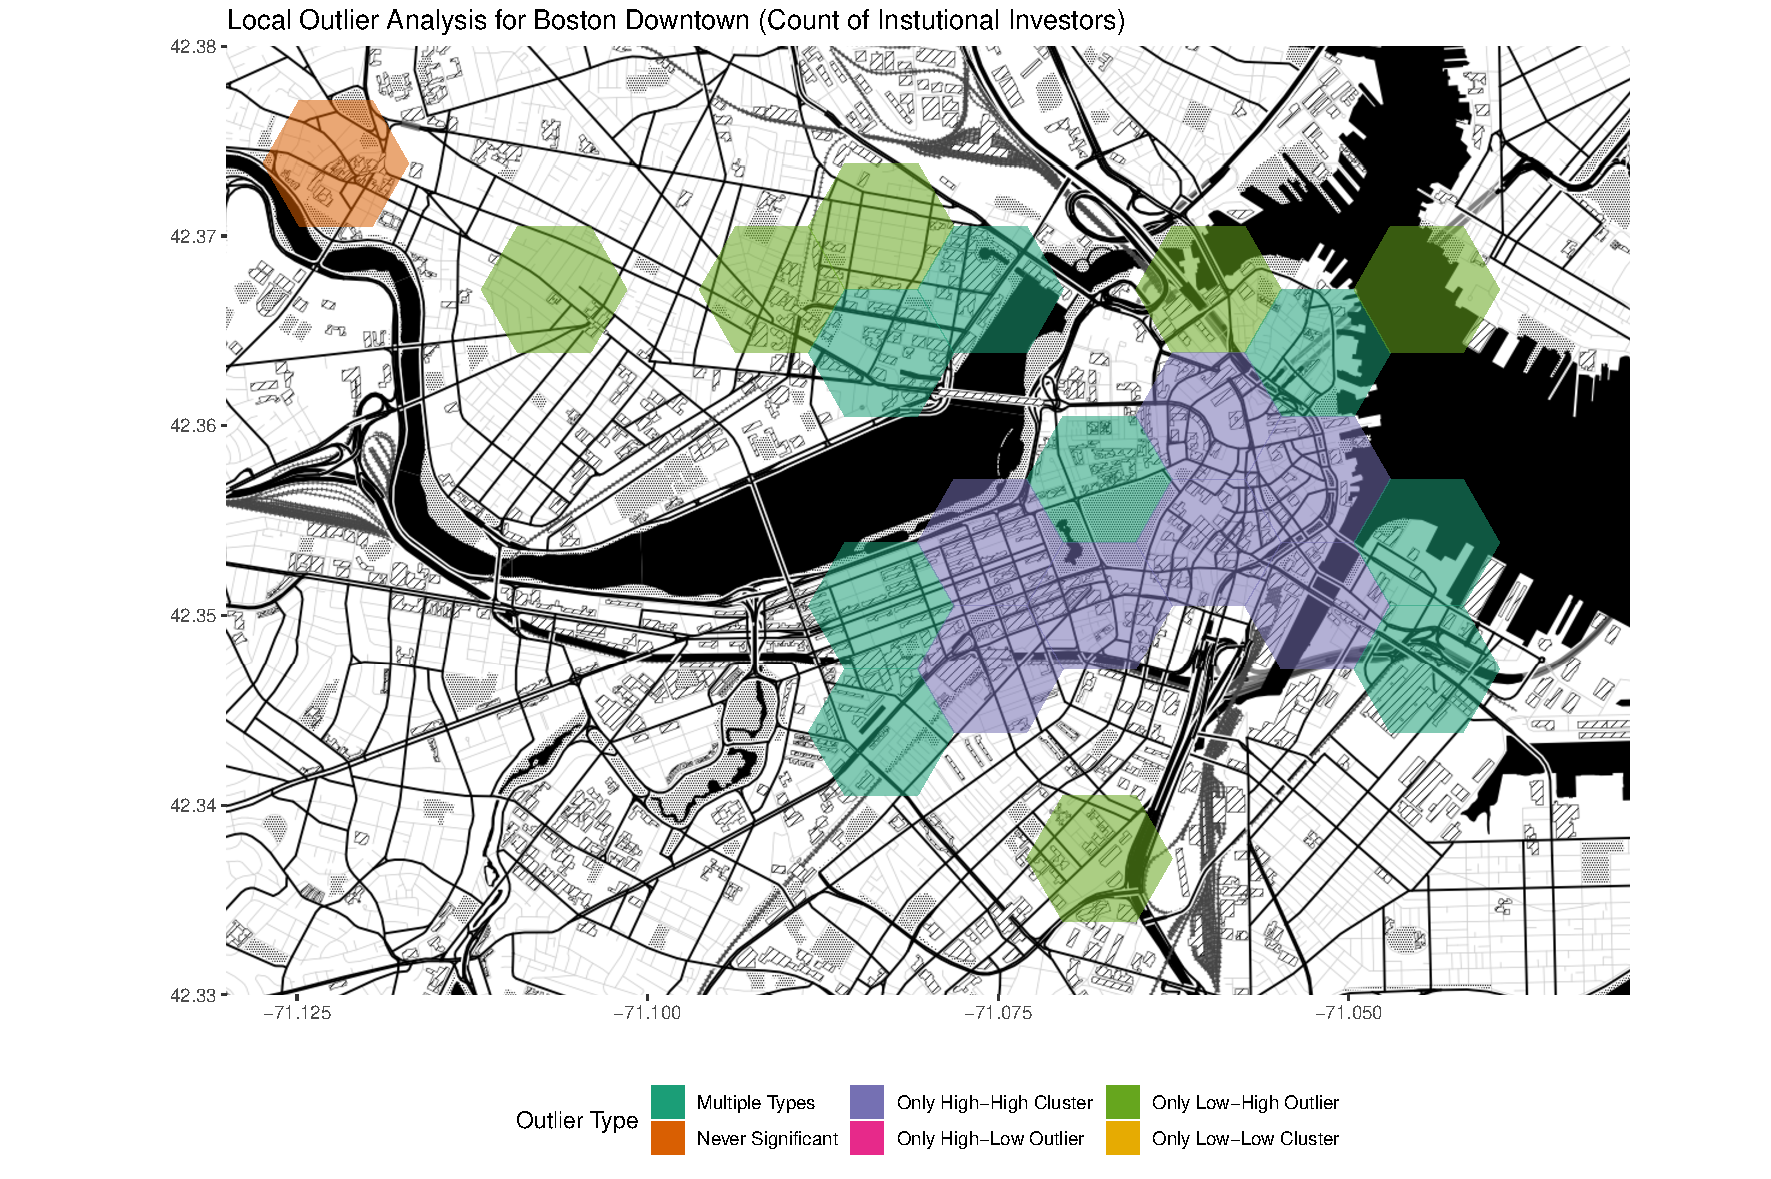
\includegraphics[width=1\linewidth]{Figures/ChapterIV/Bos_Count_LO_Downtown}
	\caption[Downtown Boston Local Outlier Analysis - Count of Institutional Investors 1999-2018]{Downtown Boston local outlier analysis - count of institutional investors}
	\label{fig:bostoncountlocaloutliercount_Downtown}
\end{figure}


\subsection{Funds Under Management}

Unlike Figure \ref{fig:bostoncounthotspot}'s larger cluster, the emerging hot spot analysis in Figure \ref{fig:bostonmoneyhotspot} using funds under management as a criteria is more exclusionary since it only contains central Boston and ignores the Massachusetts Route 128 corridor.  A partial explanation for this is the high collection of bank and insurance based institutional investors located in Boston's financial district that abuts Boston Common .    	

\begin{figure}
	\centering
	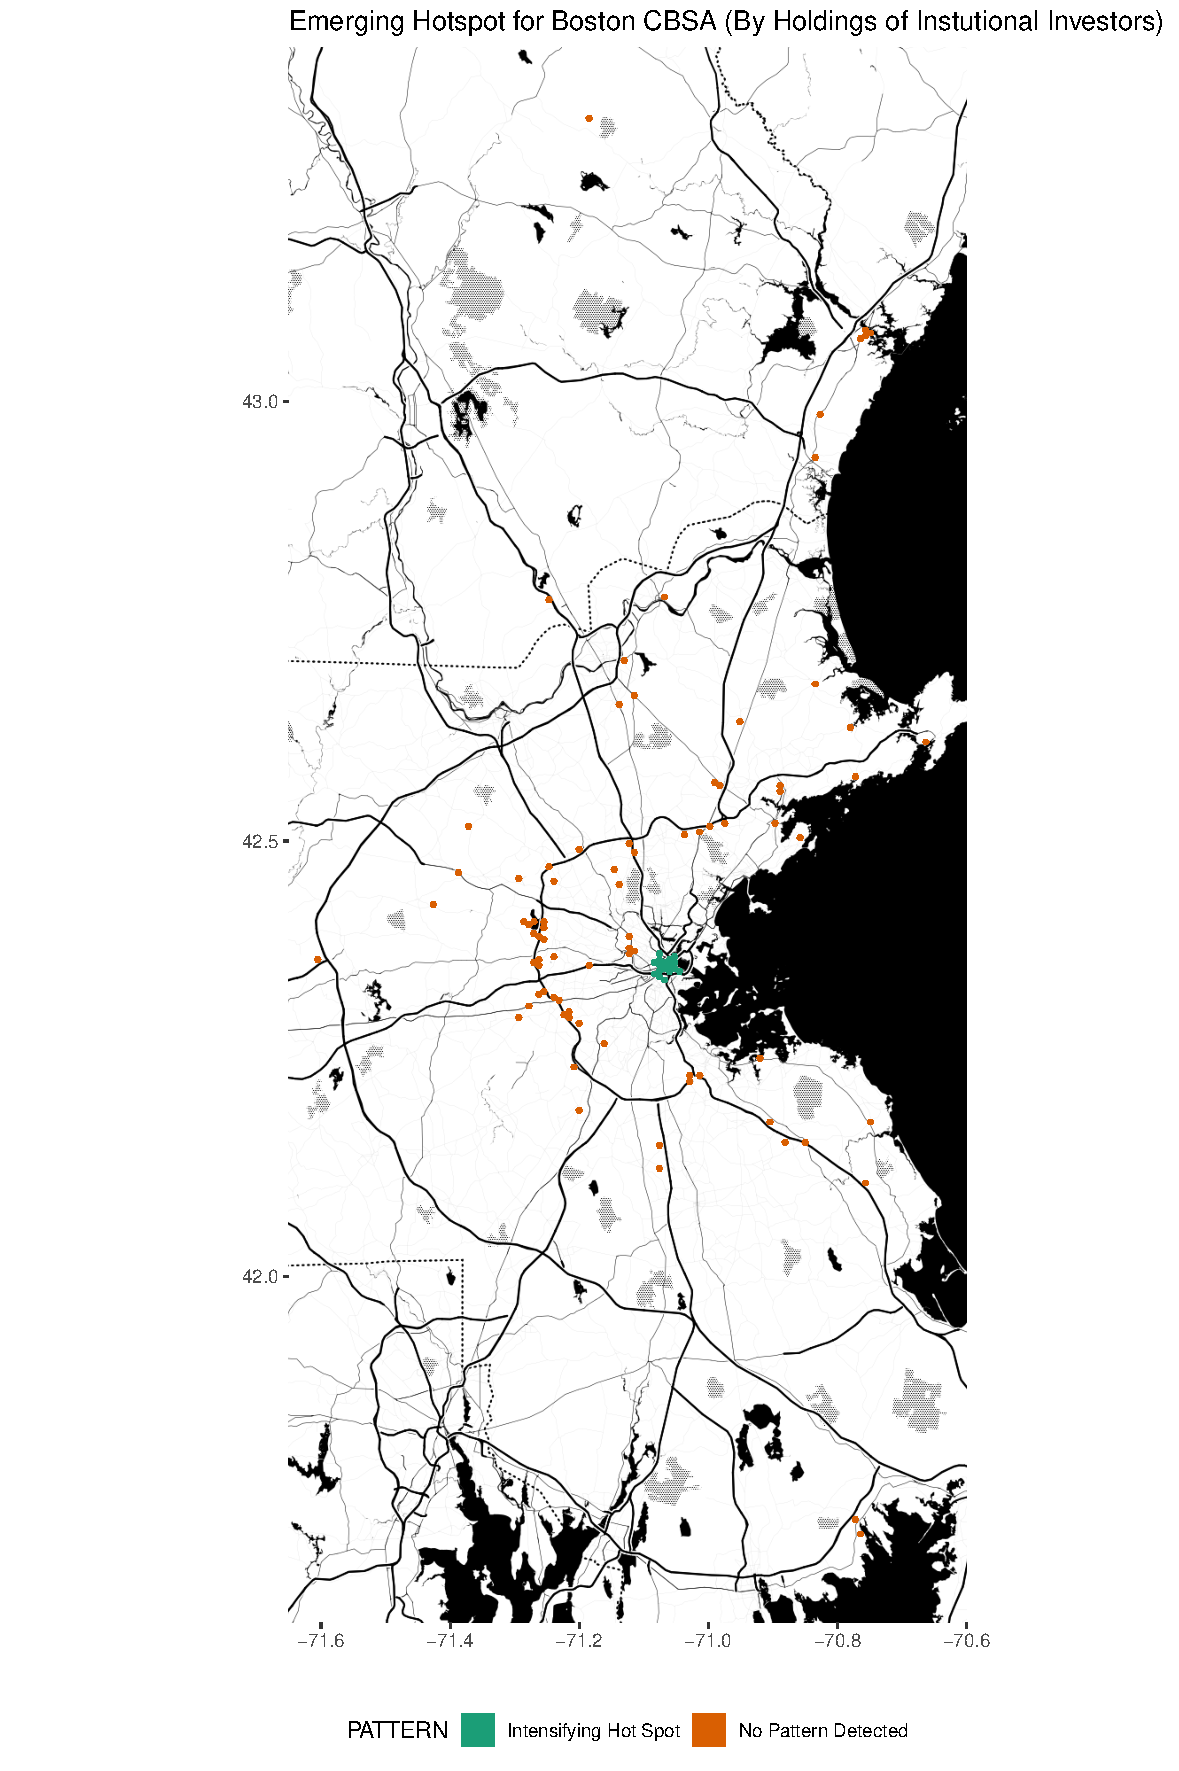
\includegraphics[width=1\linewidth]{Figures/ChapterIV/Bos_Money_EH}
	\caption[Emerging Hot Spot Analysis of Funds Under Management for Boston CBSA 2013-2018]{Emerging hot spot analysis of funds under management for Boston CBSA for period June 2013 to December 2018}
	\label{fig:bostonmoneyhotspot}
\end{figure}

\begin{figure}
	\centering
	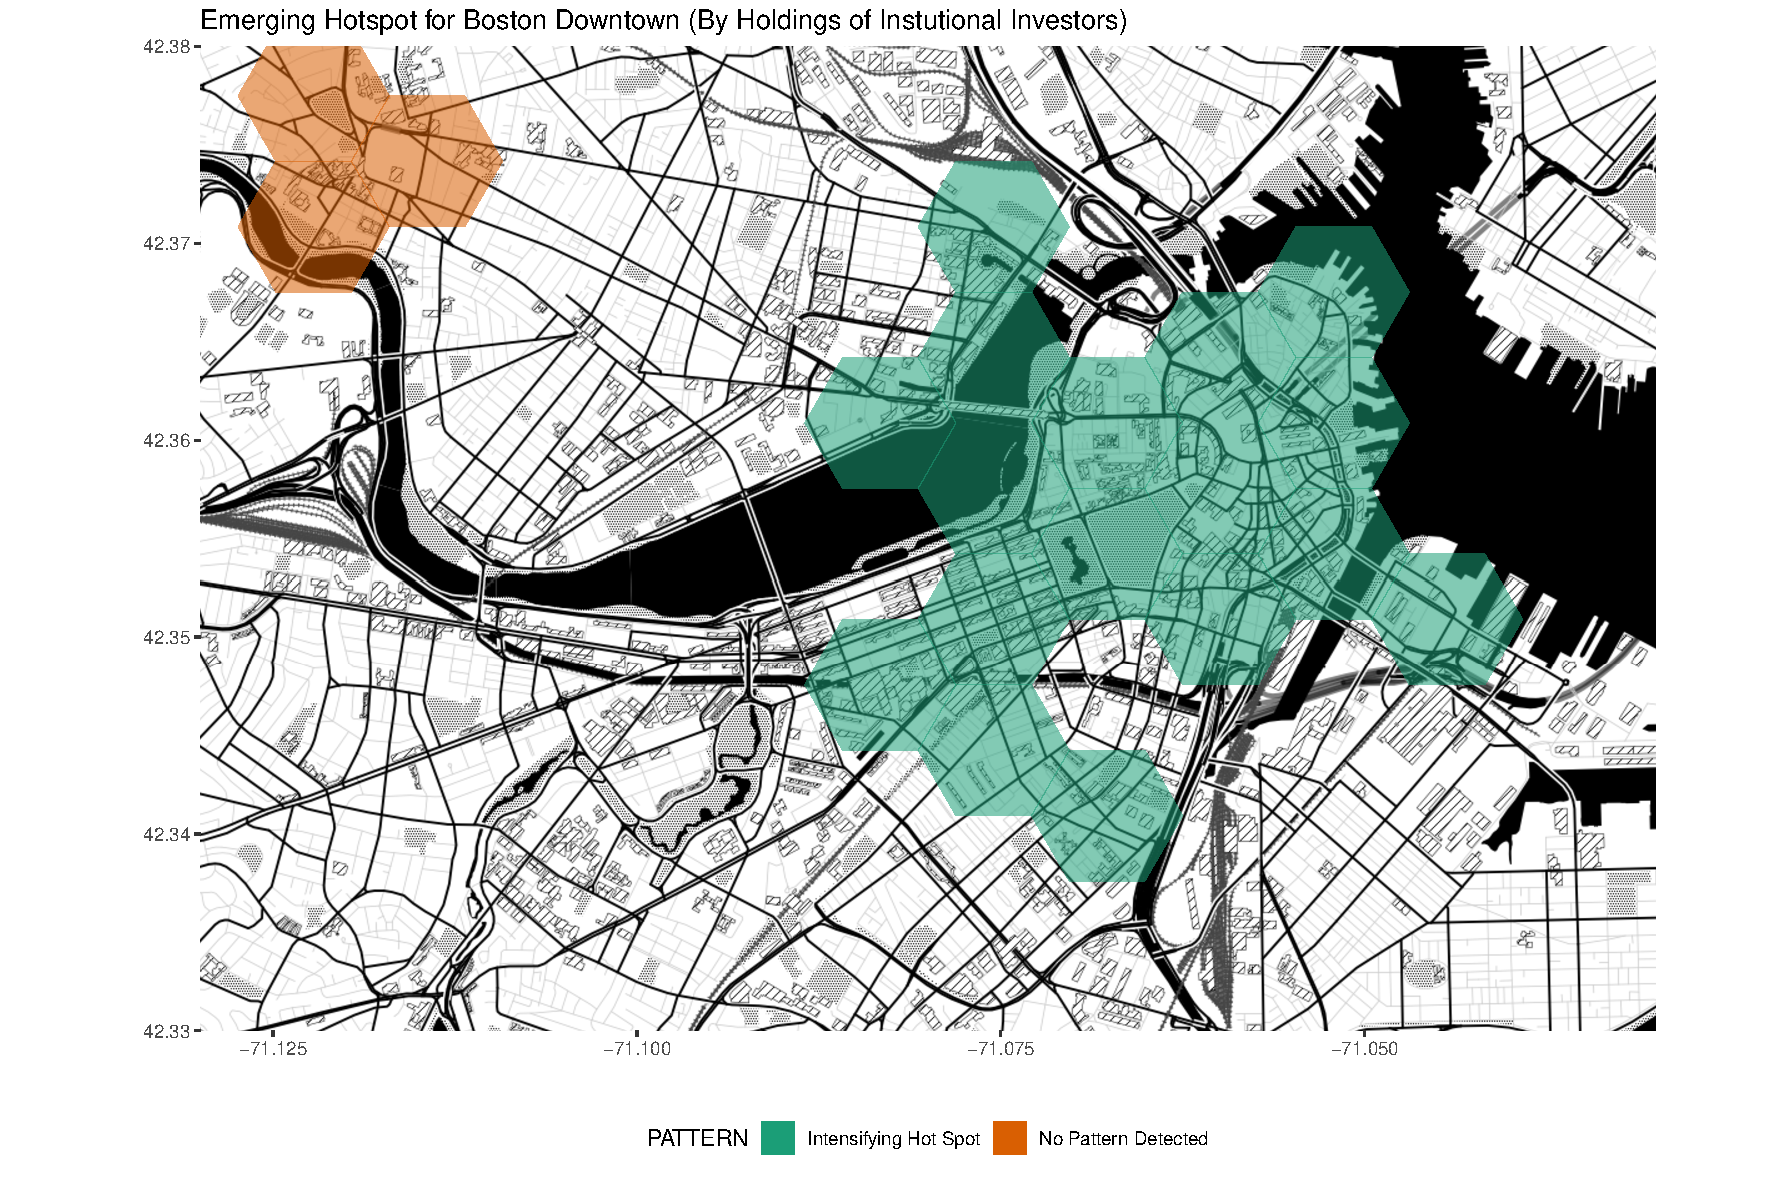
\includegraphics[width=1\linewidth]{Figures/ChapterIV/Bos_Money_EH_Downtown}
	\caption[Emerging Hot Spot Analysis of Funds Under Management for Downtown Boston 2013-2018]{Emerging hot spot analysis of funds under management for downtown Boston for period June 2013 to December 2018}
	\label{fig:bostonmoneyhotspot_Downtown}
\end{figure}


Following in a similar theme to Figure \ref{fig:bostonmoneyhotspot}, the local outlier analysis only finds high-high clusters in central Boston. Interestingly, the model accurately picks out Boston Common as a non-cluster.  A look at the region shows that many institutional investors surround this 25 hectare urban park, and this creates a discontinuity.  

\begin{figure}
	\centering
	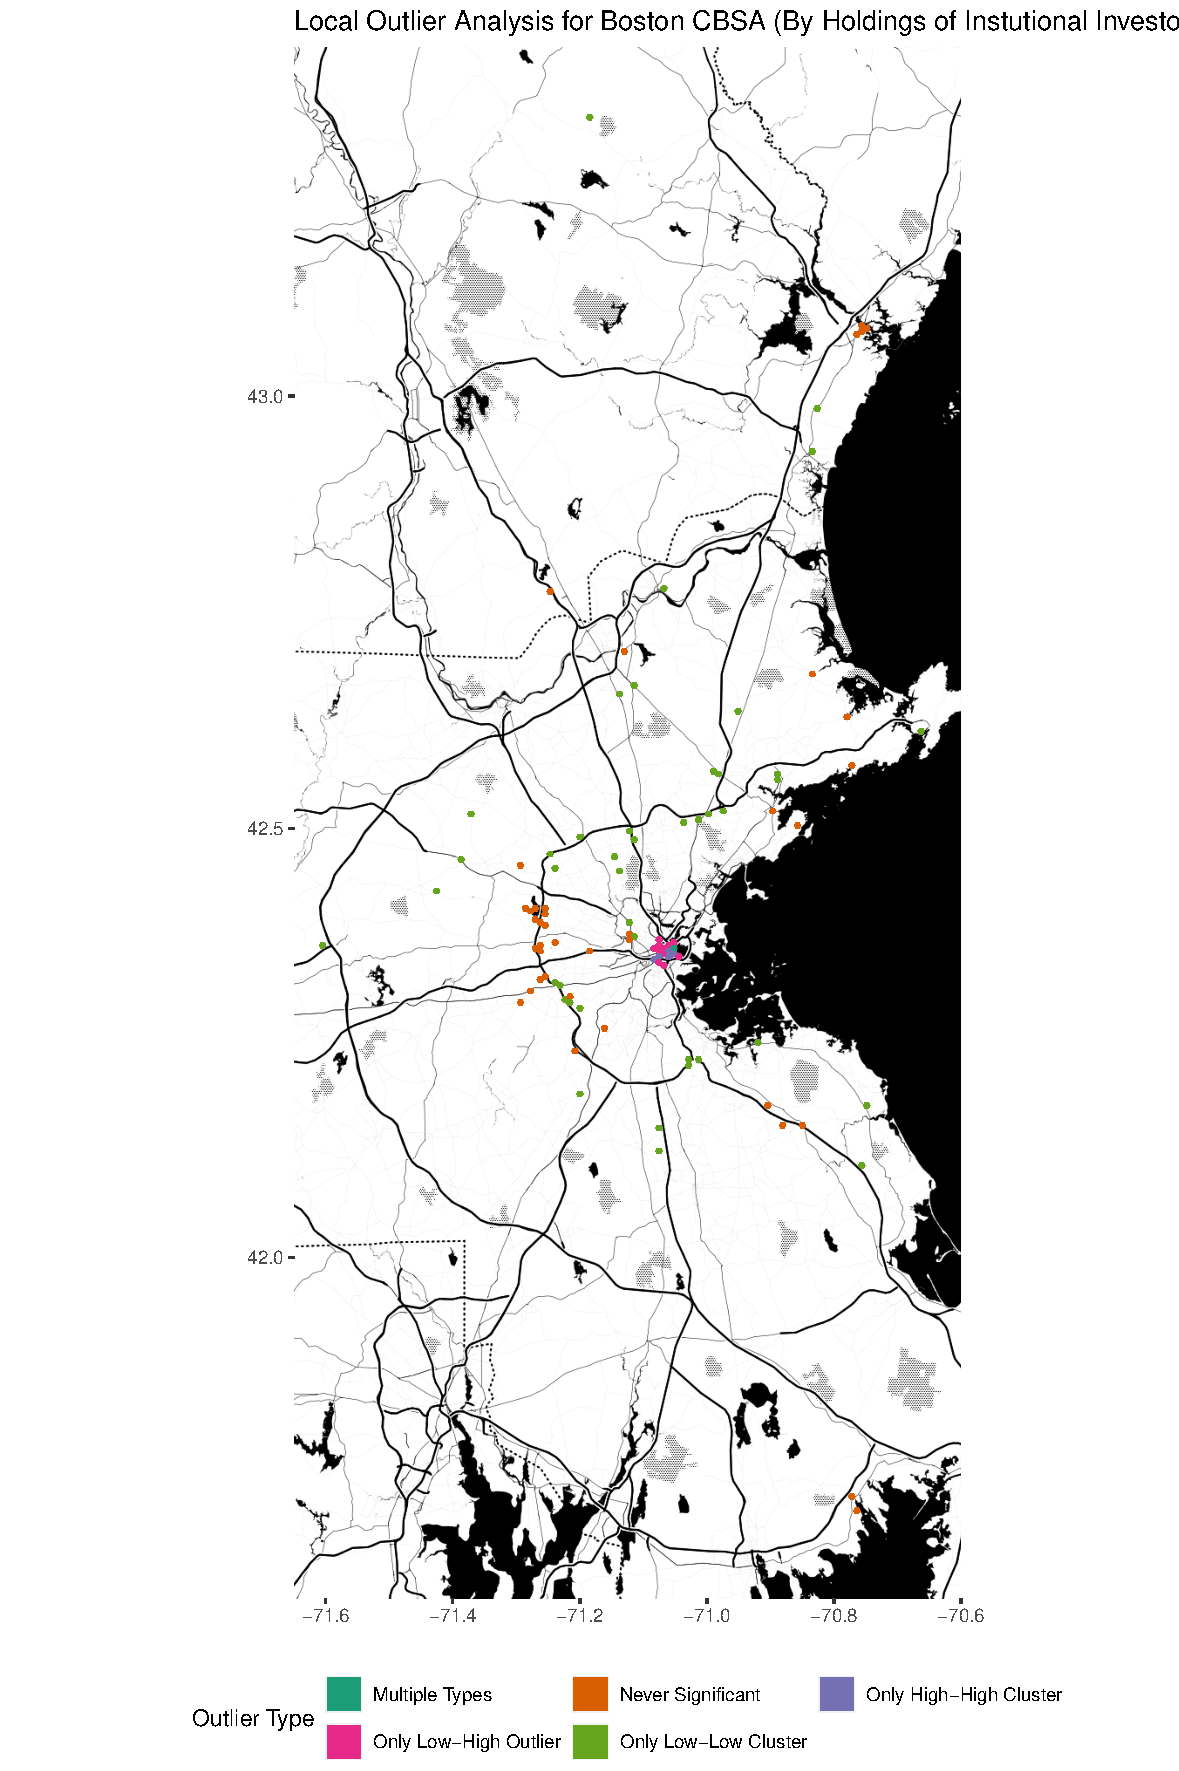
\includegraphics[width=1\linewidth]{Figures/ChapterIV/Bos_Money_LO}
	\caption[Boston CBSA Local Outlier Analysis - Funds Under Management 2013-2018]{Boston CBSA local outlier analysis - funds under management}
	\label{fig:bostonlocaloutlier}
\end{figure}


\begin{figure}
	\centering
	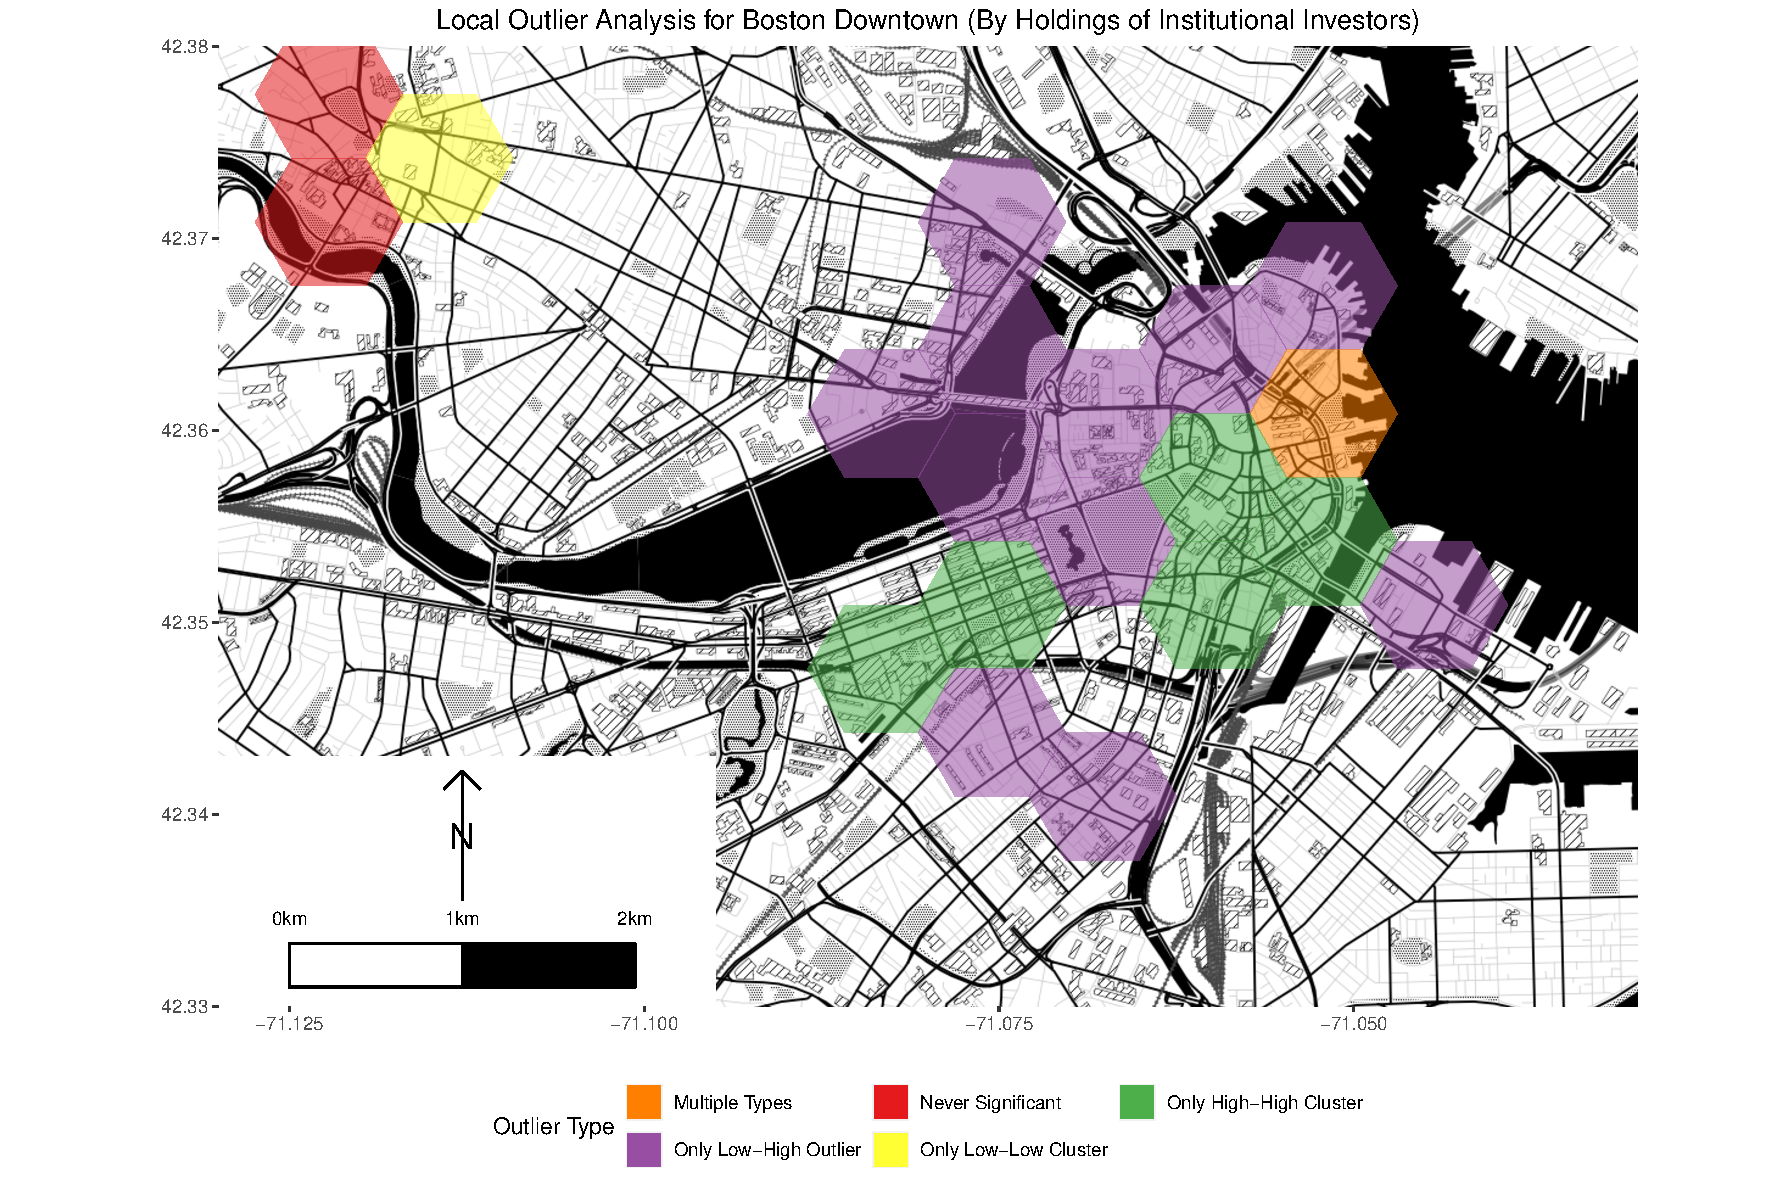
\includegraphics[width=1\linewidth]{Figures/ChapterIV/Bos_Money_LO_Downtown}
	\caption[Boston Downtown Local Outlier Analysis - Funds Under Management 2013-2018]{Boston Downtown local outlier analysis - funds under management}
	\label{fig:bostonlocaloutlier_Downtown}
\end{figure}



\section{Chicago}

\subsection{Count Data}
As displayed in Figure \ref{fig:Chicagocounthotspot}, Chicago contains one intensifying hot spot in the Chicago Loop neighbourhood, including satellite hot spots in the Napierville-Aurora suburb to the West, as well as Evanston and Highland Park to the North.  
\begin{figure}
	\centering
	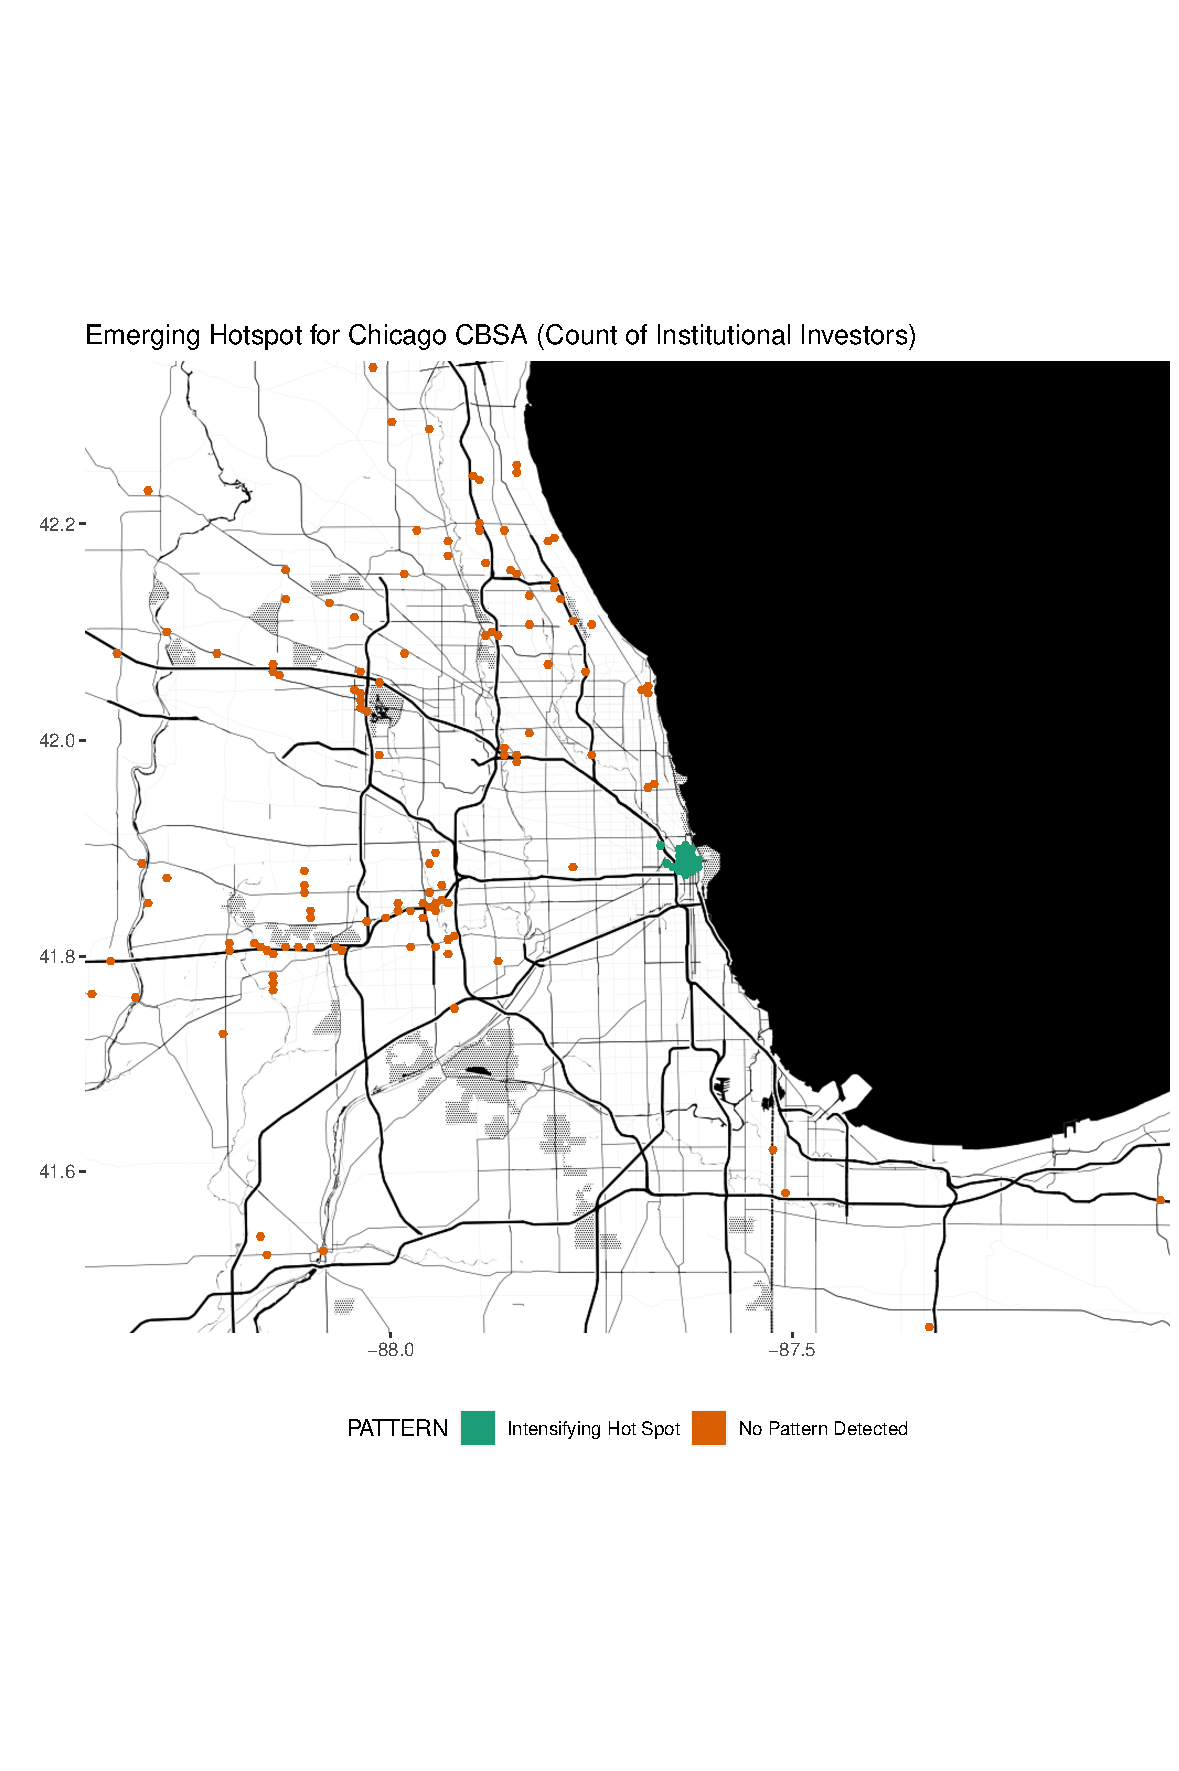
\includegraphics[width=1\linewidth]{Figures/ChapterIV/Chi_Count_EH}
	\caption[Hot Spot Analysis of Number of Firms in Chicago CBSA 1999-2018]{Hot spot analysis of number of firms in Chicago for the time period March 1999 to December 2018}
	\label{fig:Chicagocounthotspot}
\end{figure}

\begin{figure}
	\centering
	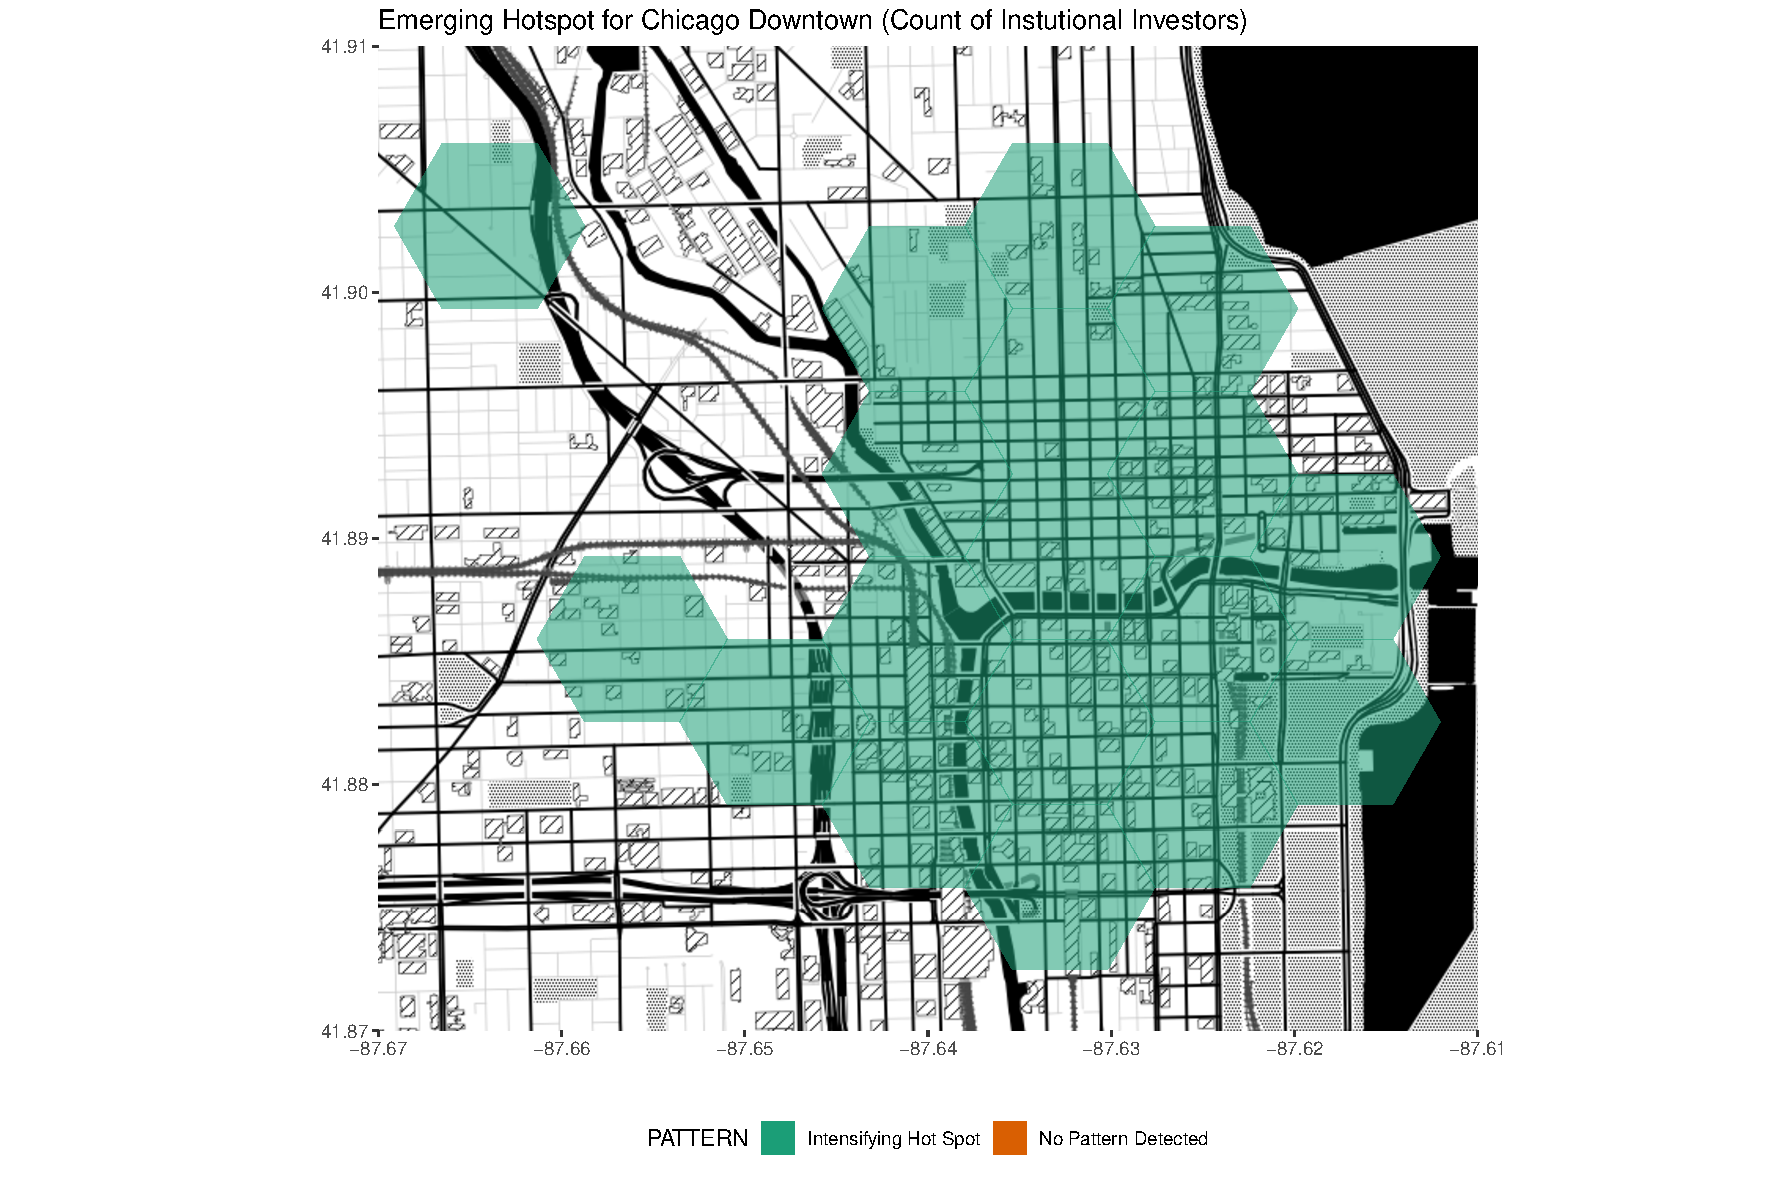
\includegraphics[width=1\linewidth]{Figures/ChapterIV/Chi_Count_EH_Downtown}
	\caption[Hot Spot Analysis of Number of Firms in Downtown Chicago 1999-2018]{Hot spot analysis of number of firms in Chicago for the time period March 1999 to December 2018}
	\label{fig:Chicagocounthotspot_Downtown}
\end{figure}


Using local outlier analysis, only the Loop district contains high-high hexagons. This is consistent with institutional investors perfering CBDs.  Futhermore, there is a conspicuous absence of investors on the South Side of Chicago, however this is not a region of Chicago known for having much financial capital.  
\begin{figure}
	\centering
	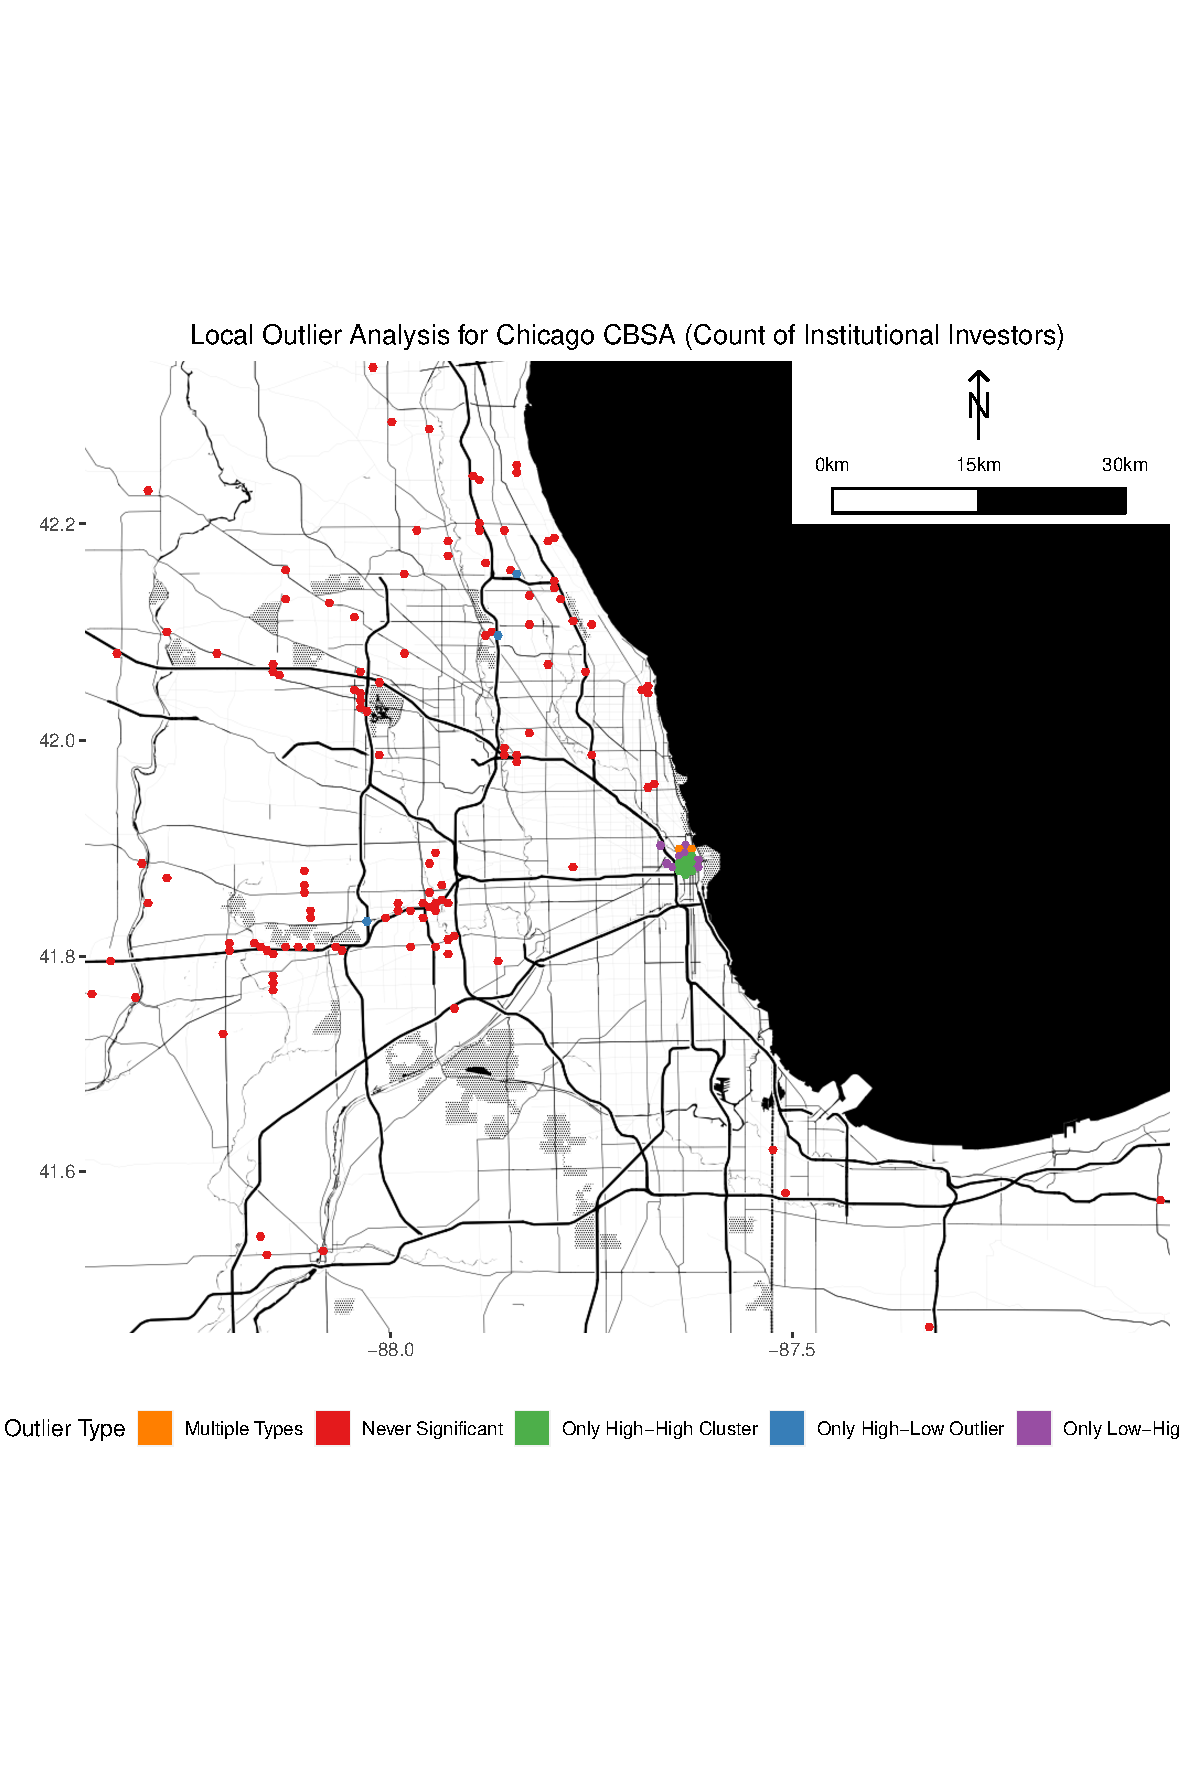
\includegraphics[width=1\linewidth]{Figures/ChapterIV/Chi_Count_LO}
	\caption[Chicago CBSA Local Outlier Analysis - Count of Institutional Investors 1999-2018]{Chicago local outlier analysis - count of institutional investors}
	\label{fig:Chicagocountlocaloutliercount}
\end{figure}	

\begin{figure}
	\centering
	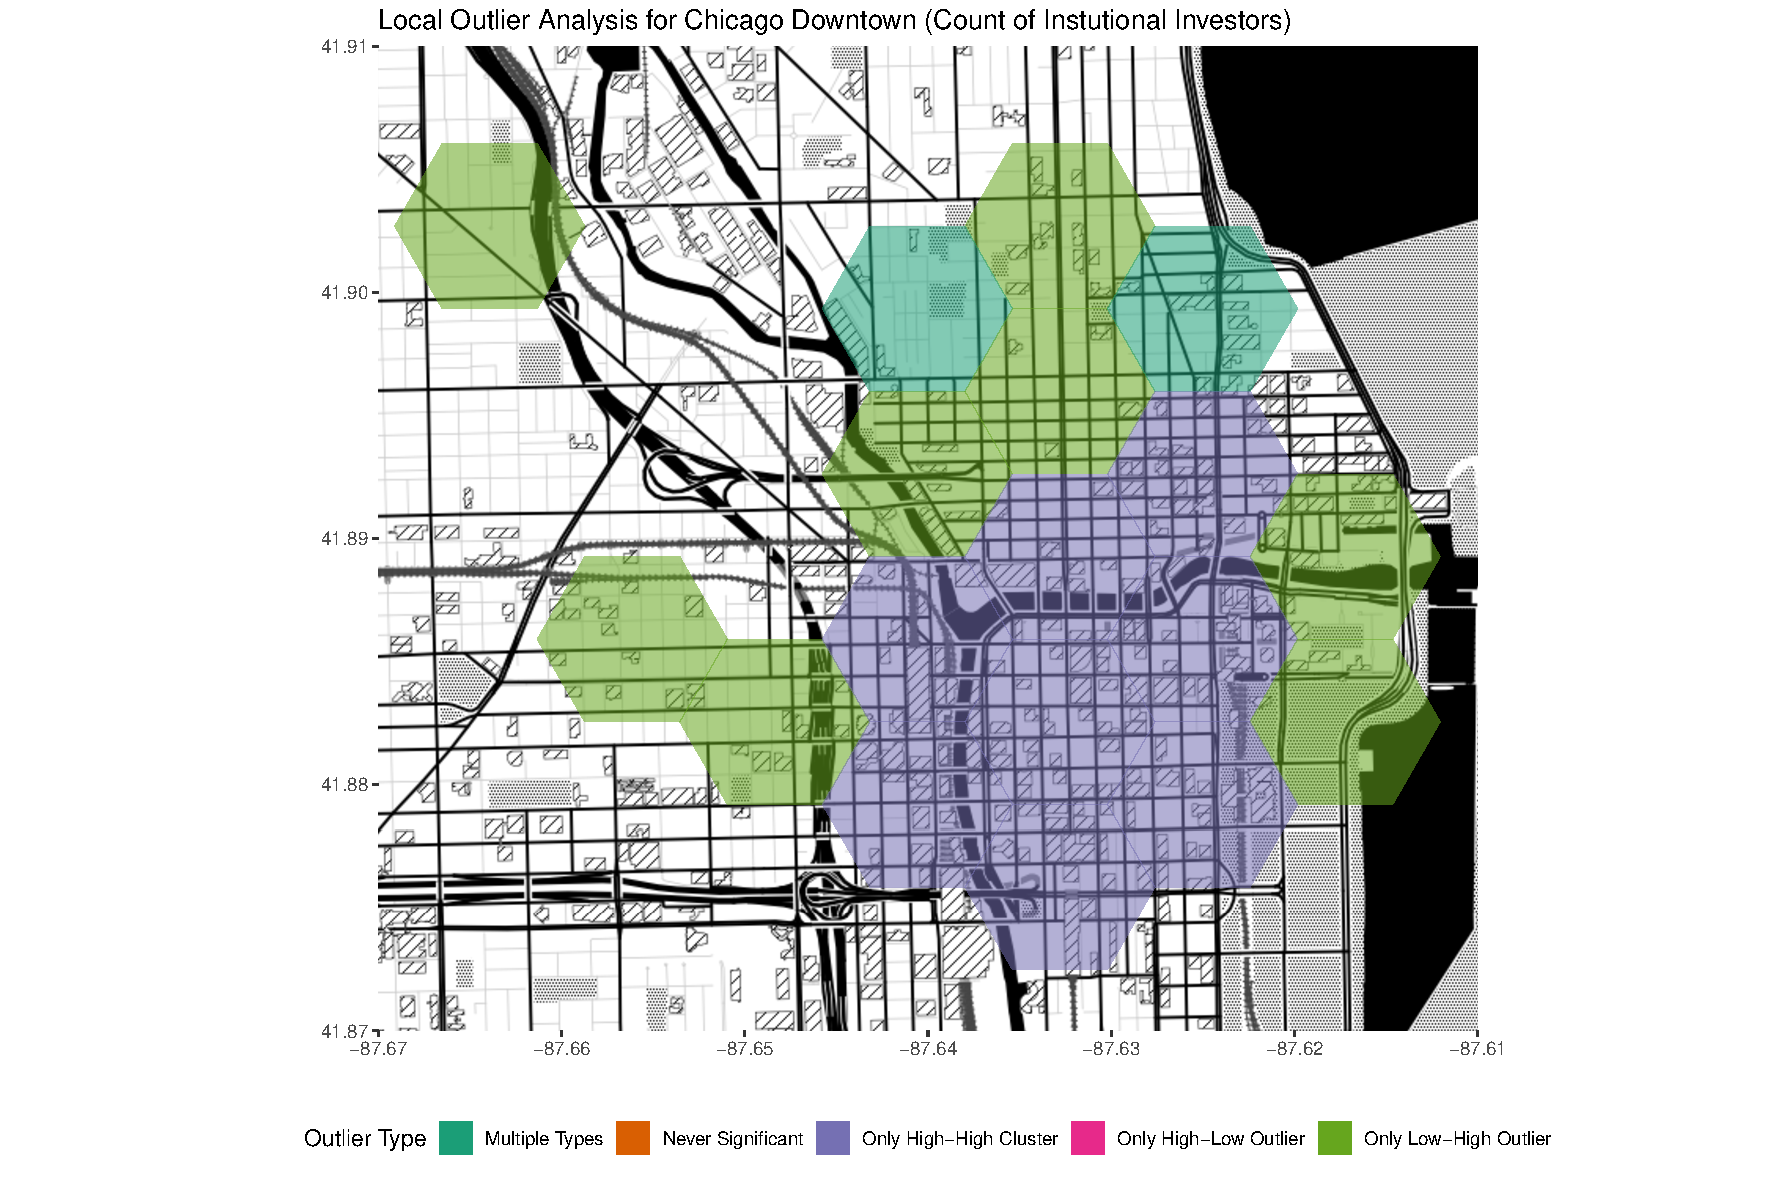
\includegraphics[width=1\linewidth]{Figures/ChapterIV/Chi_Count_LO_Downtown}
	\caption[Downtown Chicago Local Outlier Analysis - Count of Institutional Investors 1999-2018]{Chicago local outlier analysis - count of institutional investors}
	\label{fig:Chicagocountlocaloutliercount_Downtown}
\end{figure}	

\subsection{Funds Under Management}

Figure \ref{fig:Chicagonmoneyhotspot} suggests a similar picture to the other emerging hot spot analysis maps where the key variable is funds under management, for there are less regions defined as a hot spot.  In this case, the hot spots in Evanston and Highland Park disappear, and the Napierville-Aurora cluster is much smaller in size.    

\begin{figure}
	\centering
	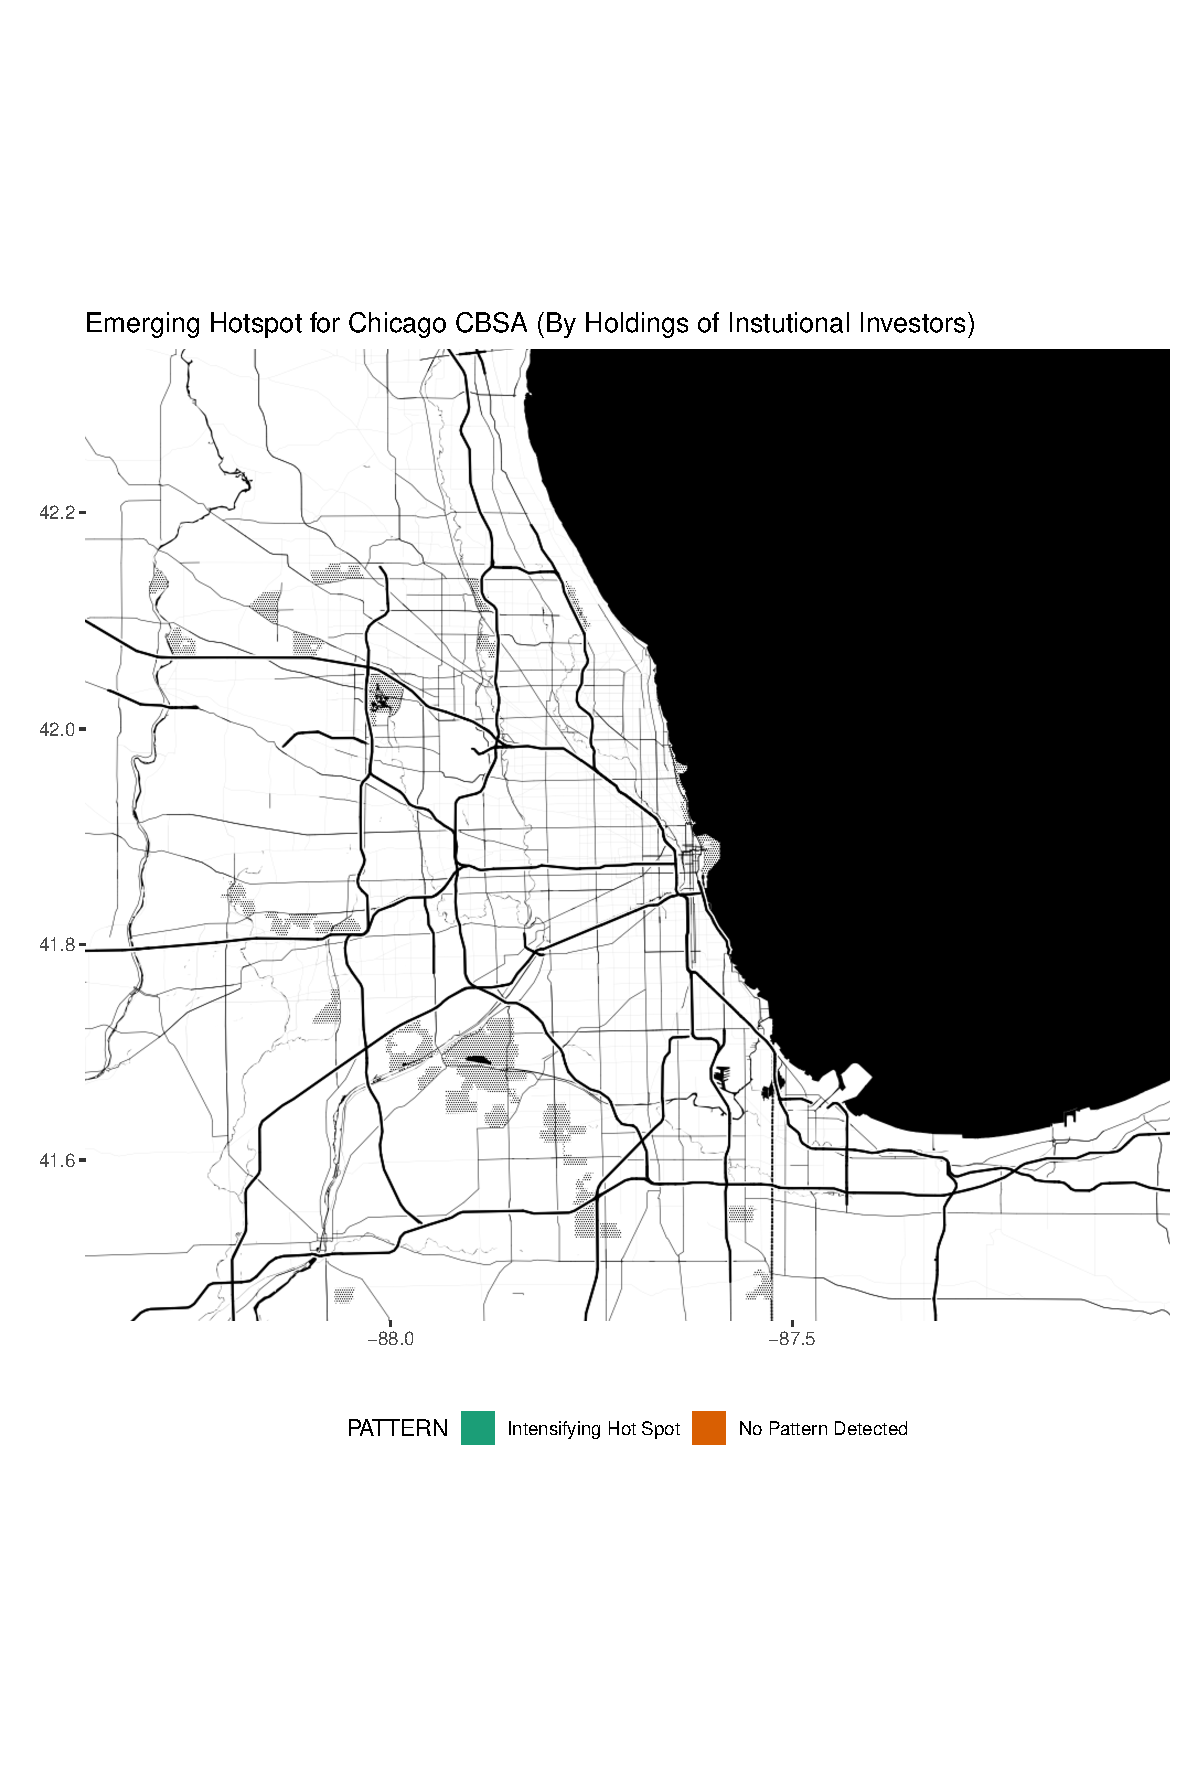
\includegraphics[width=1\linewidth]{Figures/ChapterIV/Chi_Money_EH}
	\caption[Emerging Hot Spot Analysis of Funds Under Management for Chicago CBSA 2013-2018]{Emerging hot spot analysis of funds under management for Chicago for period June 2013 to December 2018}
	\label{fig:Chicagonmoneyhotspot}
\end{figure}

\begin{figure}
	\centering
	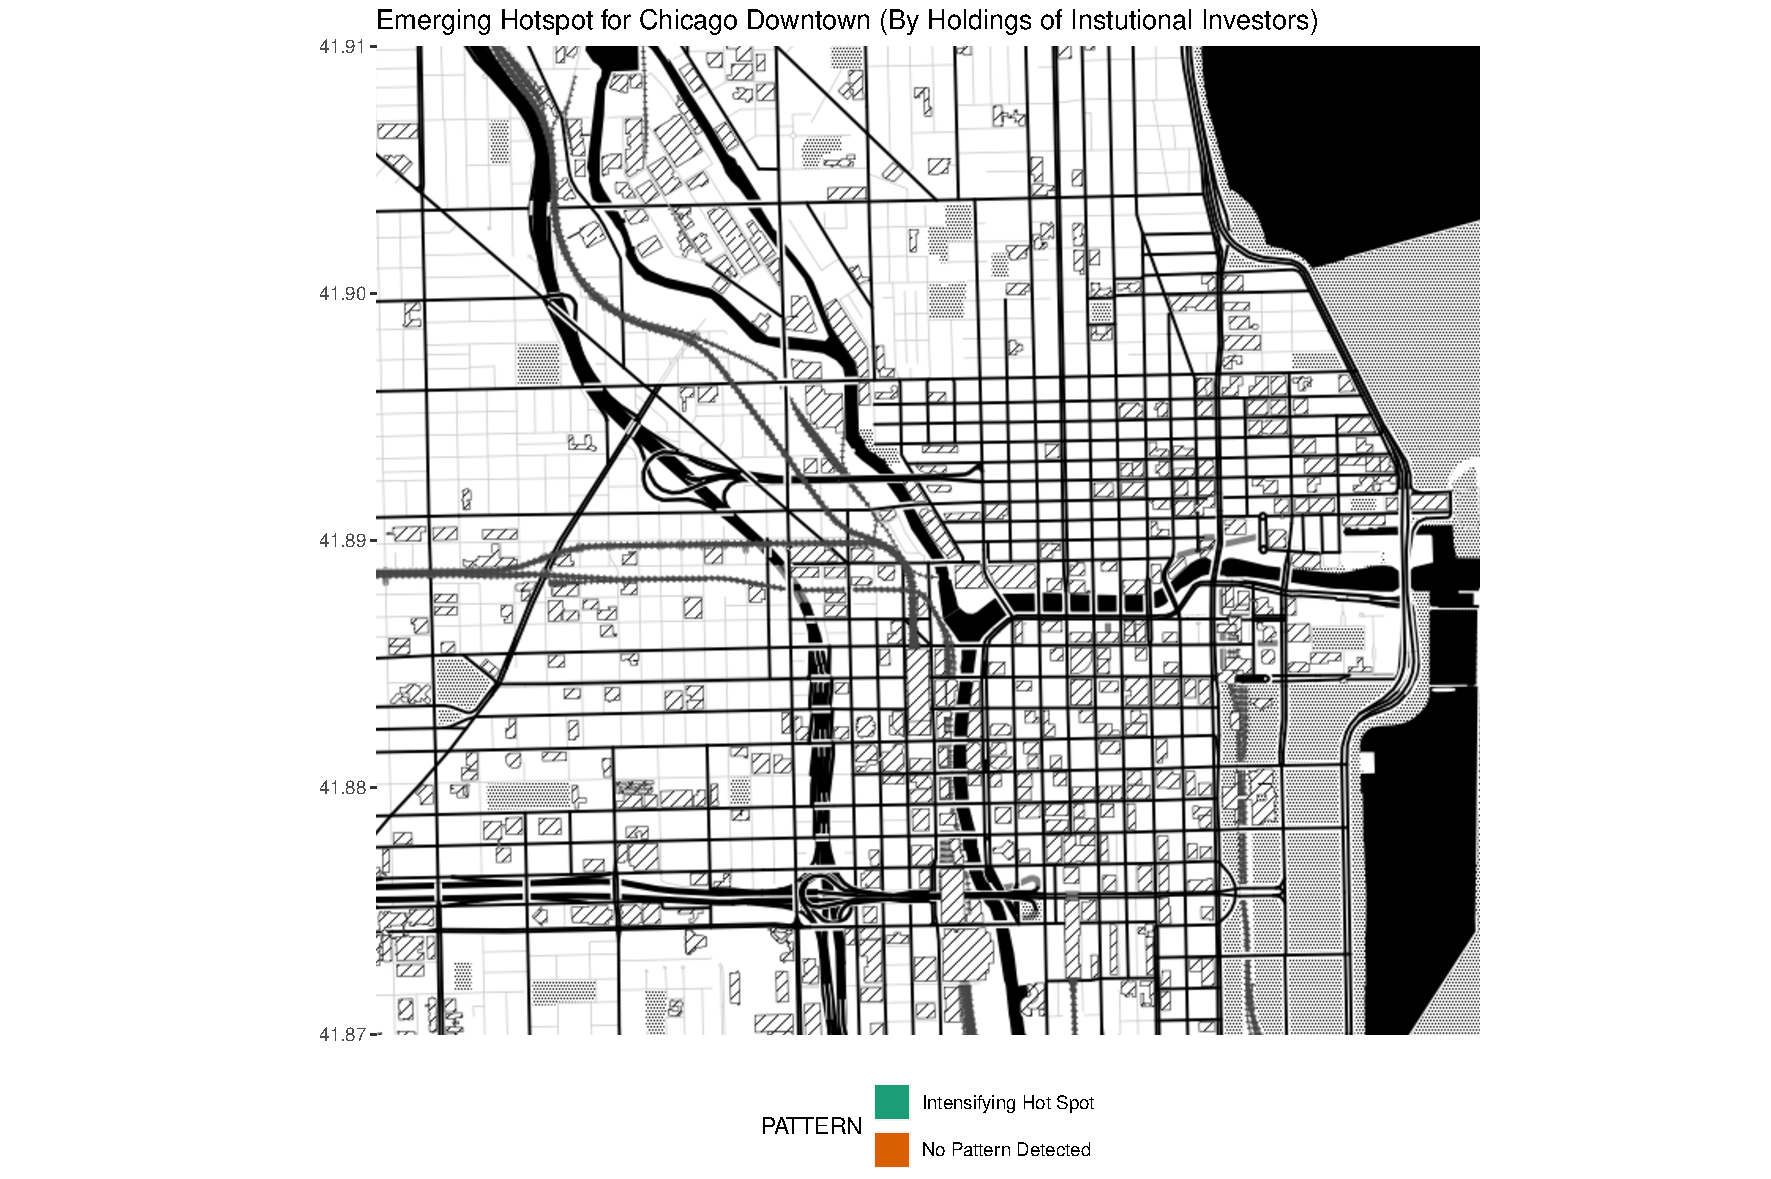
\includegraphics[width=1\linewidth]{Figures/ChapterIV/Chi_Money_EH_Downtown}
	\caption[Emerging Hot Spot Analysis of Funds Under Management for Downtown Chicago 2013-2018]{Emerging hot spot analysis of funds under management for Chicago for period June 2013 to December 2018}
	\label{fig:Chicagonmoneyhotspot_Downtown}
\end{figure}

Figure \ref{fig:Chicagolocaloutlier} paints a similar story than Figure \ref{fig:Chicagonmoneyhotspot}, for the main cluster of high-high hexagons is located in the Chicago Loop district.  A secondary cluster of a single high-high hexagon exists in the Napierville-Aurora region.  Furthermore, the cluster in the Loop neighbourhood of Chicago is much more defined in this analysis compared to the count map. This sharper cluster is not surprising considering the presence of the Chicago financial district, anchored by the Chicago Mercantile Exchange, at the centre of the Loop.


\begin{figure}
	\centering
	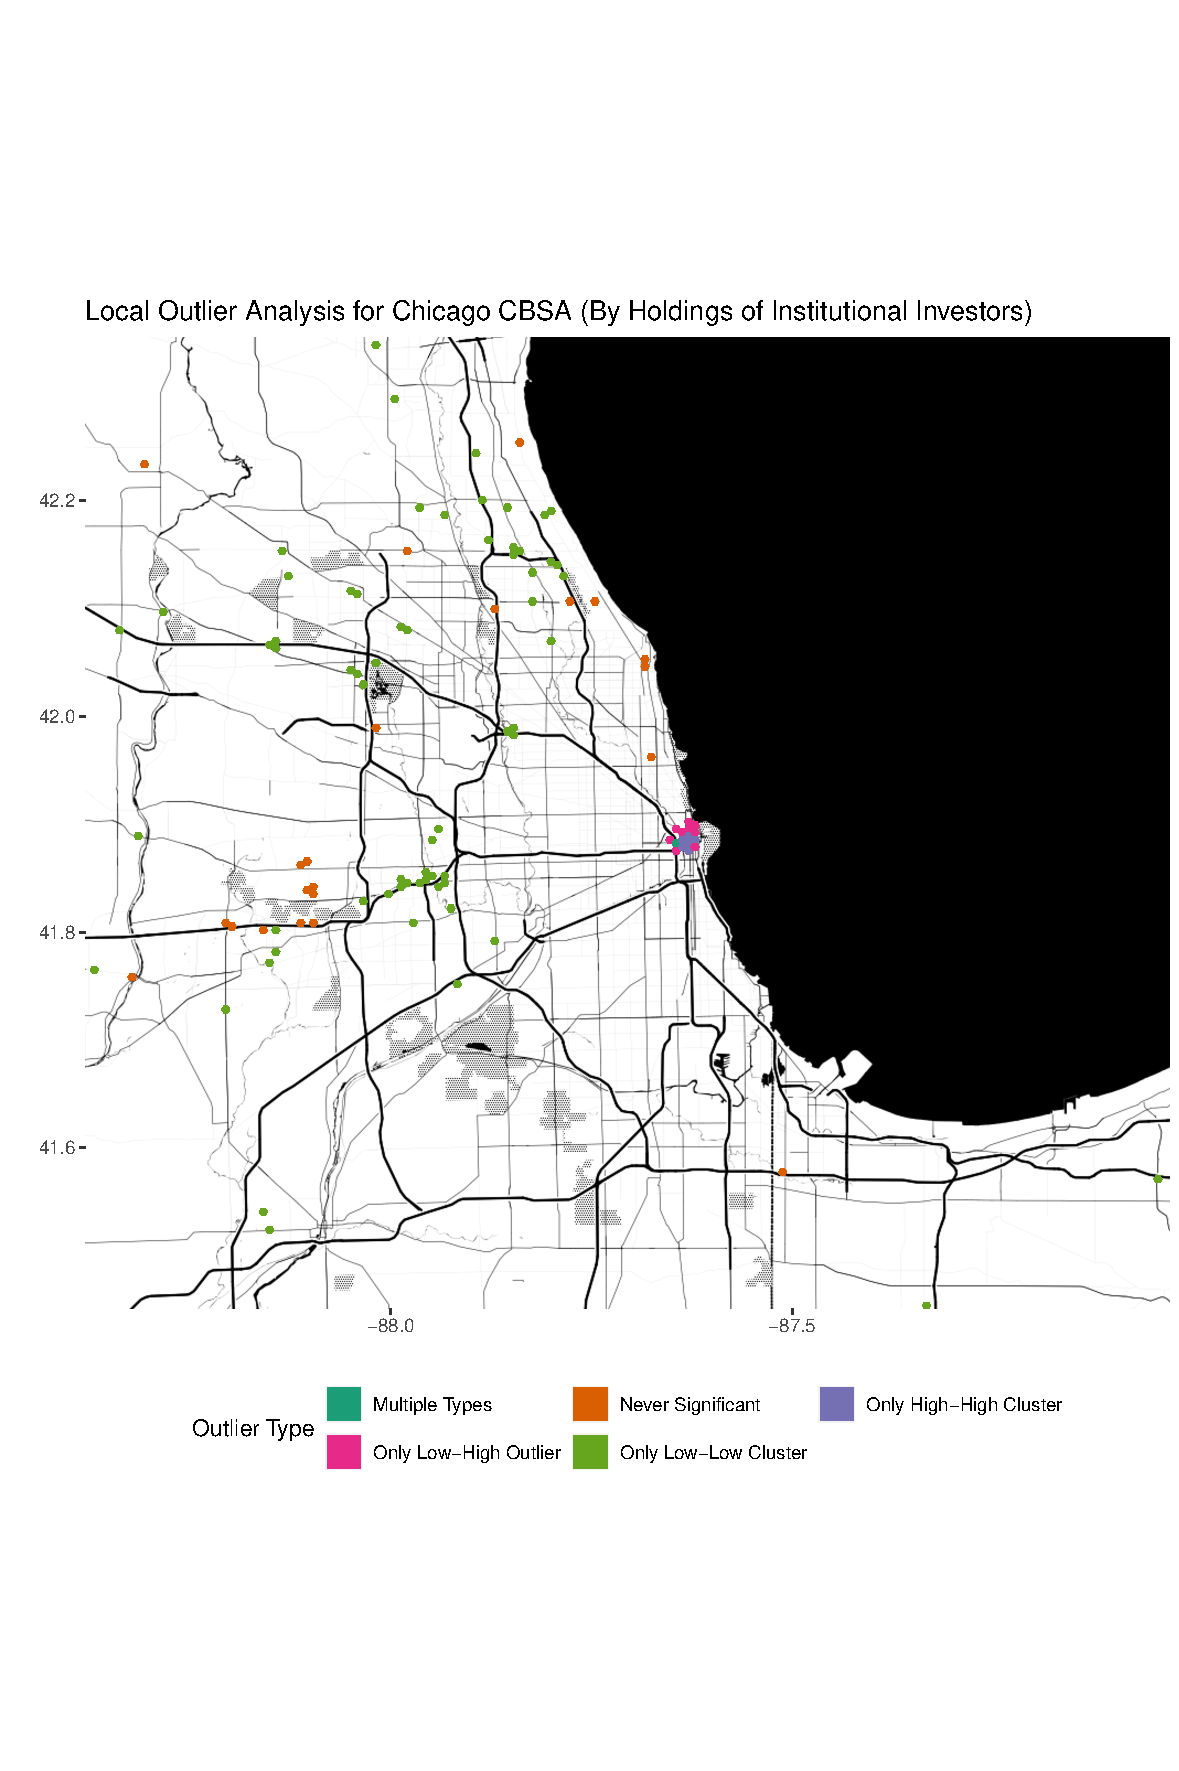
\includegraphics[width=1\linewidth]{Figures/ChapterIV/Chi_Money_LO}
	\caption[Chicago CBSA Local Outlier Analysis - Funds Under Management 2013-2018]{Chicago local outlier analysis - funds under management}
	\label{fig:Chicagolocaloutlier}
\end{figure}


\begin{figure}
	\centering
	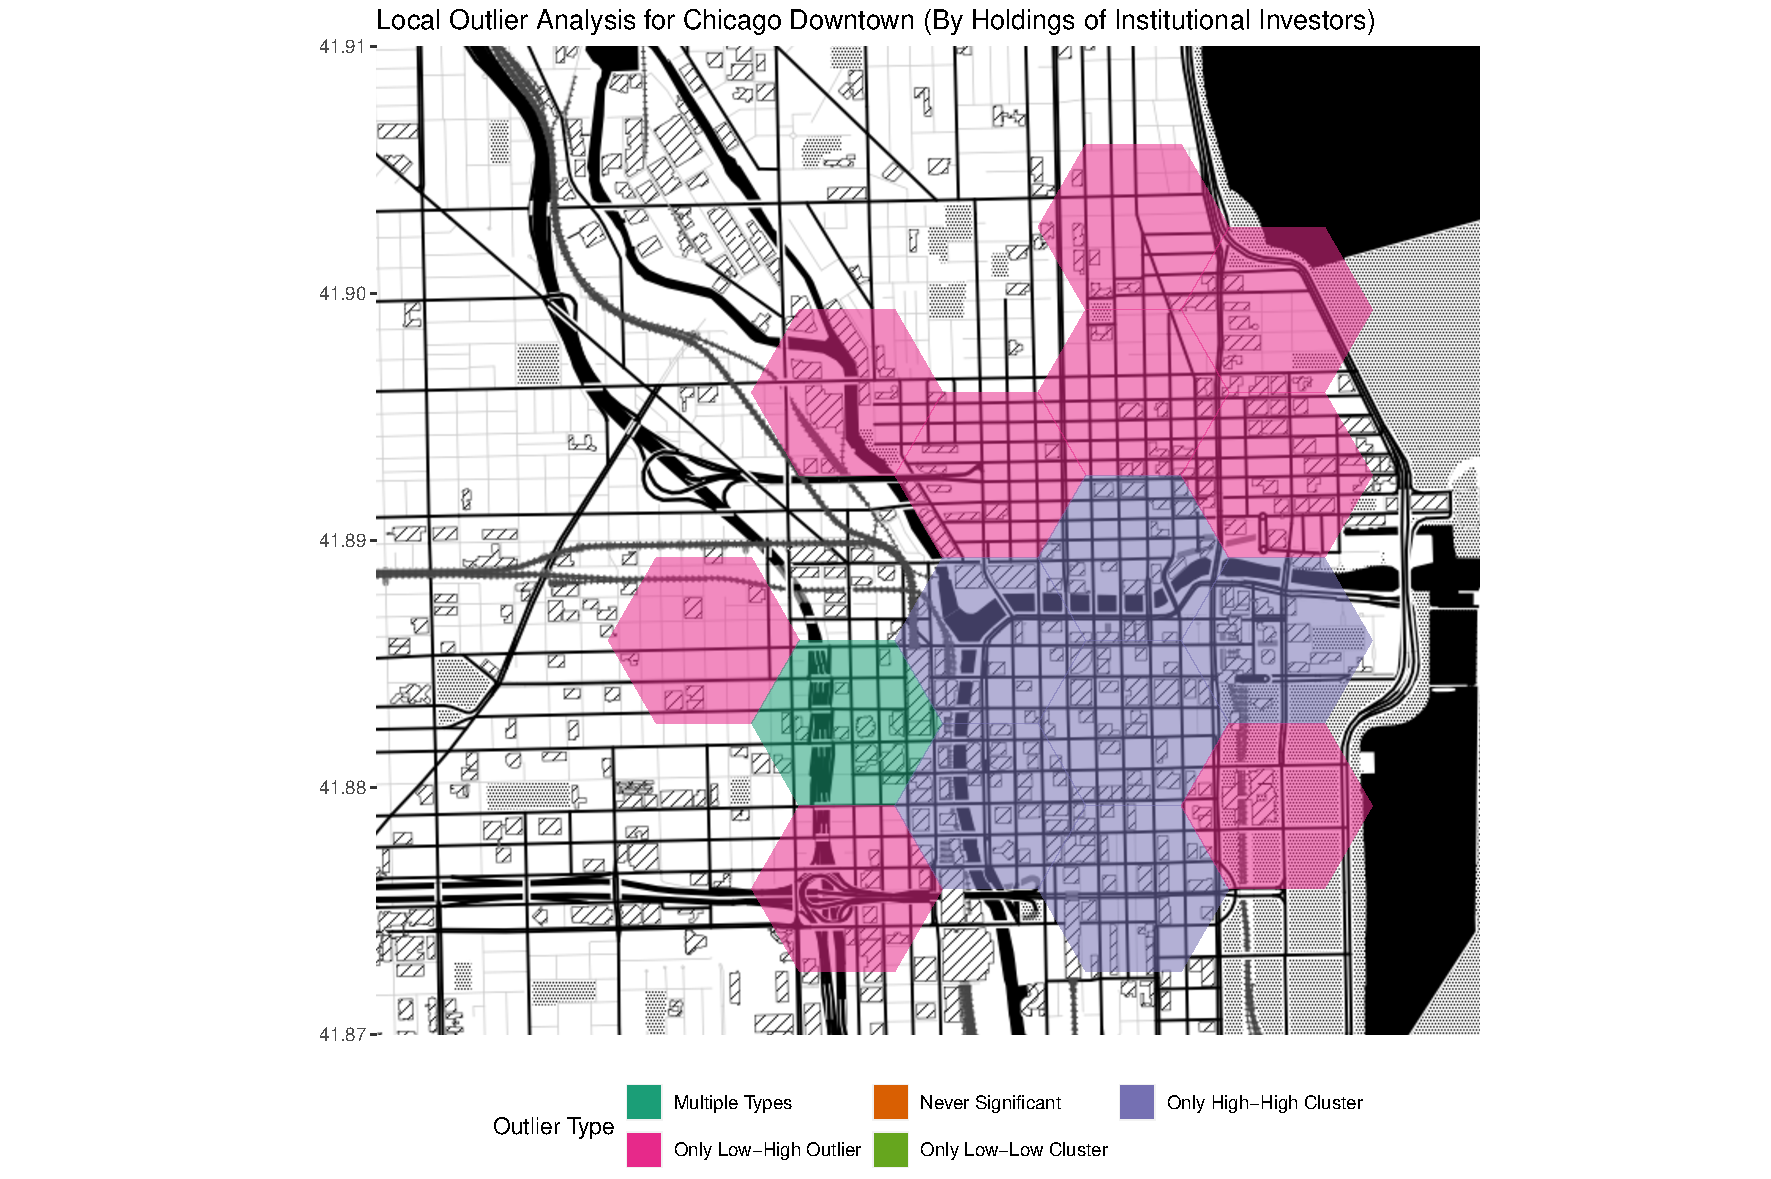
\includegraphics[width=1\linewidth]{Figures/ChapterIV/Chi_Money_LO_Downtown}
	\caption[Downtown Chicago Local Outlier Analysis - Funds Under Management 2013-2018]{Chicago local outlier analysis - funds under management}
	\label{fig:Chicagolocaloutlier_Downtown}
\end{figure}

\section{Los Angeles}



\subsection{Count Data}

Figure \ref{fig:LAcounthotspot} indicates that there is an absence of a central financial district and that investors are more diffused.	As such, unlike Boston and Chicago, the emerging hot spot analysis map for Los Angeles offers more categories.  This broad spread of hot spots is not really surprising considering Los Angeles's history and reputation for urban sprawl and suburban office parks \citep{dearpostmodern1998,harrisconstructing1998}.  The lack of a historic CBD comprised of skyscrapers on the scale of New York's Wall Street and Midtown or Chicago's Loop district and decentralized city administration certainly help in creating multiple small intensifying hot spots around the city such as Downtown, Santa Monica, Beverly Hills, Costa Mesa and Irvine. 

These hot spot locations also show up in Figure \ref{fig:LAcountlocaloutliercount} as local outliers.  However, there is a large amount of hexagons displaying the mixed outlier type in Santa Monica.  This can be partially explained by the diffuse nature of locations in Santa Monica compared to other clusters such that across time they might appear as high-highs or high-lows due to neighbourhood effects.  

\begin{figure}
	\centering
	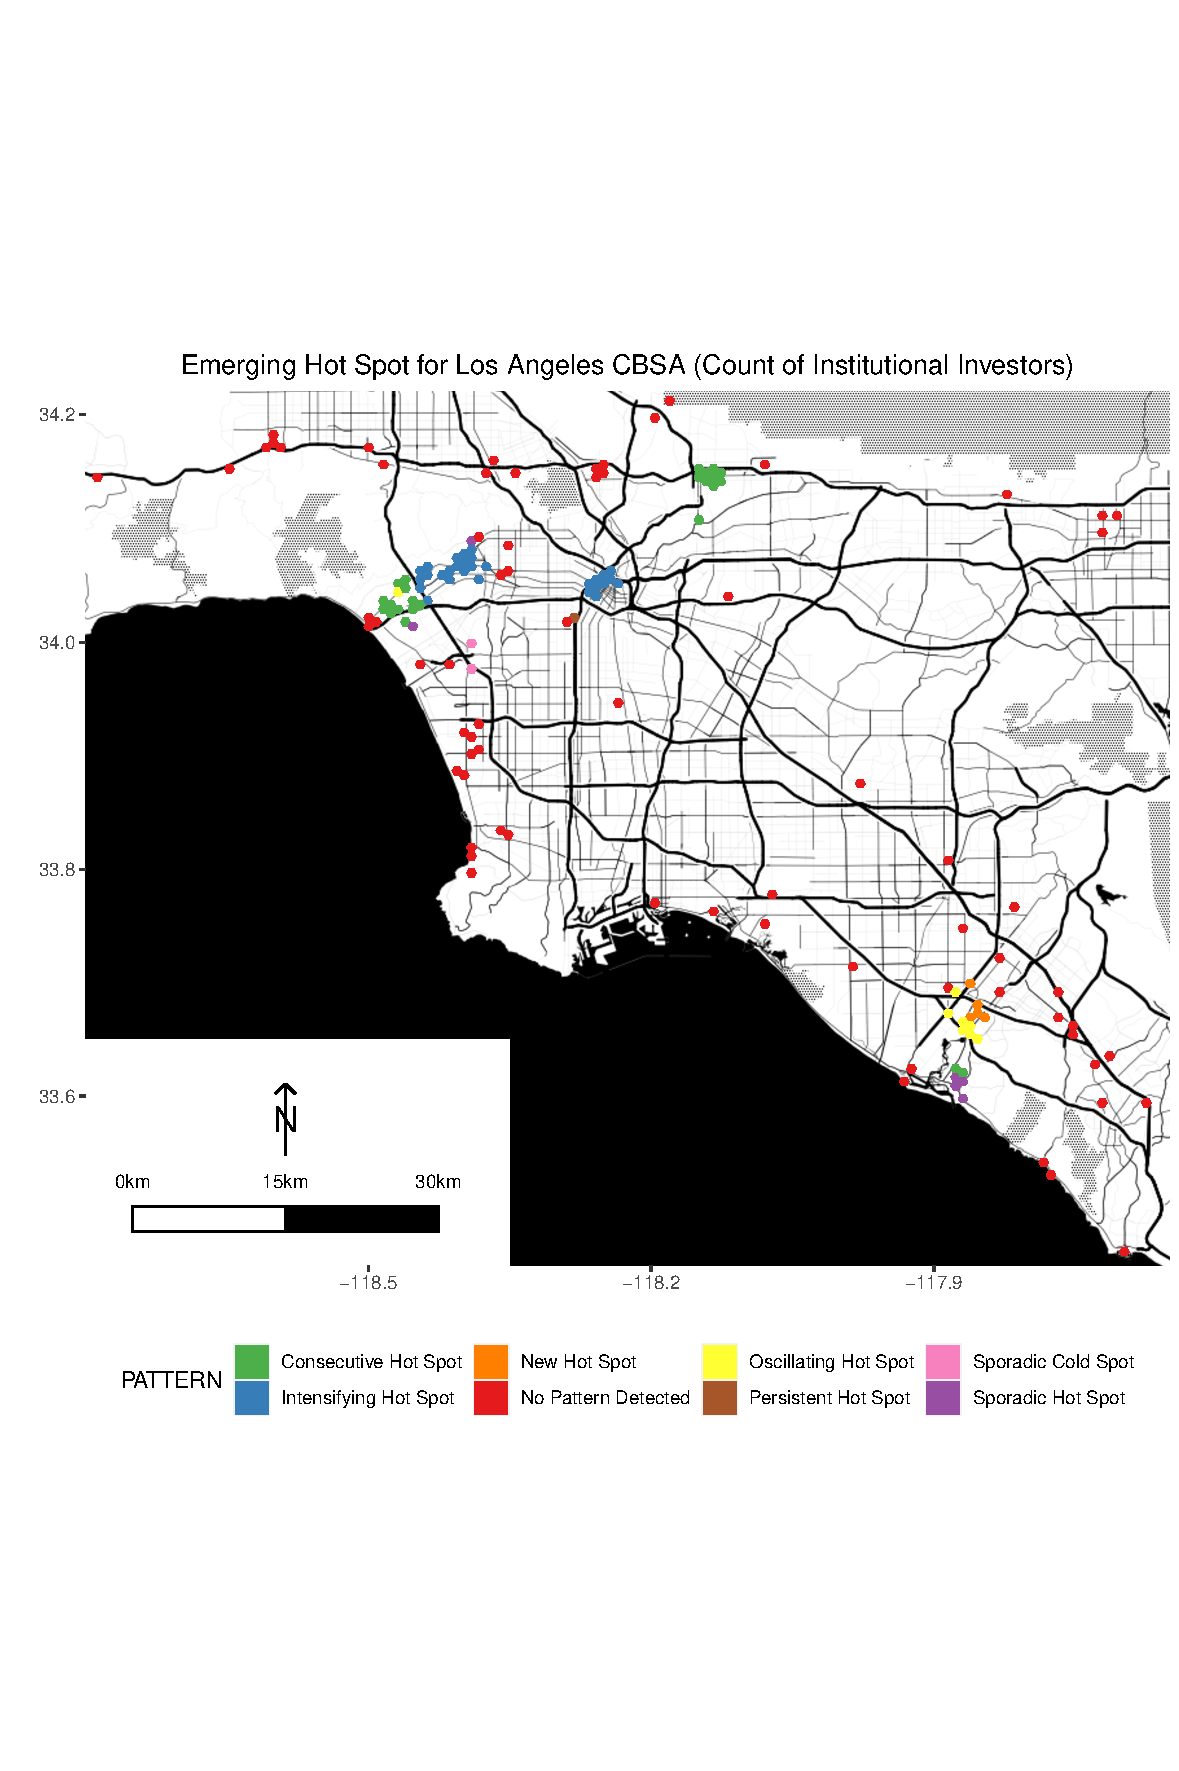
\includegraphics[width=1\linewidth]{Figures/ChapterIV/LA_Count_EH}
	\caption[Hot Spot Analysis of Number of Firms in Los Angeles CBSA 1999-2018]{Hot spot analysis of number of firms in Los Angeles for the time period March 1999 to December 2018}
	\label{fig:LAcounthotspot}
\end{figure}

\begin{figure}
	\centering
	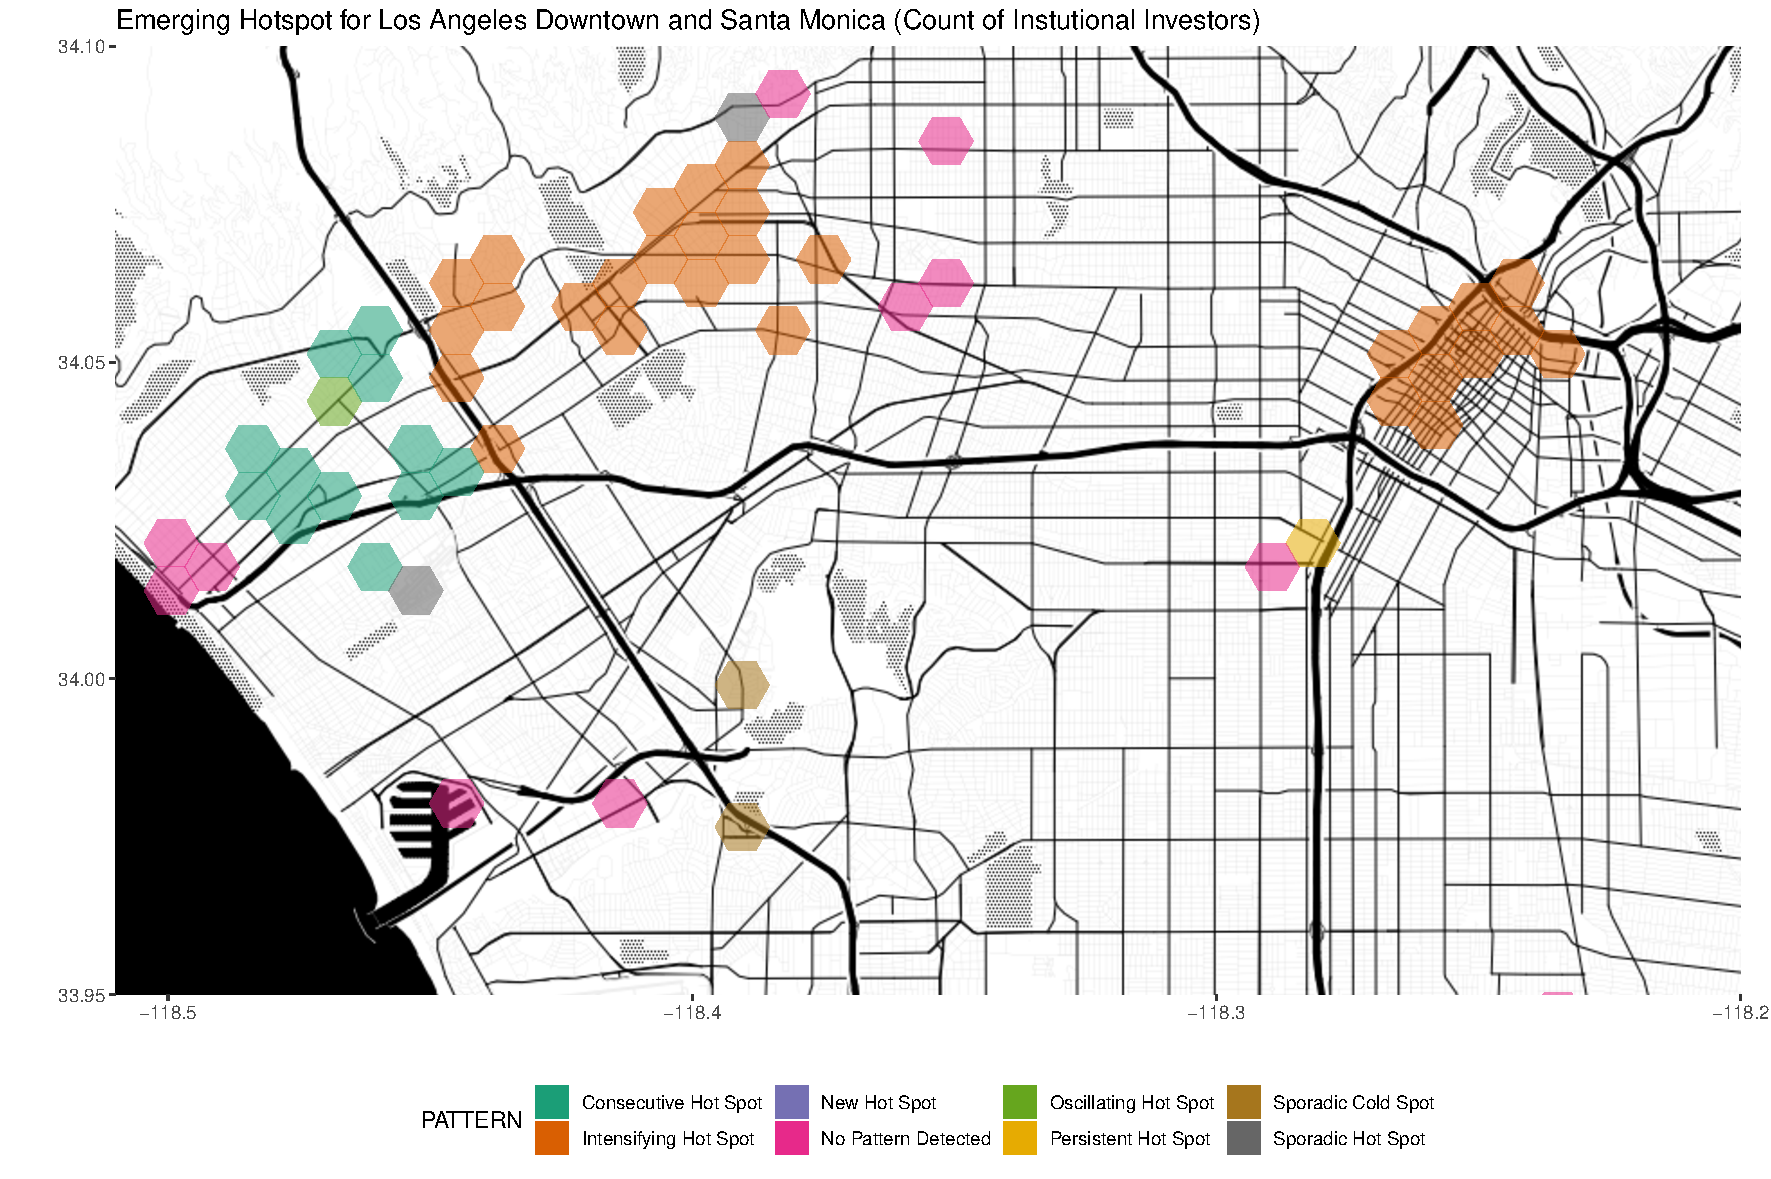
\includegraphics[width=1\linewidth]{Figures/ChapterIV/LA_Count_EH_Downtown}
	\caption[Hot Spot Analysis of Number of Firms in Downtown Los Angeles and Santa Monica 1999-2018]{Hot spot analysis of number of firms in downtown Los Angeles and Santa Monica for the time period March 1999 to December 2018}
	\label{fig:LAcounthotspot_Downtown}
\end{figure}


\begin{figure}
	\centering
	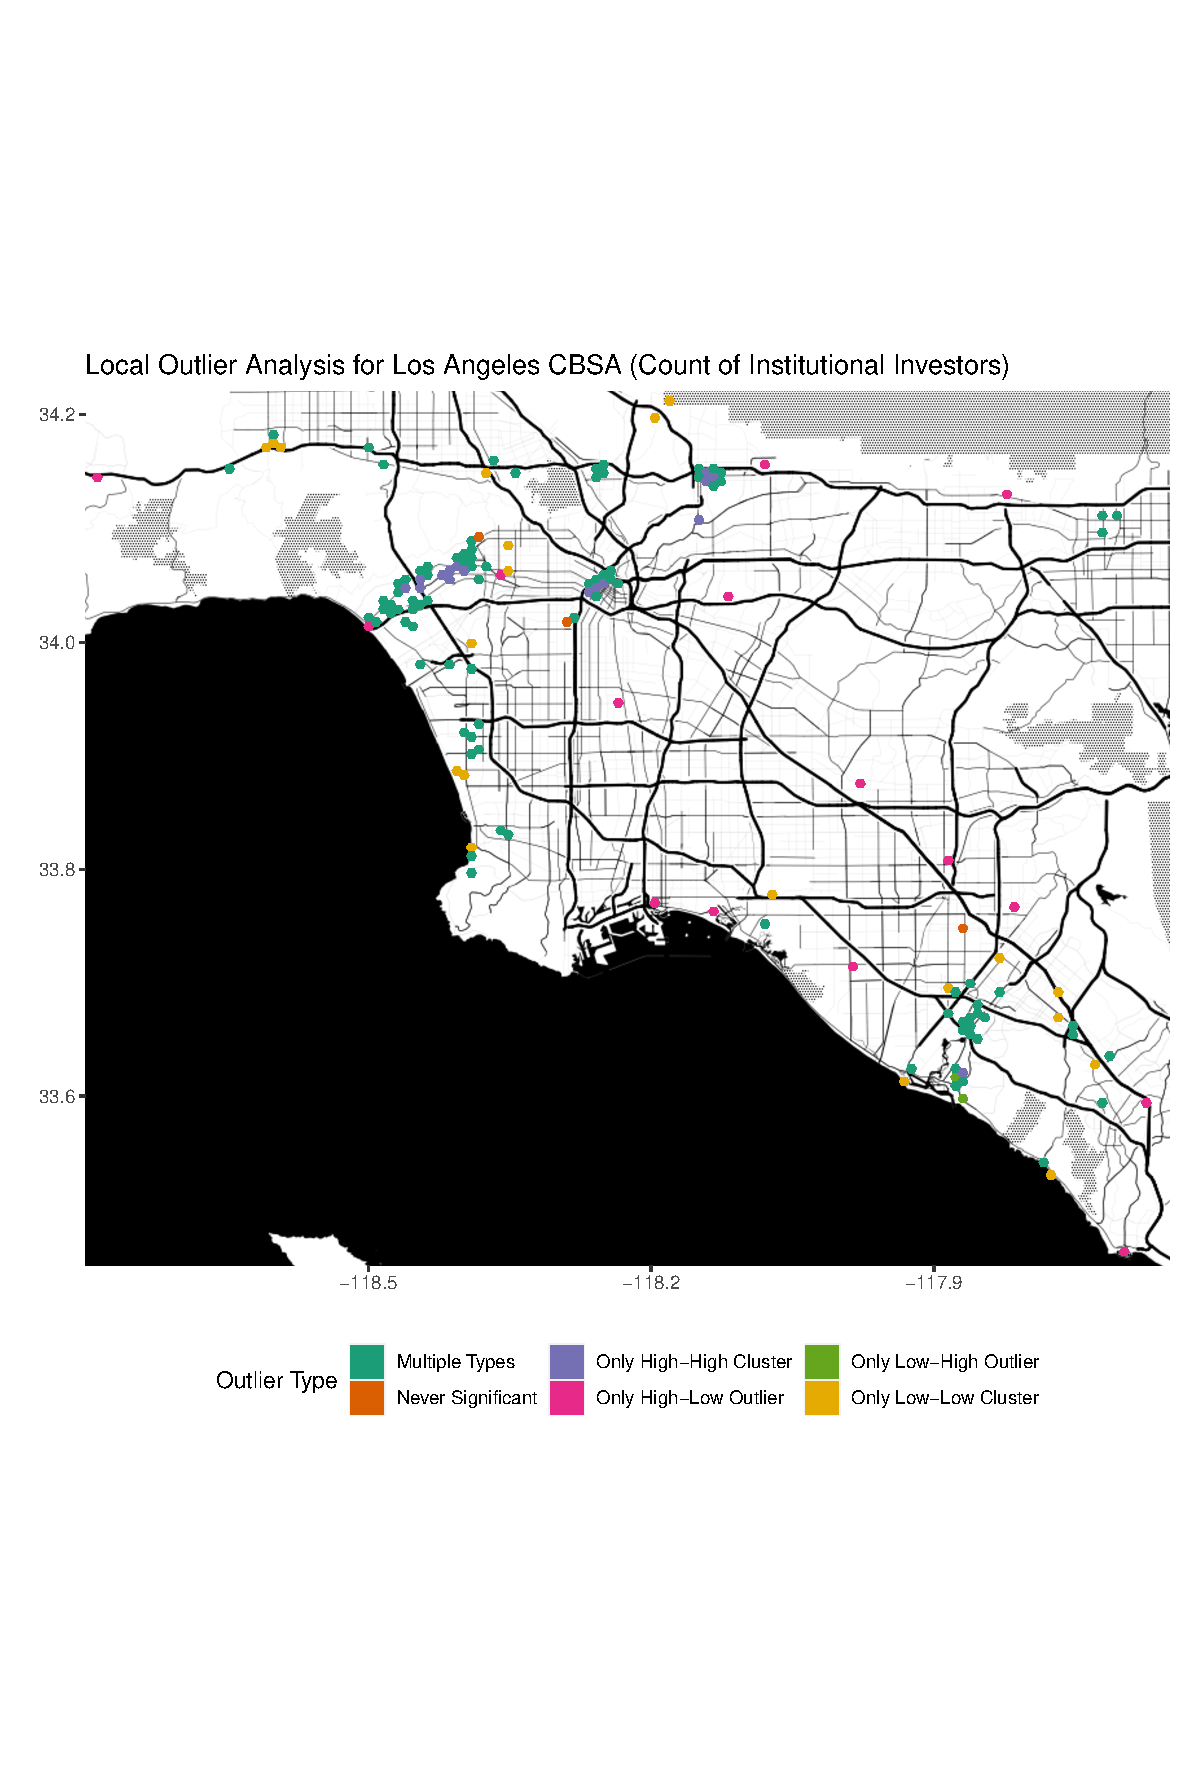
\includegraphics[width=1\linewidth]{Figures/ChapterIV/LA_Count_LO}
	\caption[Los Angeles CBSA Local Outlier Analysis - Count of Institutional Investors 1999-2018]{Los Angeles local outlier analysis - count of institutional investors}
	\label{fig:LAcountlocaloutliercount}
\end{figure}	

\begin{figure}
	\centering
	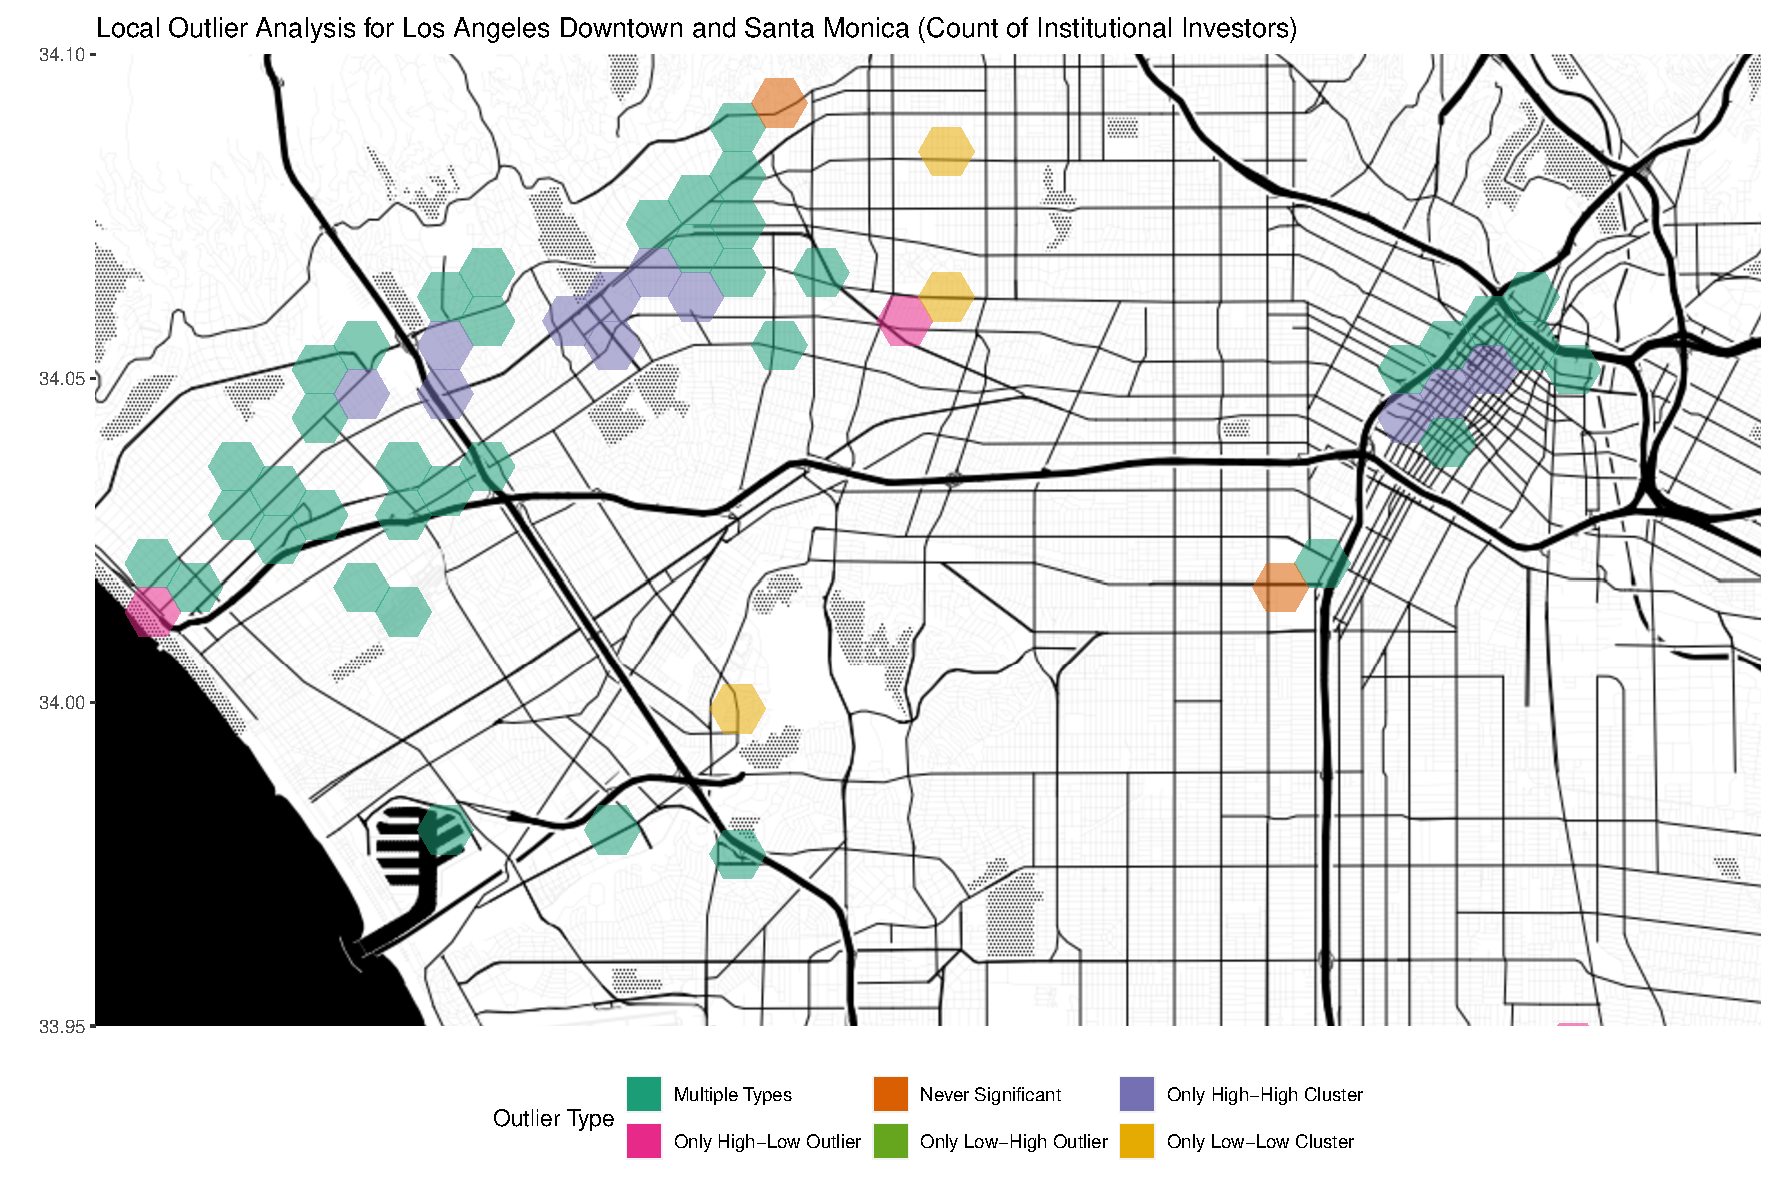
\includegraphics[width=1\linewidth]{Figures/ChapterIV/LA_Count_LO_Downtown}
	\caption[Downtown Los Angeles and Santa Monica Local Outlier Analysis - Count of Institutional Investors 1999-2018]{Downtown Los Angeles and Santa Monica local outlier analysis - count of institutional investors}
	\label{fig:LAcountlocaloutliercount_Downtown}
\end{figure}	

\subsection{Funds Under Management}

Continuing the theme seen in all previous maps with regards to analysing funds under management, the map that is weighted by money rather then the mere presence of an investor reduces the importance of suburban investors.  This suggests that while suburban investors are becoming more common, their portfolio of holdings are smaller than CBD-based investors.  

The emerging hot spot analysis for Figure \ref{fig:LAmoneyhotspot} as well as the local outlier analysis in Figure \ref{fig:LAlocaloutlier} drops the Costa Mesa  and Irvine hot spots.  Furthermore, the Downtown Los Angeles hot spot remains the only one that is still an intensifying hot spot.  This can be explained by the recent construction boom in high grade office towers being built in the Downtown after an influx of foreign capital and a planning mandate towards densification \citep{Marino19}.  


\begin{figure}
	\centering
	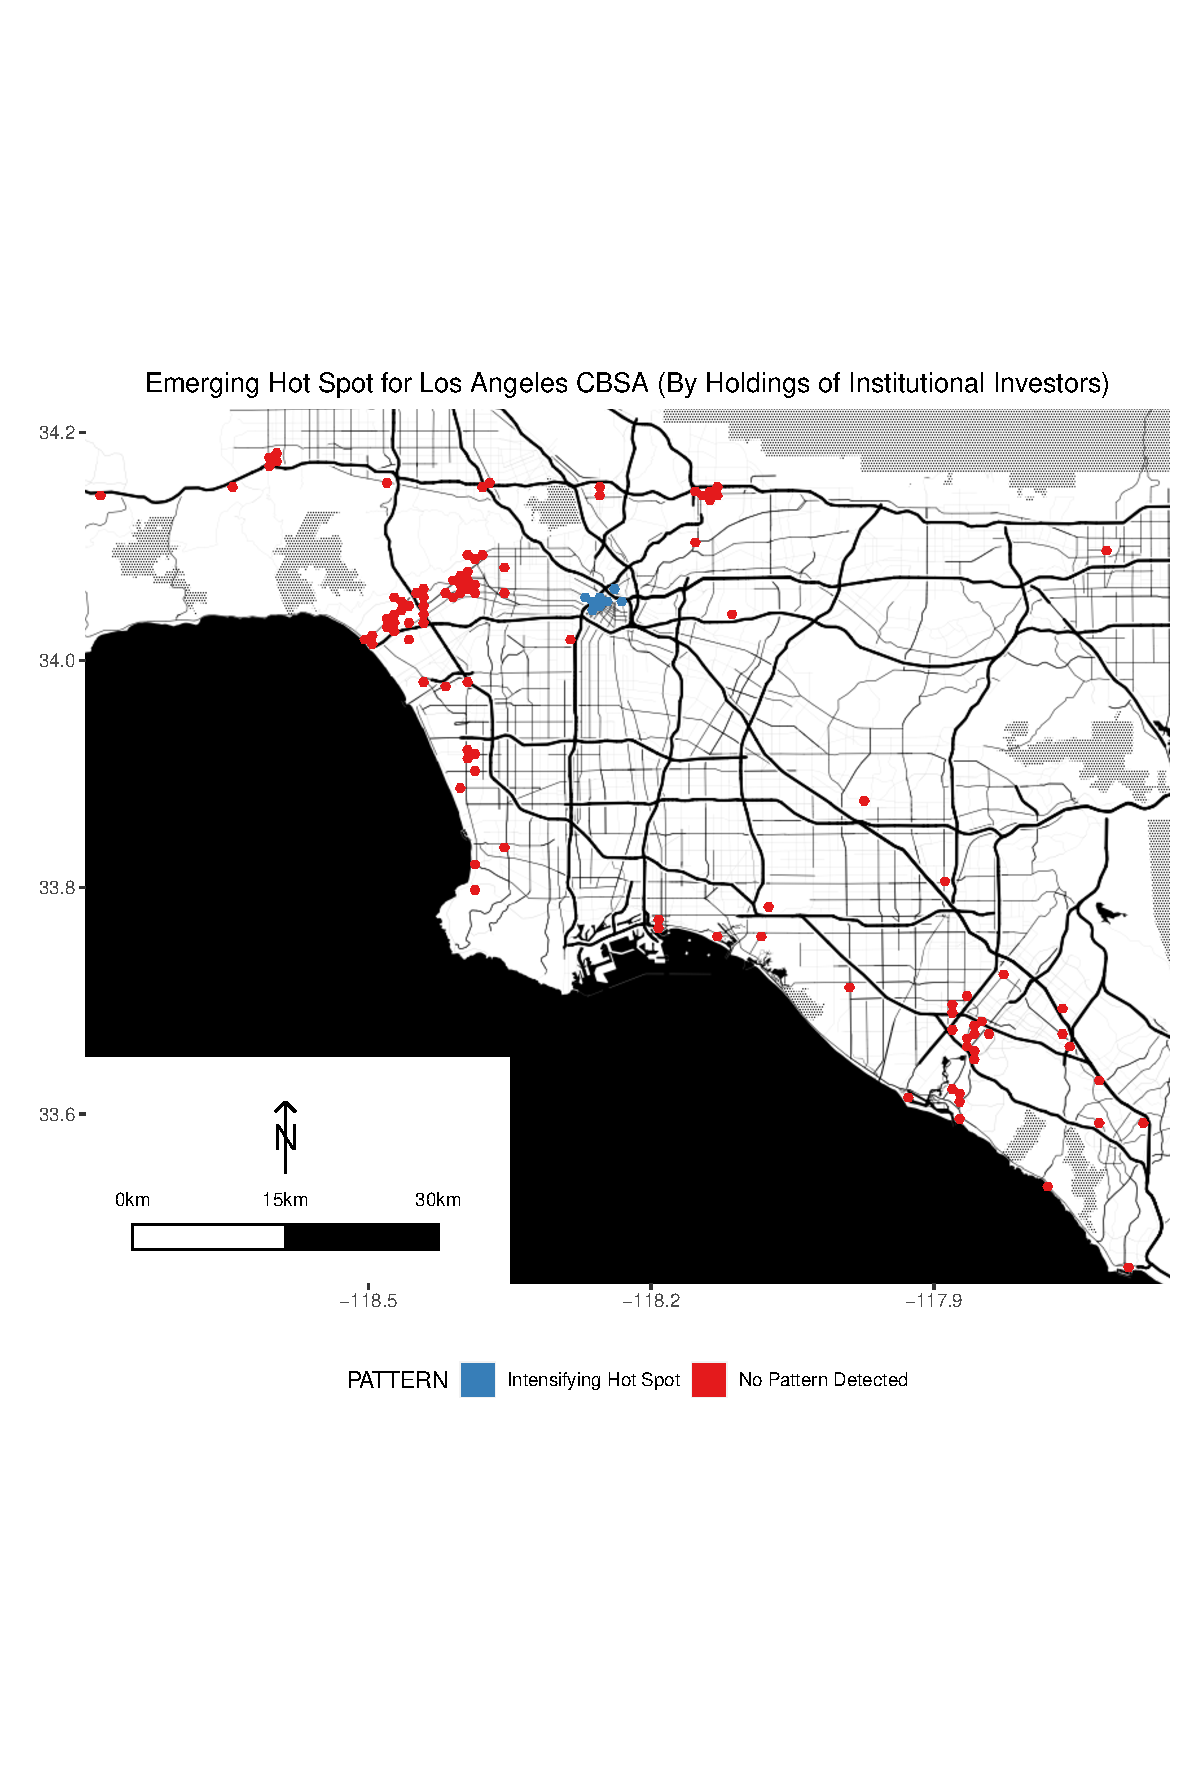
\includegraphics[width=1\linewidth]{Figures/ChapterIV/LA_Money_EH}
	\caption[Emerging Hot Spot Analysis of Funds Under Management for Los Angeles CBSA 2013-2018]{Emerging hot spot analysis of funds under management for Los Angeles for period June 2013 to December 2018}
	\label{fig:LAmoneyhotspot}
\end{figure}

\begin{figure}
	\centering
	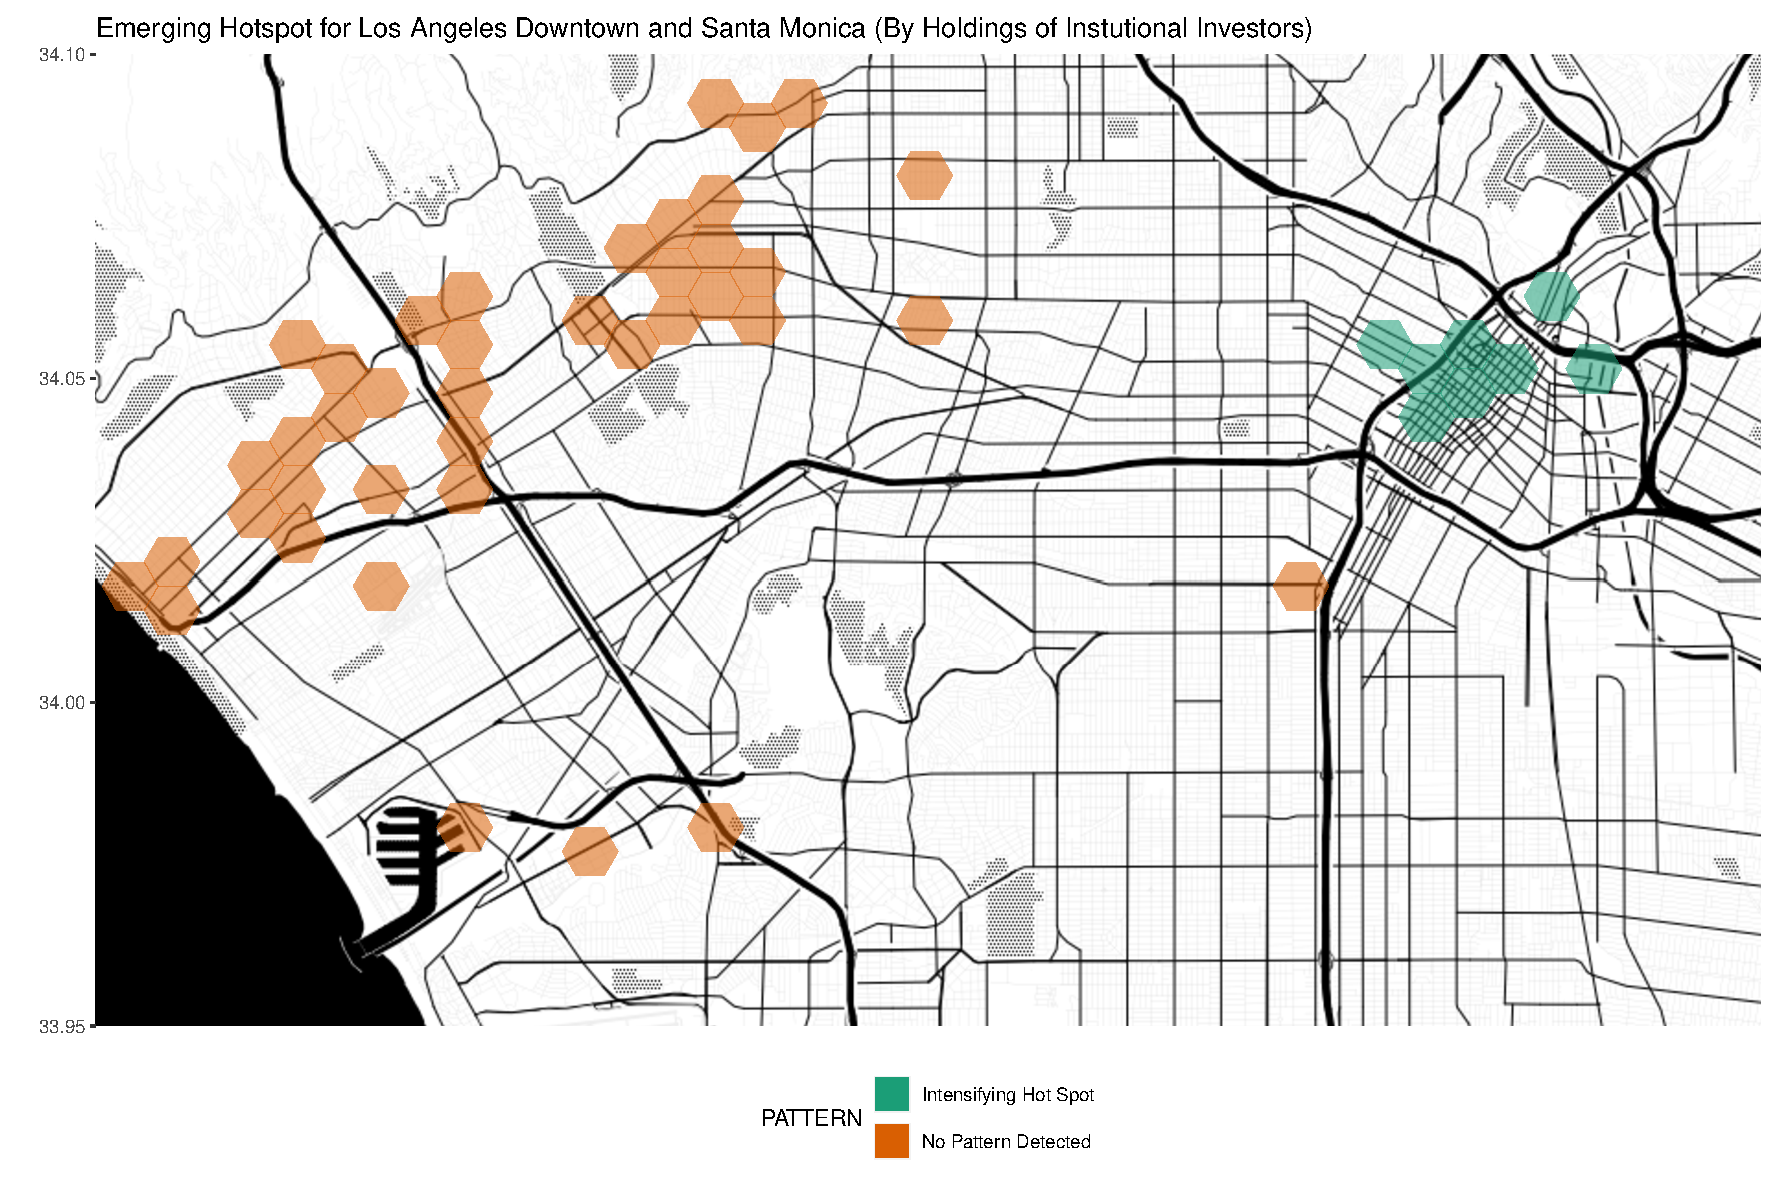
\includegraphics[width=1\linewidth]{Figures/ChapterIV/LA_Money_EH_Downtown}
	\caption[Emerging Hot Spot Analysis of Funds Under Management for Downtown Los Angeles and Santa Monica 2013-2018]{Emerging hot spot analysis of funds under management for downtown Los Angeles and Santa Monica for period June 2013 to December 2018}
	\label{fig:LAmoneyhotspot_Downtown}
\end{figure}

\begin{figure}
	\centering
	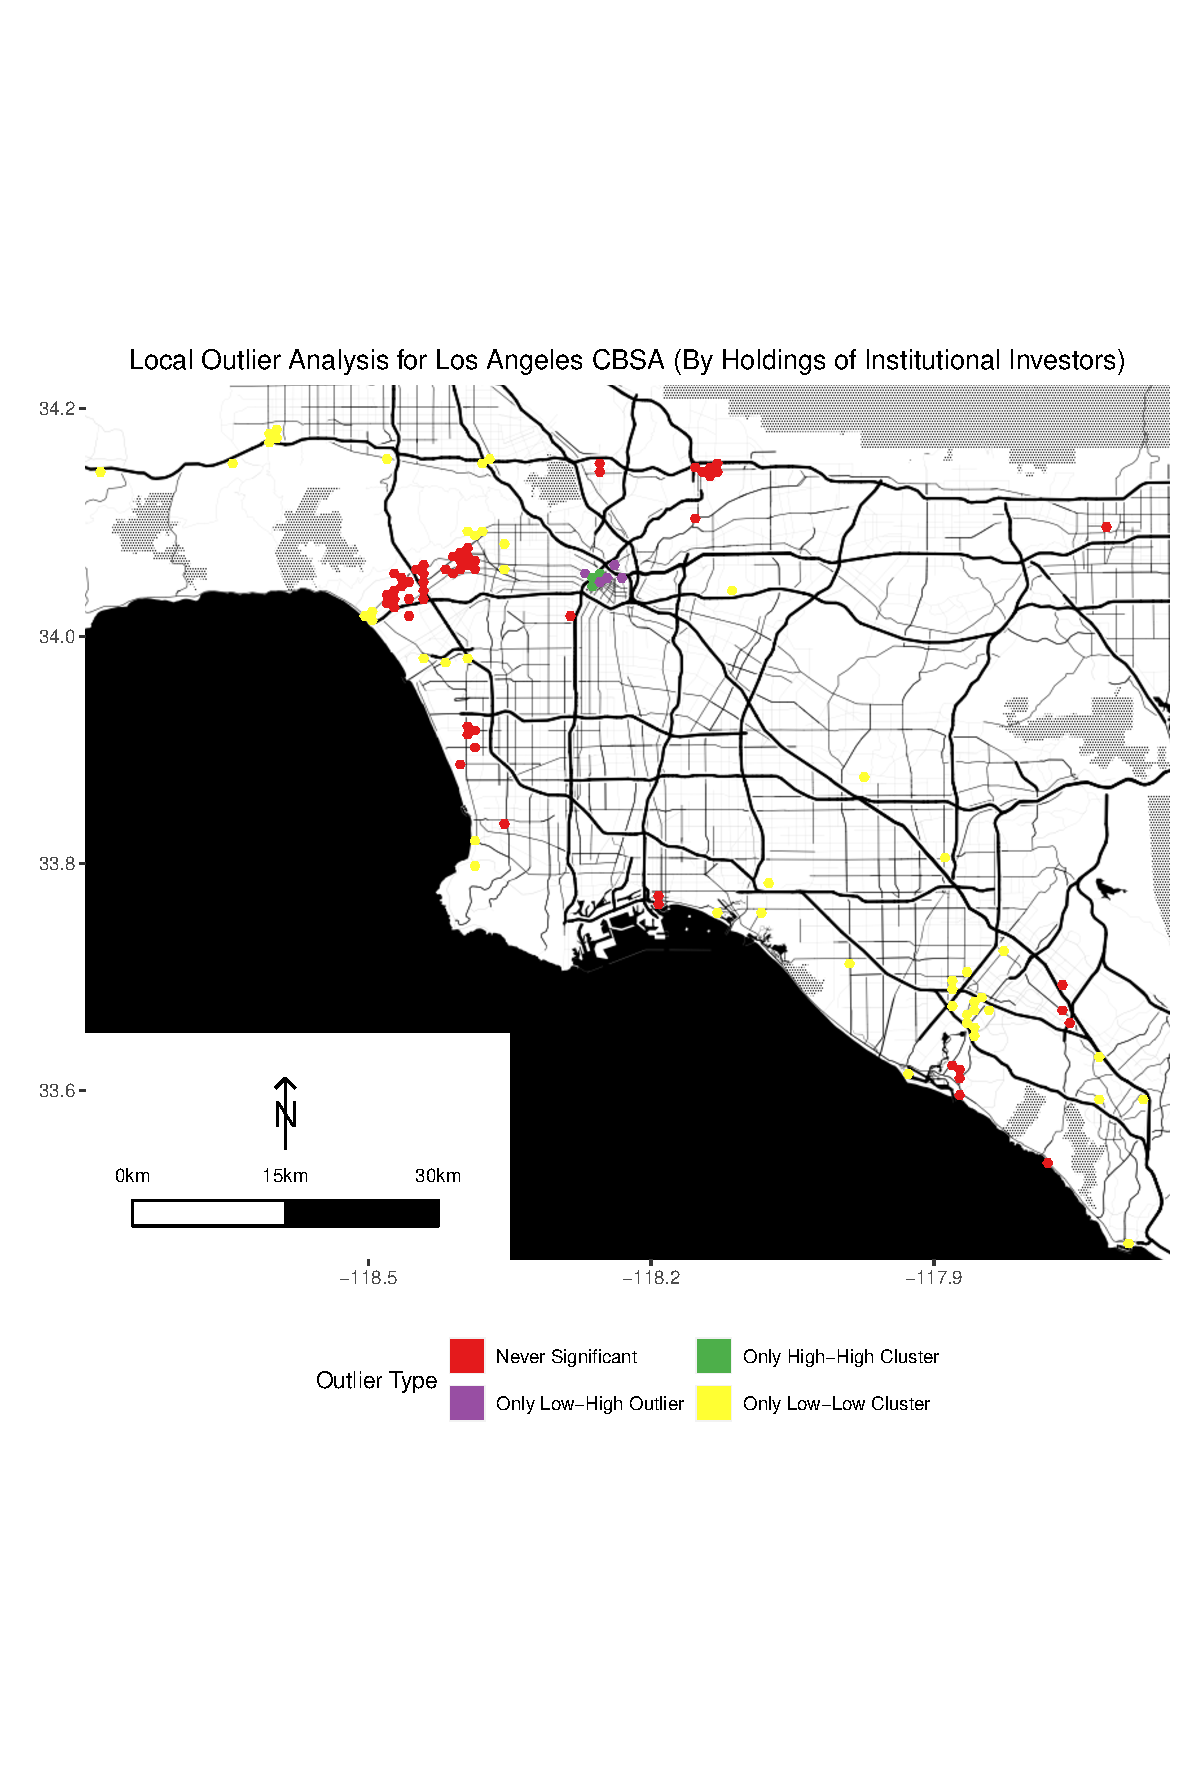
\includegraphics[width=1\linewidth]{Figures/ChapterIV/LA_Money_LO}
	\caption[Los Angeles CBSA Local Outlier Analysis - Funds Under Management 2013-2018]{Los Angeles local outlier analysis - funds under management}
	\label{fig:LAlocaloutlier}
\end{figure}

\begin{figure}
	\centering
	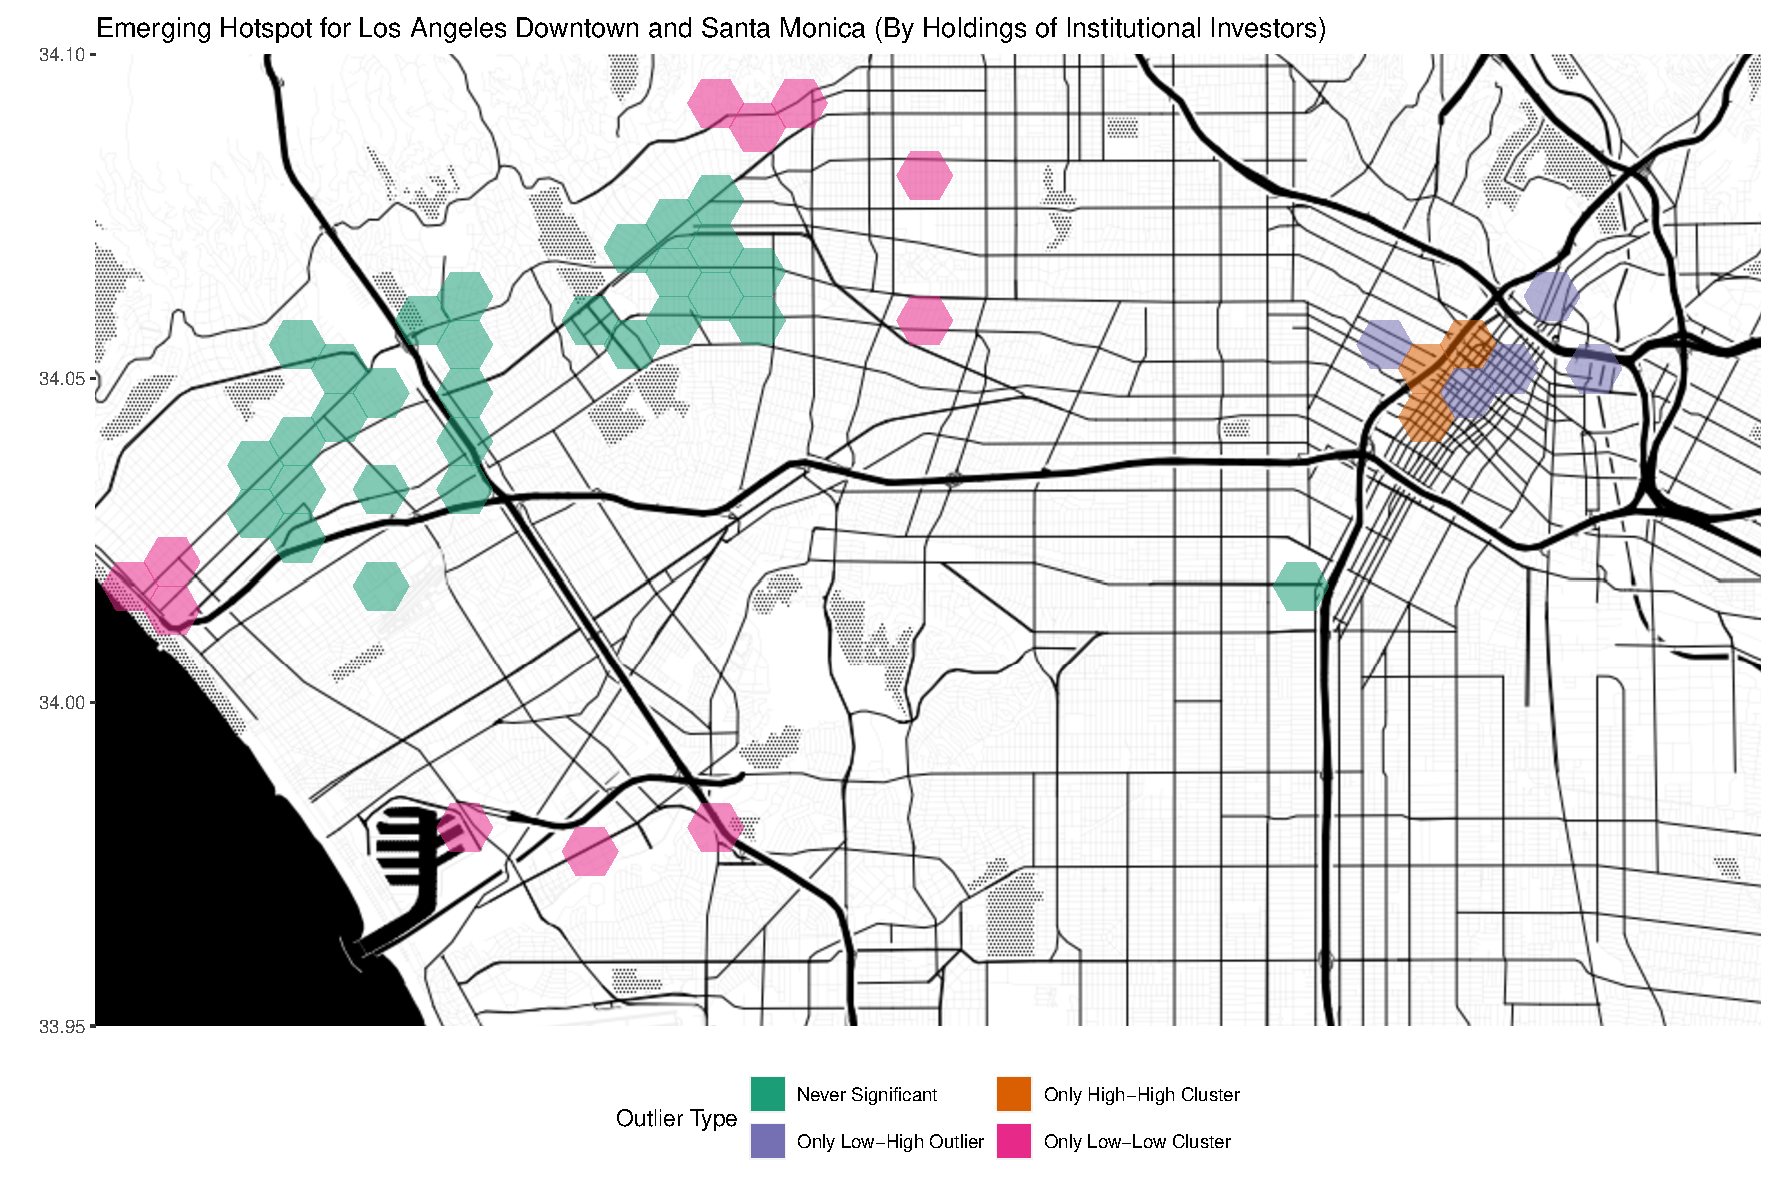
\includegraphics[width=1\linewidth]{Figures/ChapterIV/LA_Money_LO_Downtown}
	\caption[Downtown Los Angeles and Santa Monica Local Outlier Analysis - Funds Under Management 2013-2018]{Downtown Los Angeles and Santa Monica local outlier analysis - funds under management}
	\label{fig:LAlocaloutlier_Downtown}
\end{figure}

\section{New York City}

\subsection{Count Data}

Figure \ref{fig:NYCcounthotspot} displays the singular emerging hot spot cluster for the New York region.  Unsurprisingly, this hot spot covers the heart of the US financial universe: the Financial District and Midtown on Manhattan Island, and extending somewhat into the Bronx, Brooklyn and Hudson County, New Jersey.   Furthermore, the intensifying hotspot over Manhattan and the constant hot spot to the south of it is evidence in the shift northwards towards Midtown Manhattan due to the desire to be near the intercontinental exchange - that is to say where transatlantic fiber optic cables come to shore in North America.\todo{citation}     

Providing more detailed spatial resolution on high-high hot spots, Figure \ref{fig:NYCcountlocaloutliercount} finds that most of the high-high hexes are located in Manhattan, and a few isolated hexes are located in Brooklyn, Bronx and Hudson Counties.  Notable by its absence, the highly residential Stuyvesant Town neighbourhood on the east side of Manhattan is largely devoid of institutional investors.      



\begin{figure}
	\centering
	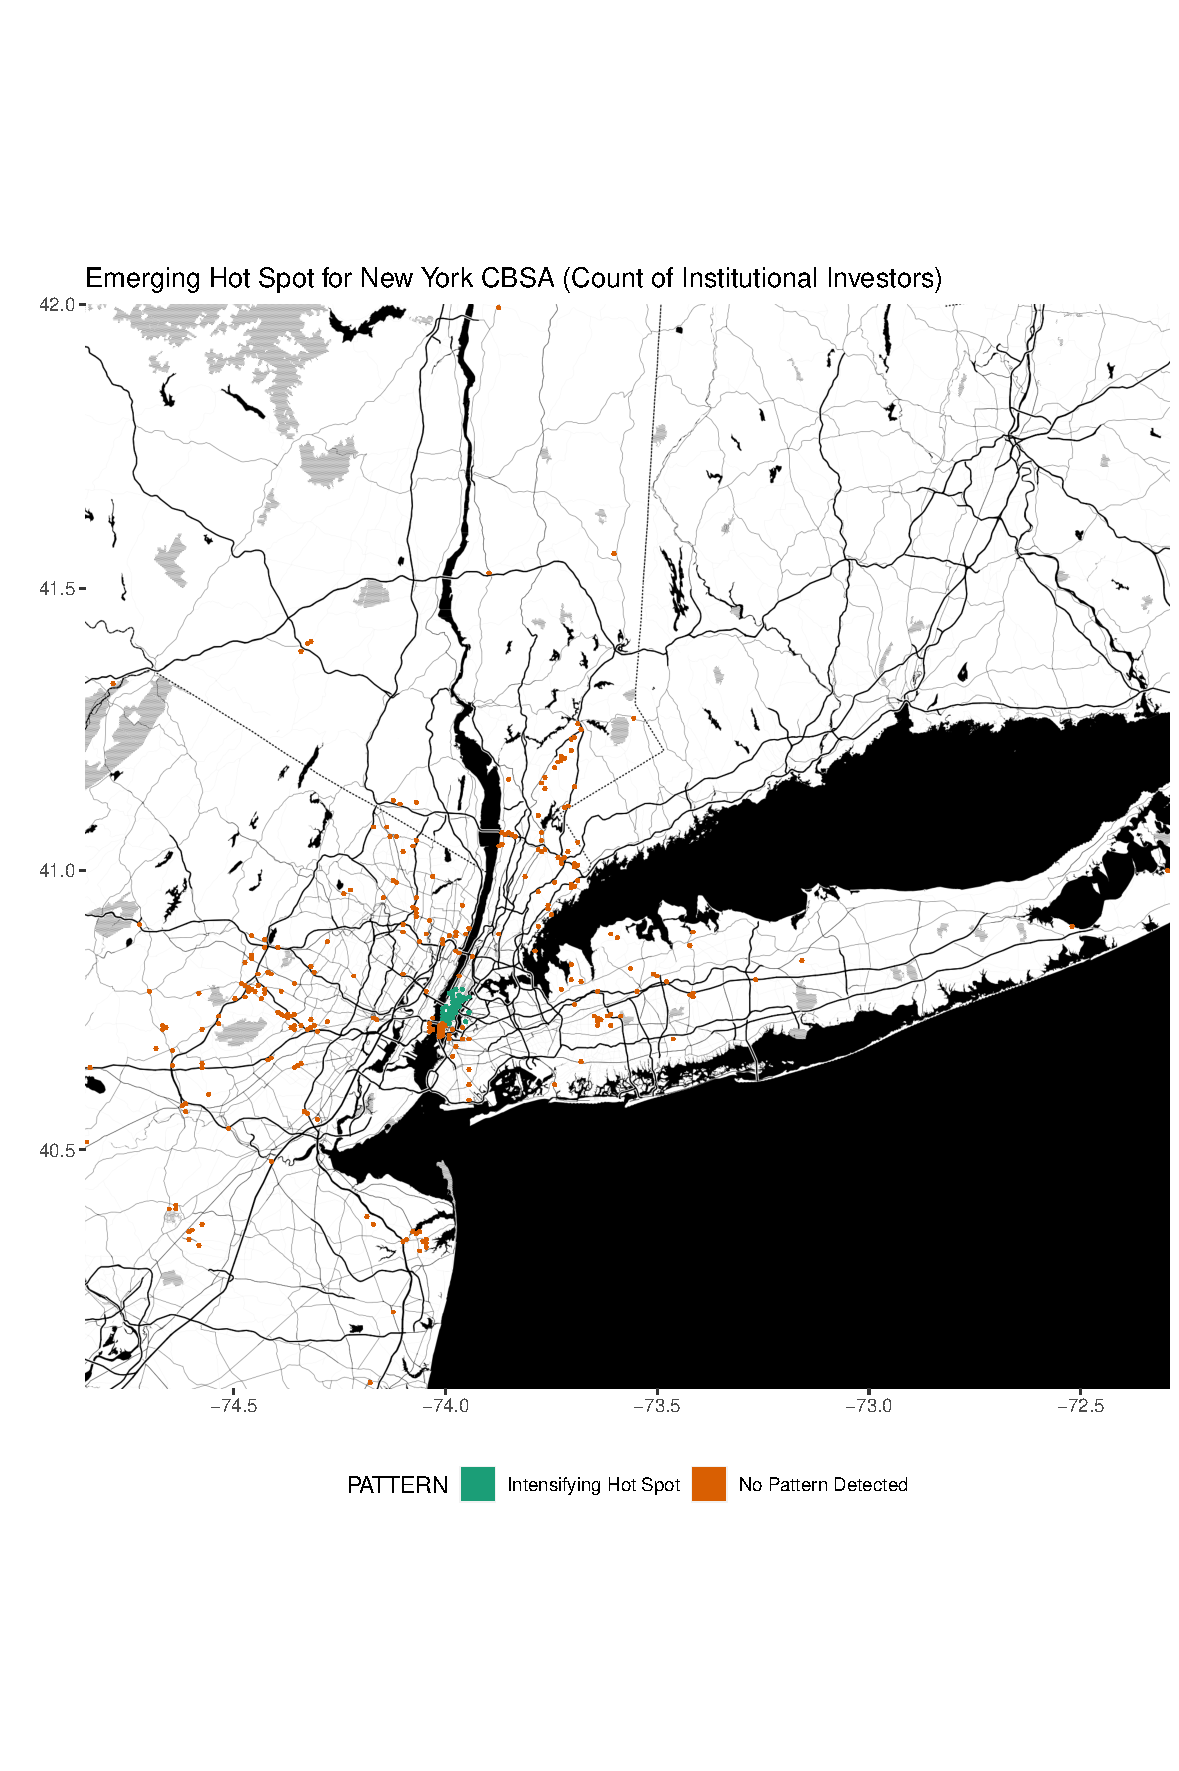
\includegraphics[width=1\linewidth]{Figures/ChapterIV/NY_Count_EH}
	\caption[Hot Spot Analysis of Number of Firms in New York CBSA 1999-2018]{Hot spot analysis of number of firms in New York for the time period March 1999 to December 2018}
	\label{fig:NYCcounthotspot}
\end{figure}


\begin{figure}
	\centering
	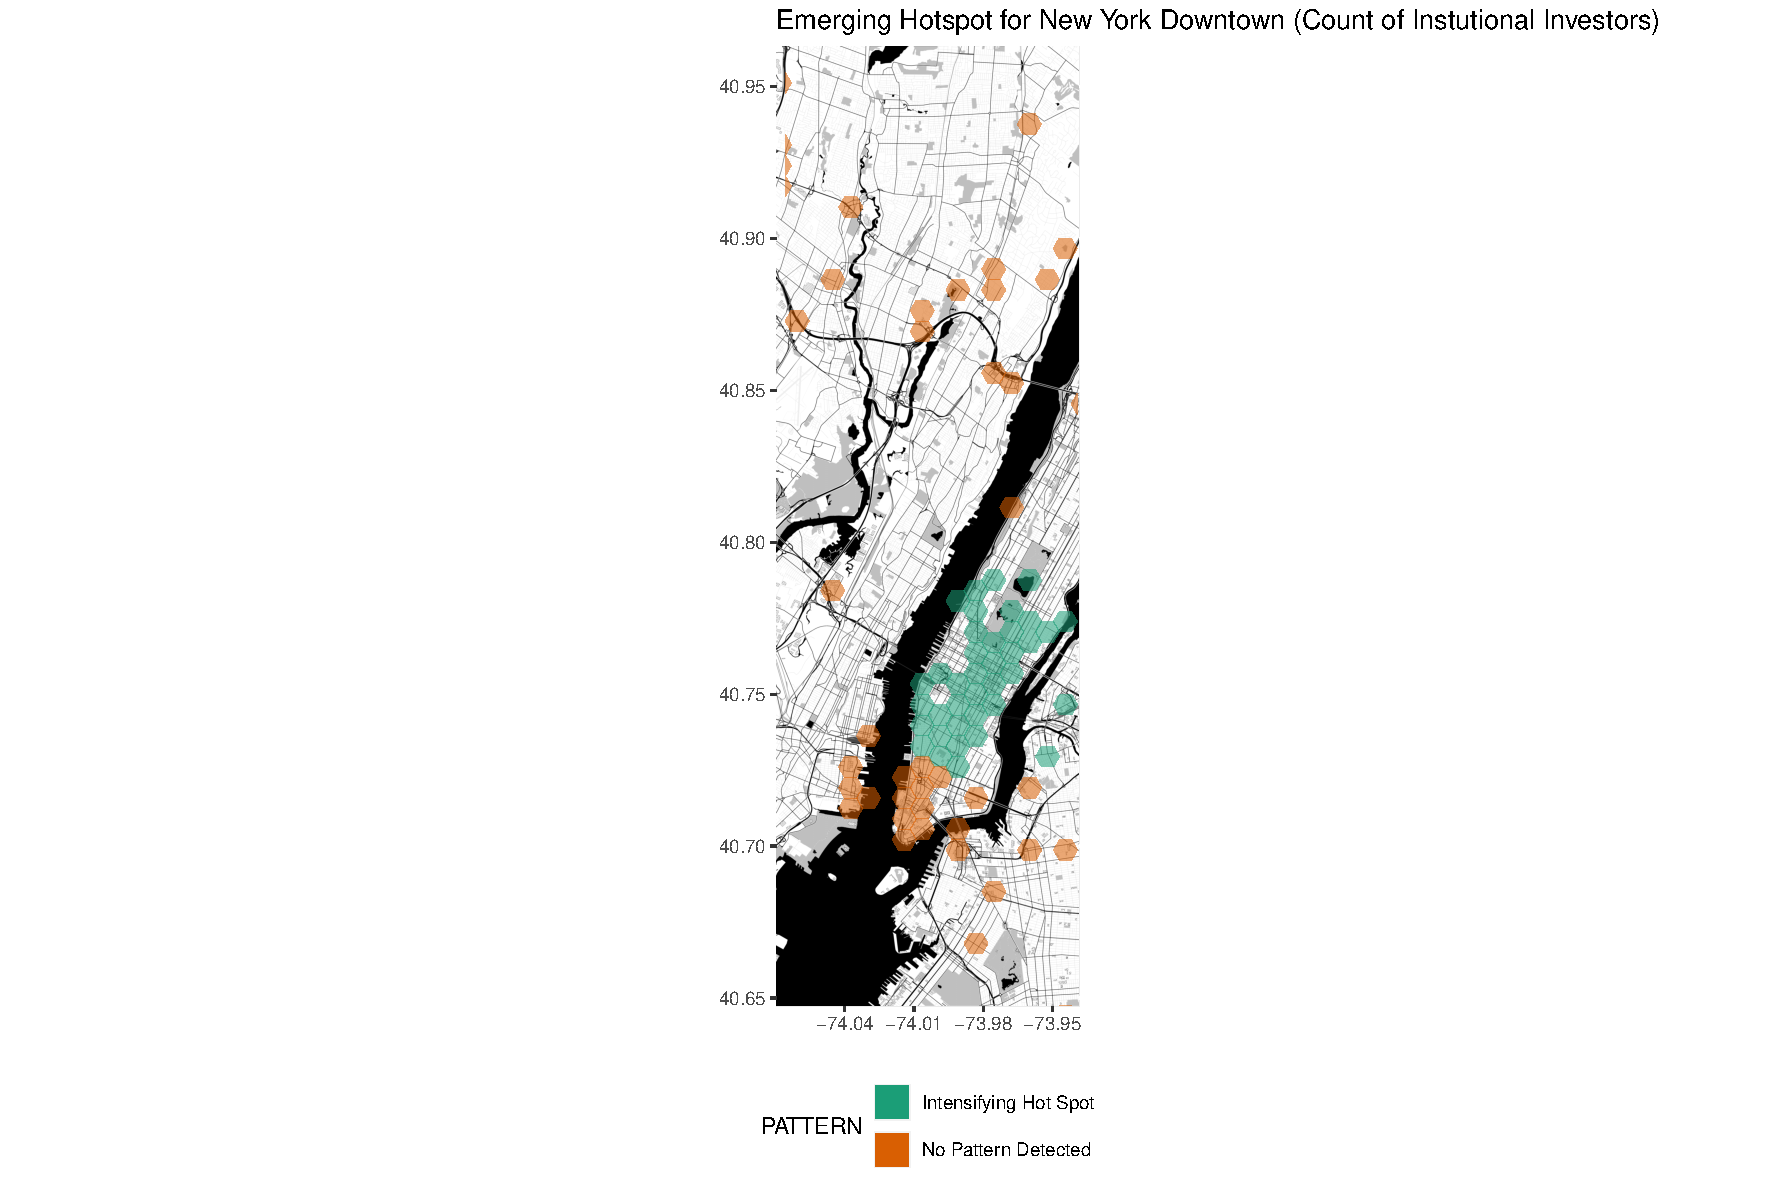
\includegraphics[width=1\linewidth]{Figures/ChapterIV/NY_Count_EH_Downtown}
	\caption[Hot Spot Analysis of Number of Firms in Downtown New York 1999-2018]{Hot spot analysis of number of firms in downtown New York for the time period March 1999 to December 2018}
	\label{fig:NYCcounthotspot_Downtown}
\end{figure}

\begin{figure}
	\centering
	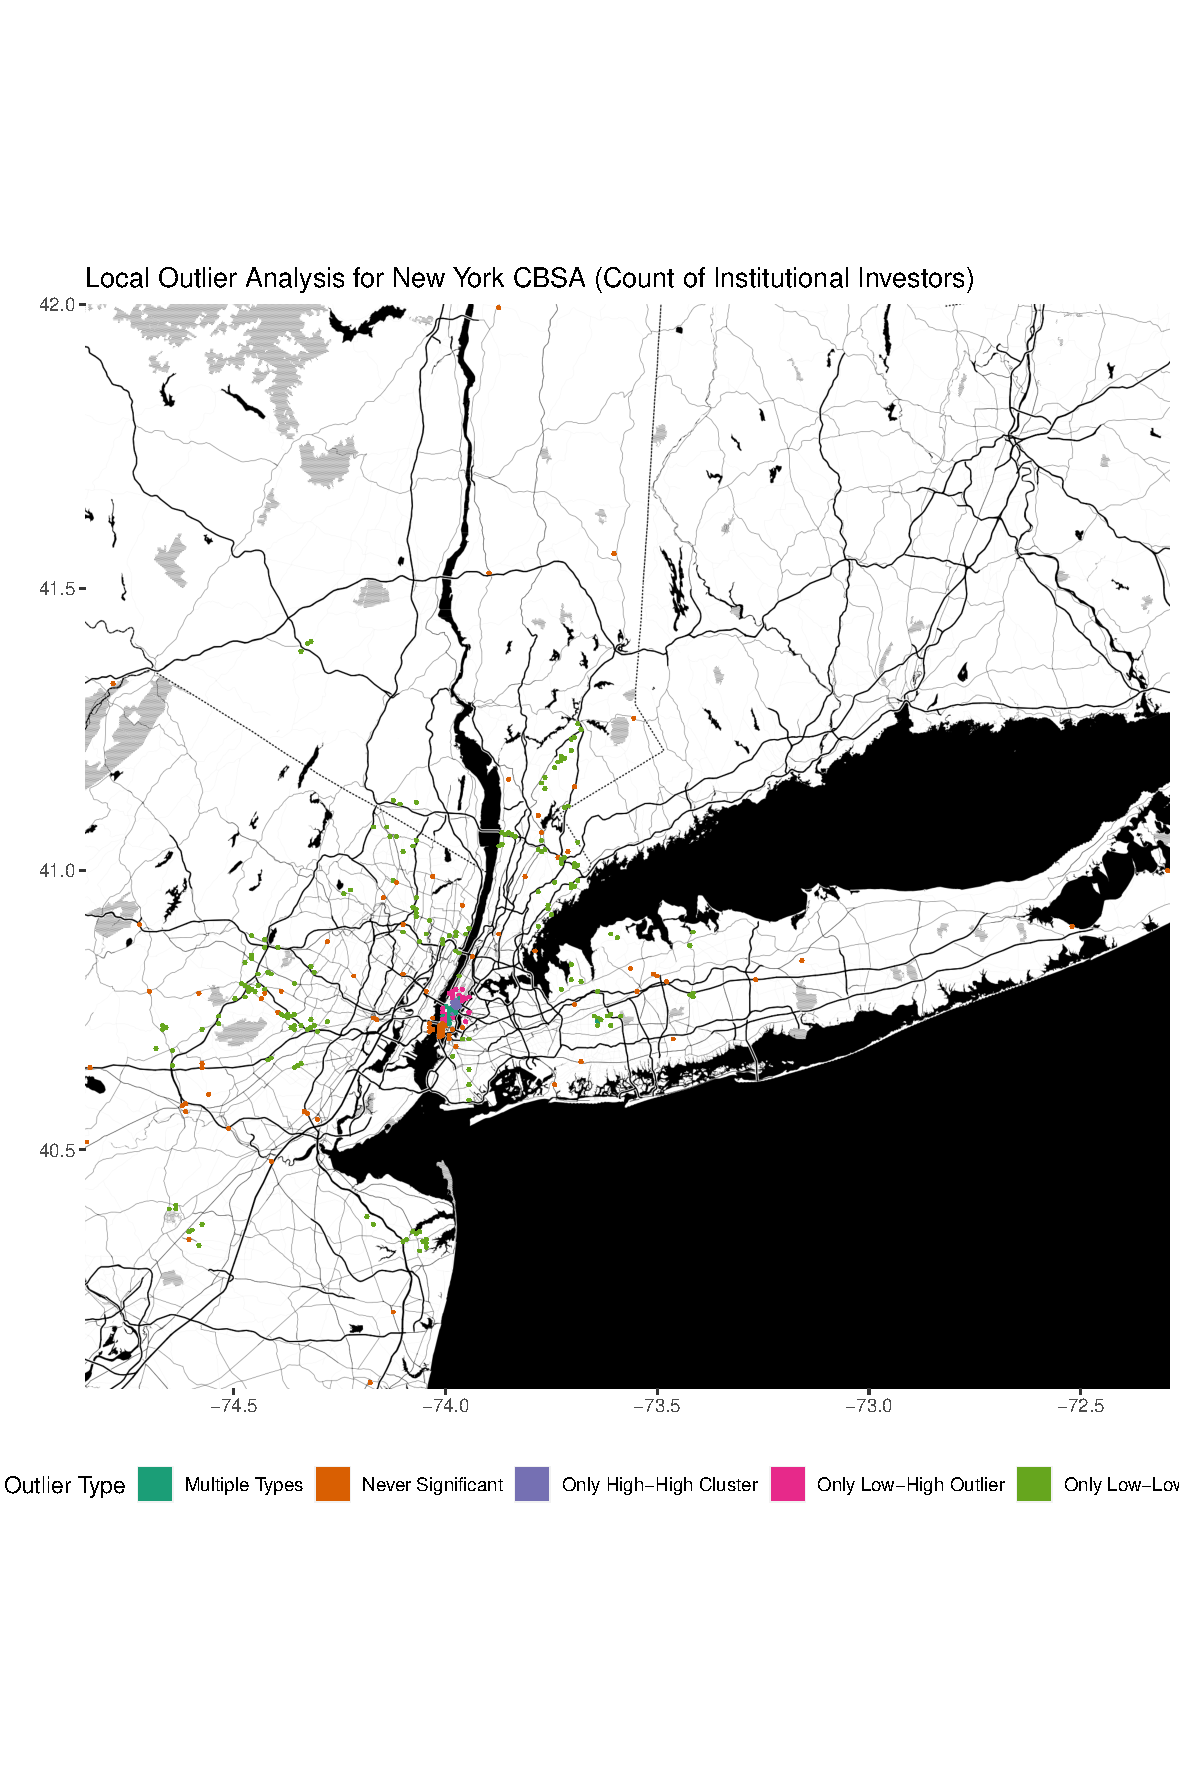
\includegraphics[width=1\linewidth]{Figures/ChapterIV/NY_Count_LO}
	\caption[New York CBSA Local Outlier Analysis - Count of Institutional Investors 1999-2018]{New York local outlier analysis - count of institutional investors}
	\label{fig:NYCcountlocaloutliercount}
\end{figure}	

\begin{figure}
	\centering
	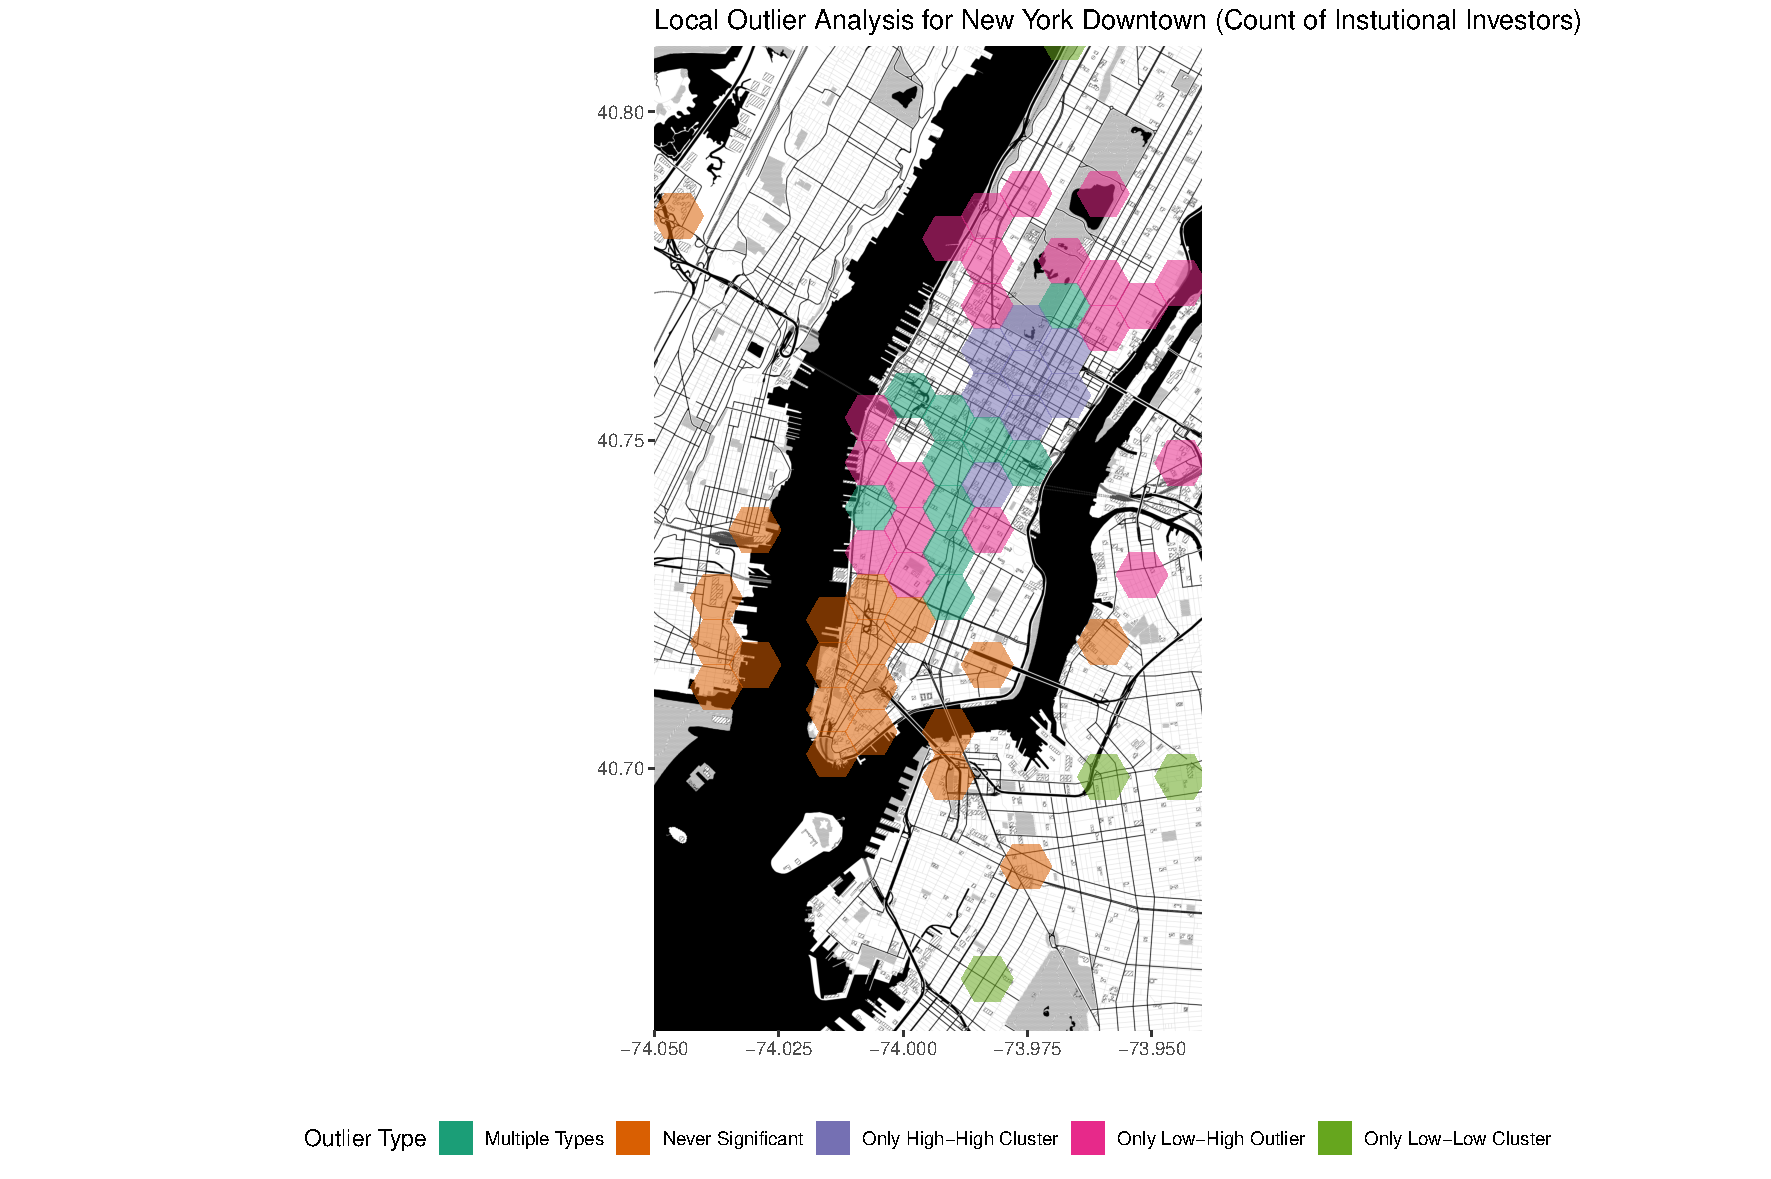
\includegraphics[width=1\linewidth]{Figures/ChapterIV/NY_Count_LO_Downtown}
	\caption[Downtown New York Local Outlier Analysis - Count of Institutional Investors 1999-2018]{Downtown New York local outlier analysis - count of institutional investors}
	\label{fig:NYCcountlocaloutliercount_Downtown}
\end{figure}
\subsection{Funds Under Management}

Once again, the use of funds under management as the unit of measure for emerging hot spot analysis shows a more restrictive hot spot. In fact, Figure \ref{fig:NYCmoneyhotspot} is simply a more restrictive version of Figure \ref{fig:NYCcounthotspot}.  The same can be said of Figure \ref{fig:NYClocaloutlier} treatment of local outlier analysis when compared to Figure \ref{fig:NYCcountlocaloutliercount}.  That being said, this more restrictive criteria removes most of the high-high clusters in Hudson County and Brooklyn County, suggesting once again that these investors located outside of the CBD have a smaller bankroll than the investors located in the CBD.   

\begin{figure}
	\centering
	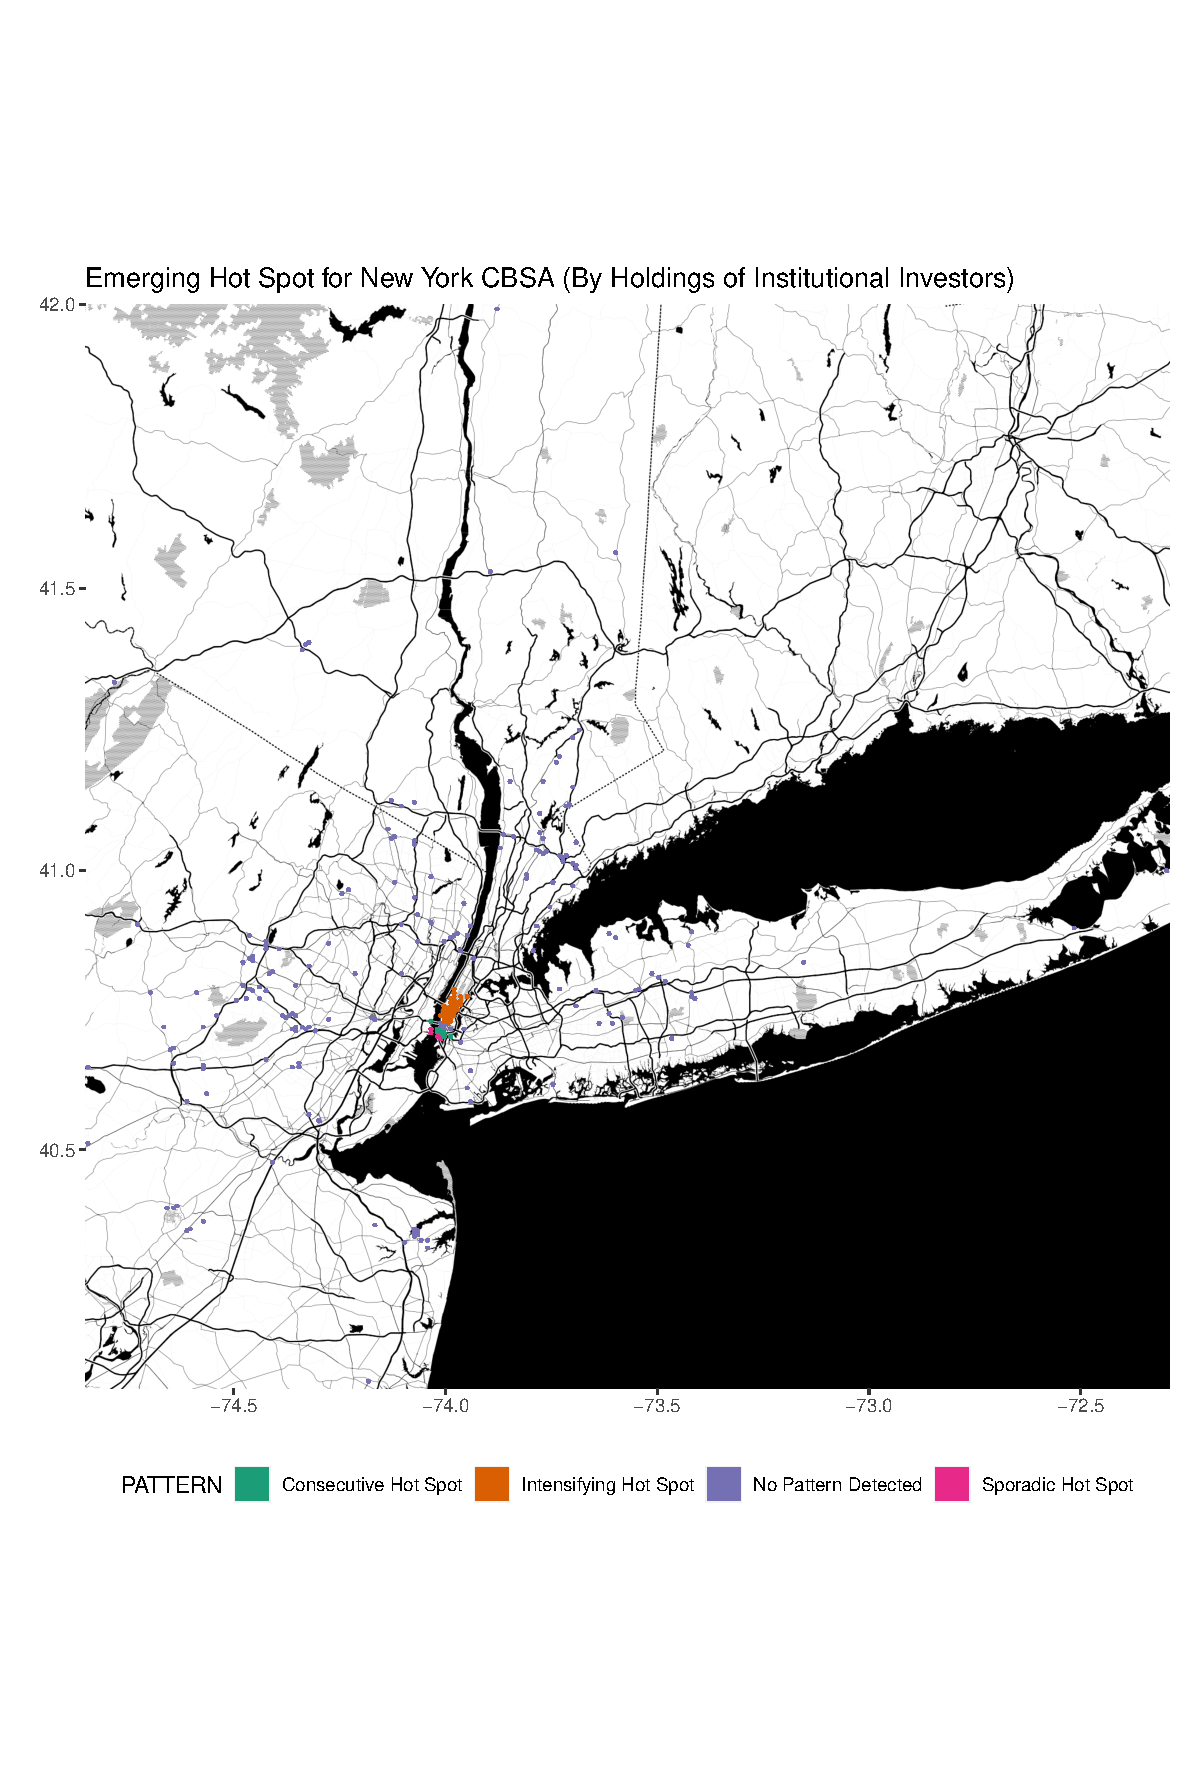
\includegraphics[width=1\linewidth]{Figures/ChapterIV/NY_Money_EH}
	\caption[Emerging Hot Spot Analysis of Funds Under Management for New York CBSA 2013-2018]{Emerging hot spot analysis of funds under management for New York for period June 2013 to December 2018}
	\label{fig:NYCmoneyhotspot}
\end{figure}

\begin{figure}
	\centering
	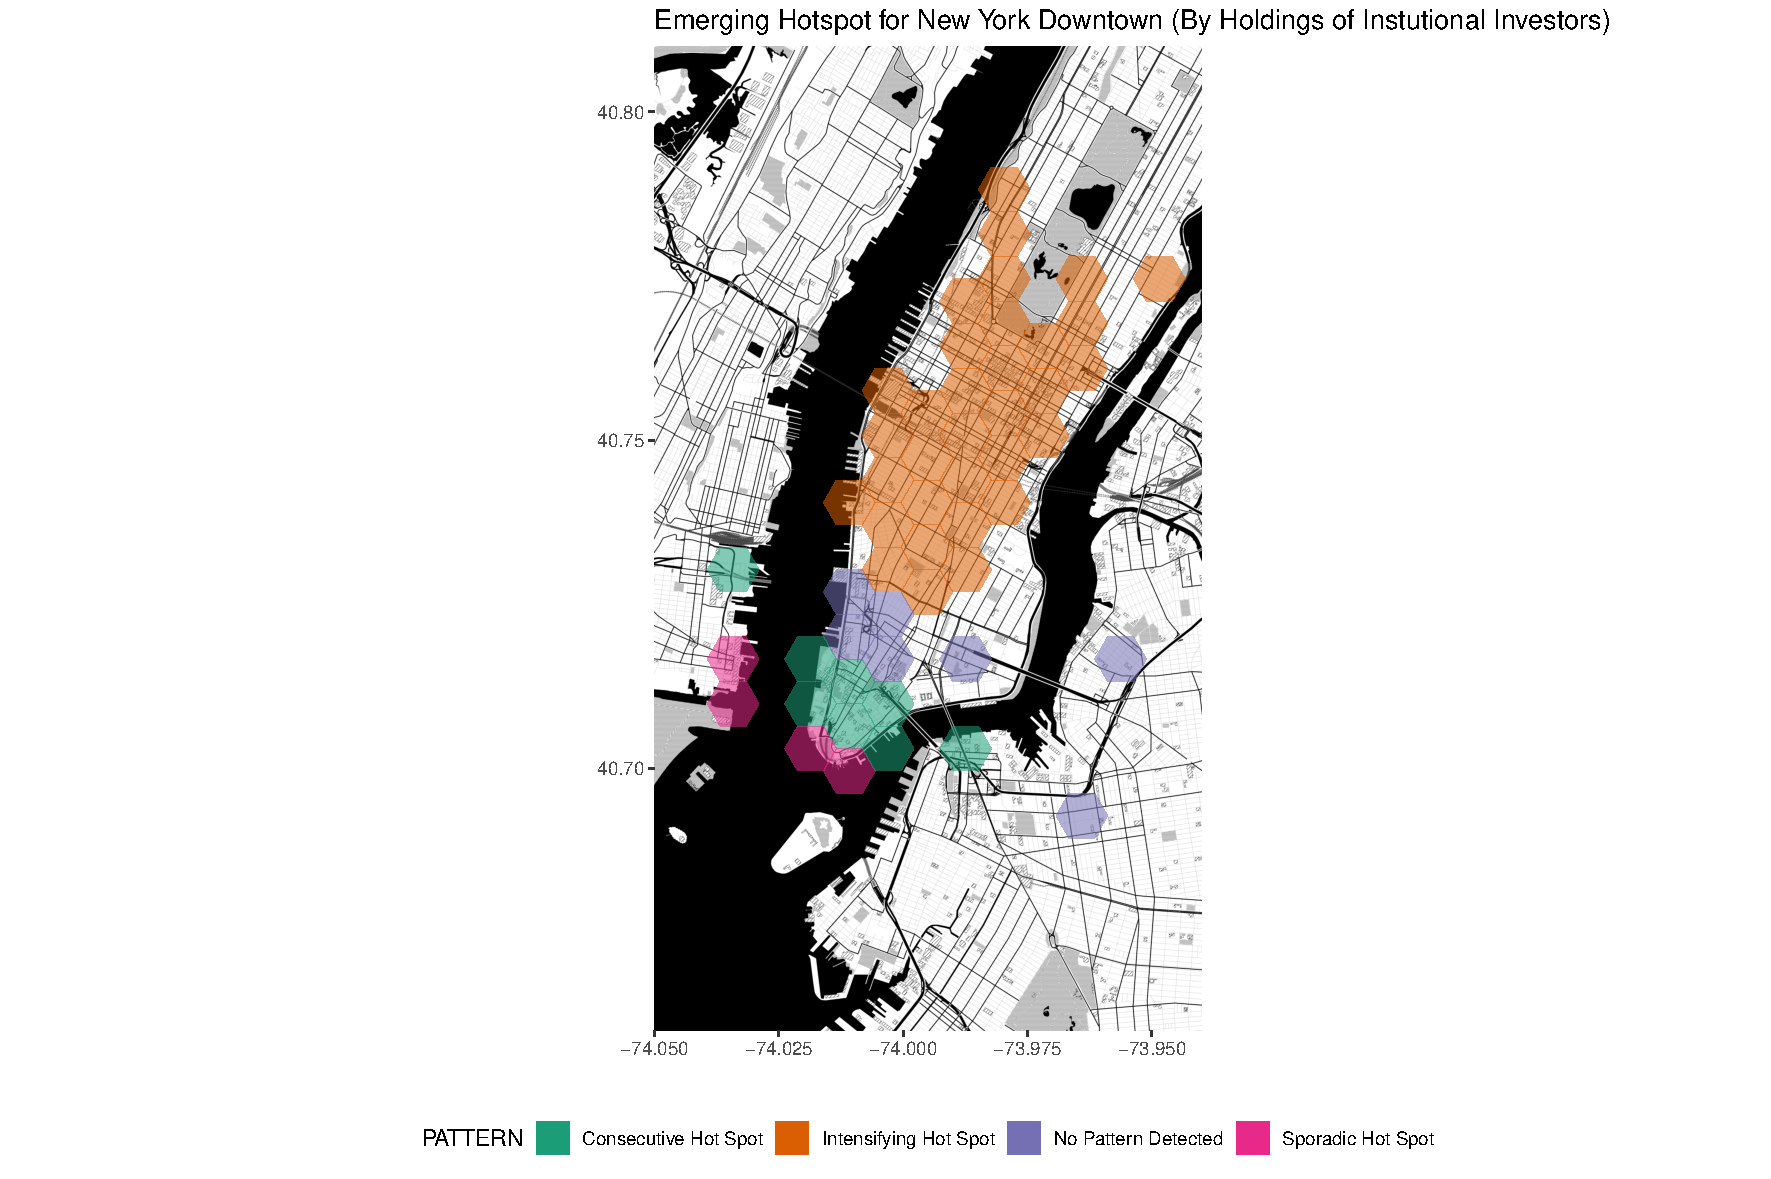
\includegraphics[width=1\linewidth]{Figures/ChapterIV/NY_Money_EH_Downtown}
	\caption[Emerging Hot Spot Analysis of Funds Under Management for Downtown New York 2013-2018]{Emerging hot spot analysis of funds under management for downtown New York for period June 2013 to December 2018}
	\label{fig:NYCmoneyhotspot_Downtown}
\end{figure}


\begin{figure}
	\centering
	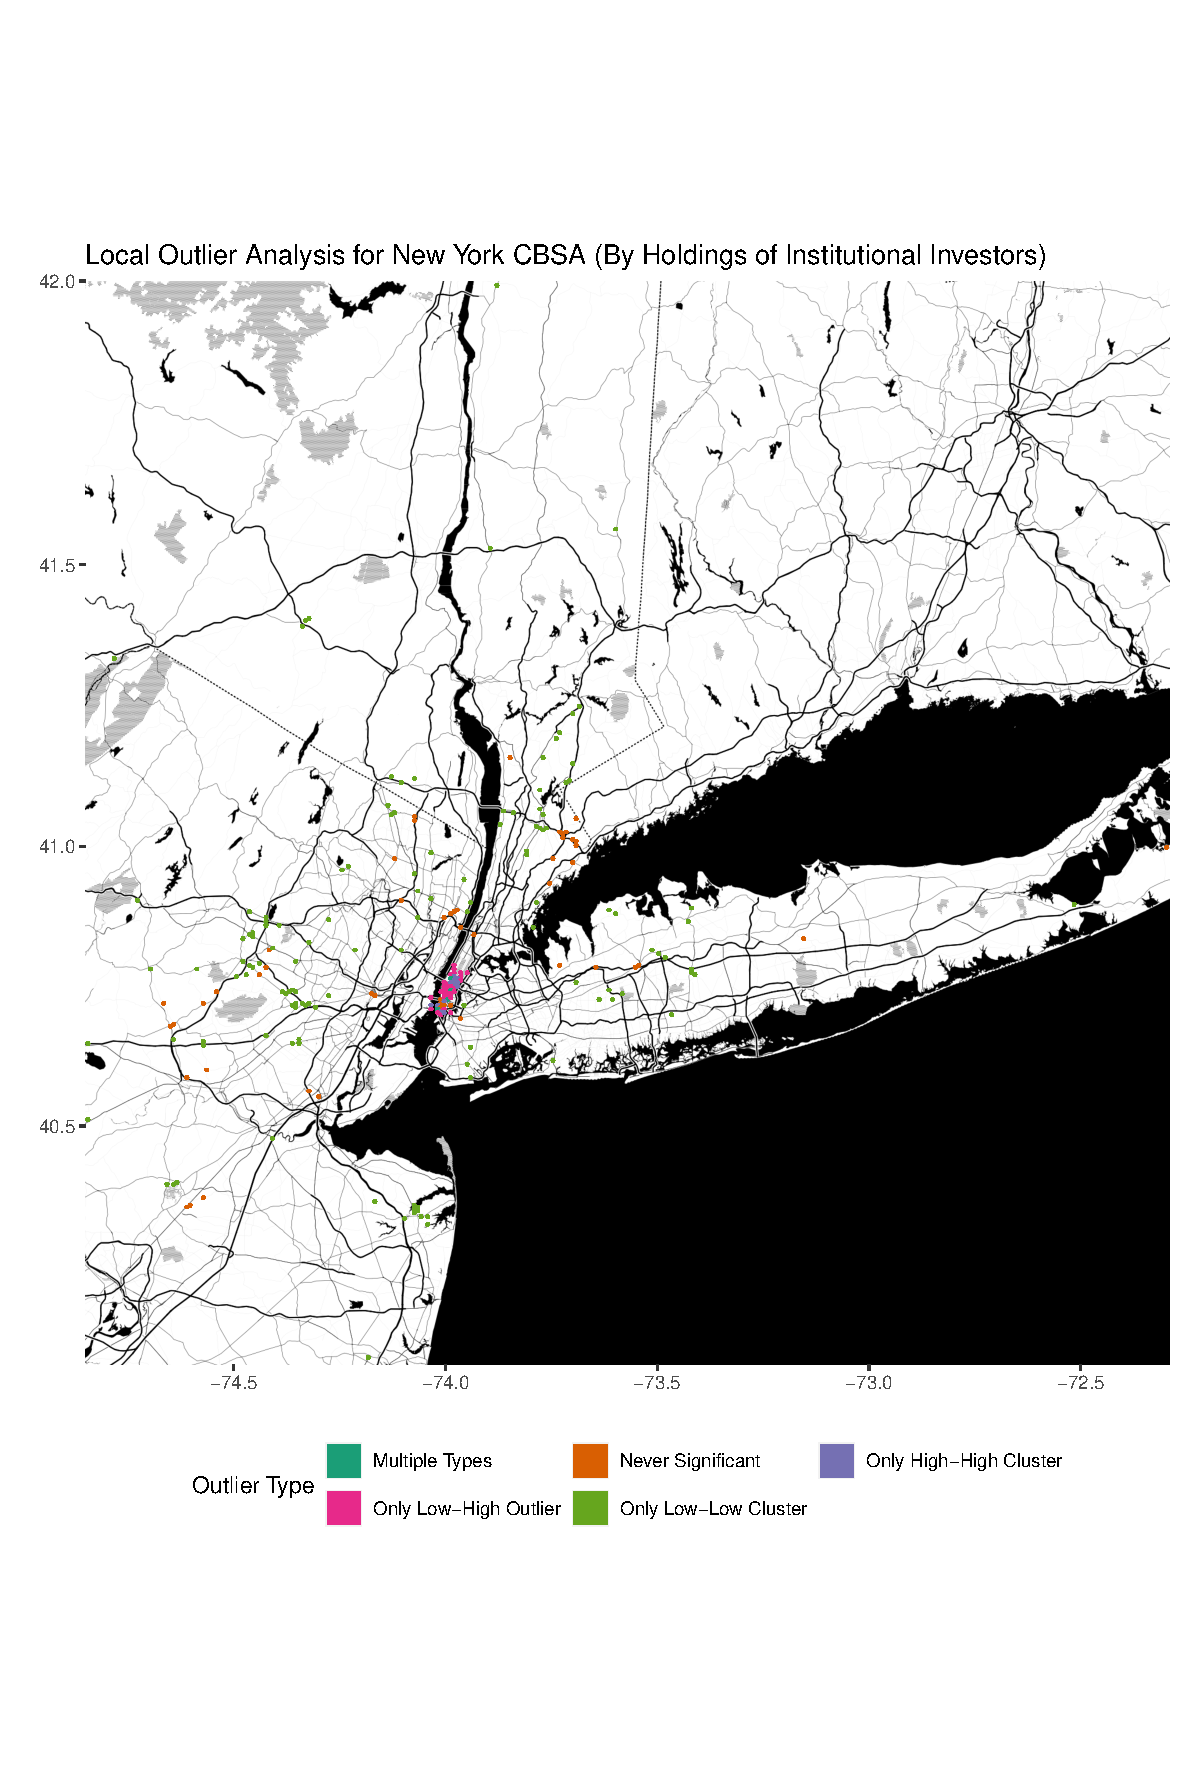
\includegraphics[width=1\linewidth]{Figures/ChapterIV/NY_Money_LO}
	\caption[New York CBSA Local Outlier Analysis - Funds Under Management 2013-2018]{New York local outlier analysis - funds under management}
	\label{fig:NYClocaloutlier}
\end{figure}

\begin{figure}
	\centering
	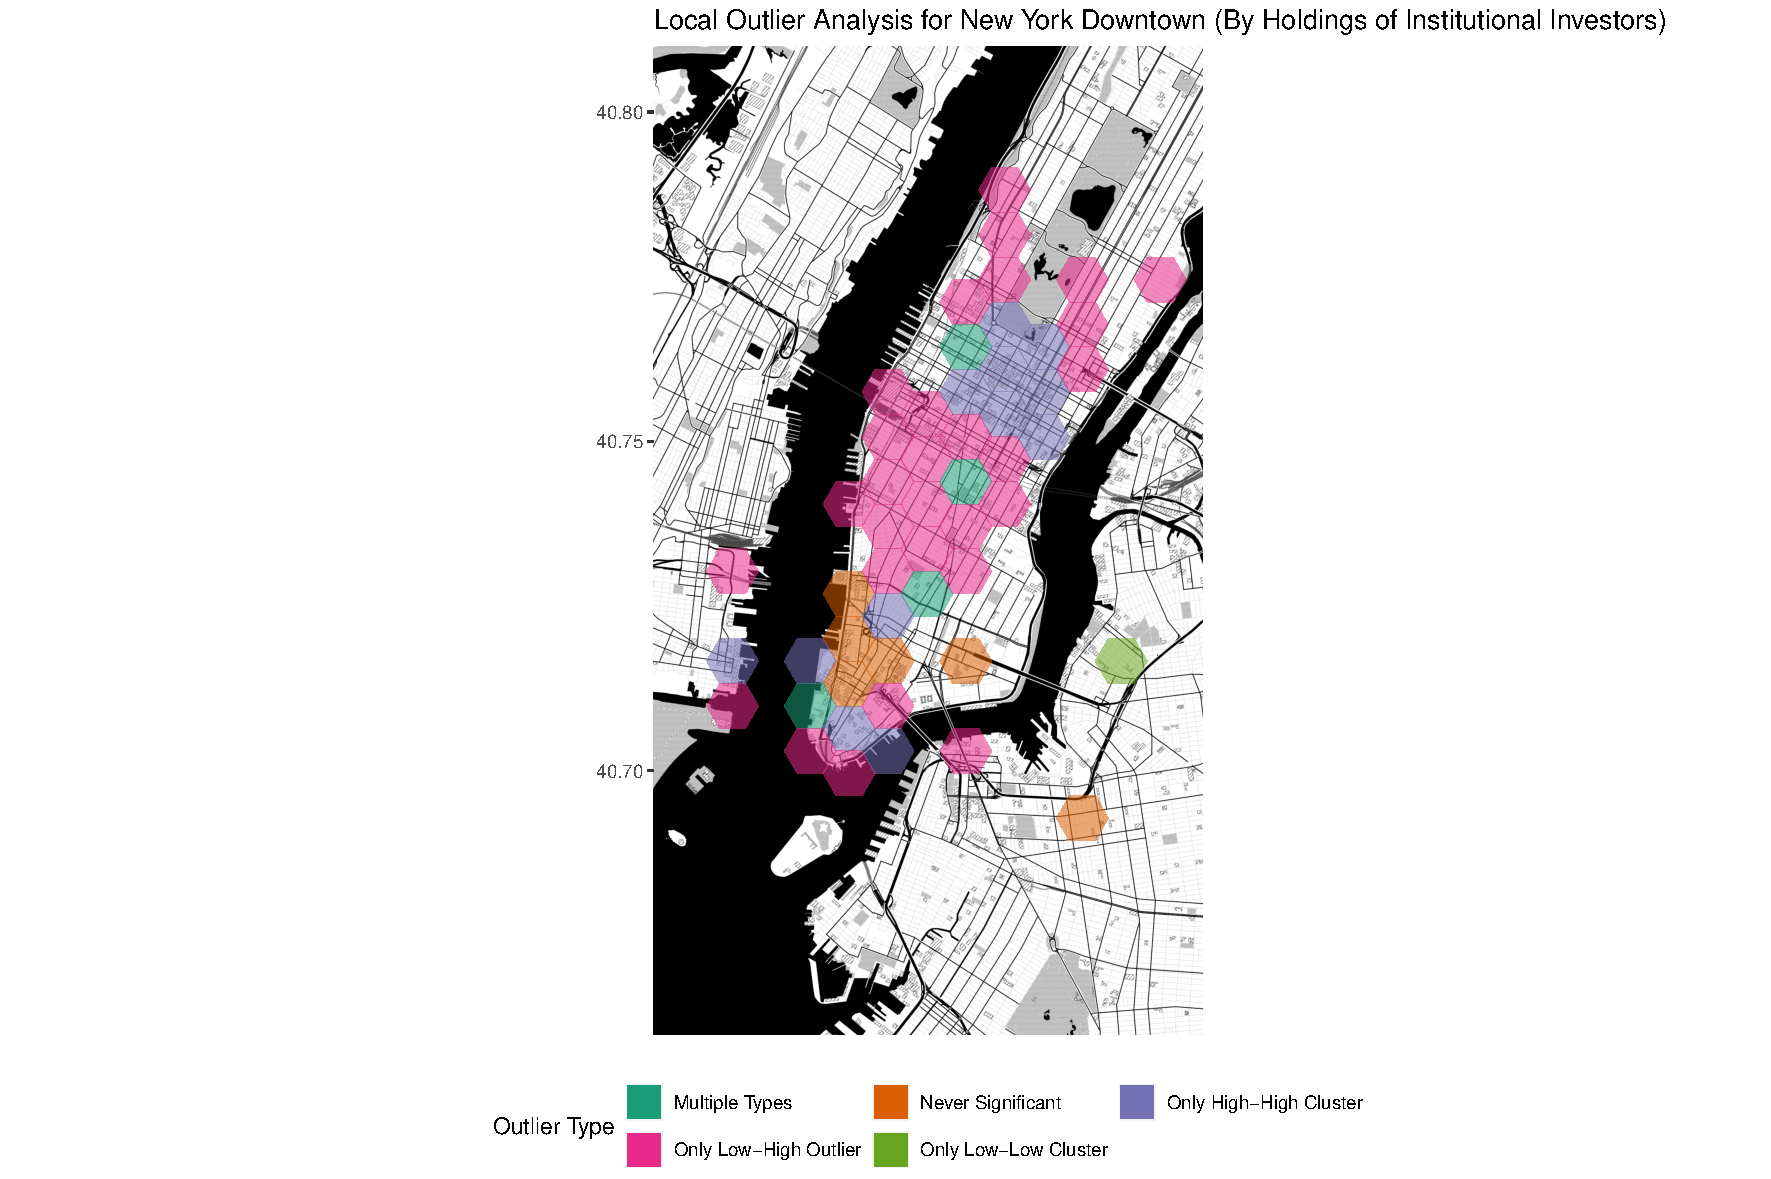
\includegraphics[width=1\linewidth]{Figures/ChapterIV/NY_Money_LO_Downtown}
	\caption[Downtown New York Local Outlier Analysis - Funds Under Management 2013-2018]{Downtown New York local outlier analysis - funds under management}
	\label{fig:NYClocaloutlier_Downtown}
\end{figure}


\section{San Francisco}


\subsection{Count Data}

Figure \ref{fig:SFcounthotspot} displays five hot spots: an emerging hot spot in San Francisco's central business district, San Mateo, a small emerging centre north of the Golden Gate Bridge along with consecutive hot spots in Palo Alto and Walnut Creek.   

\begin{figure}
	\centering
	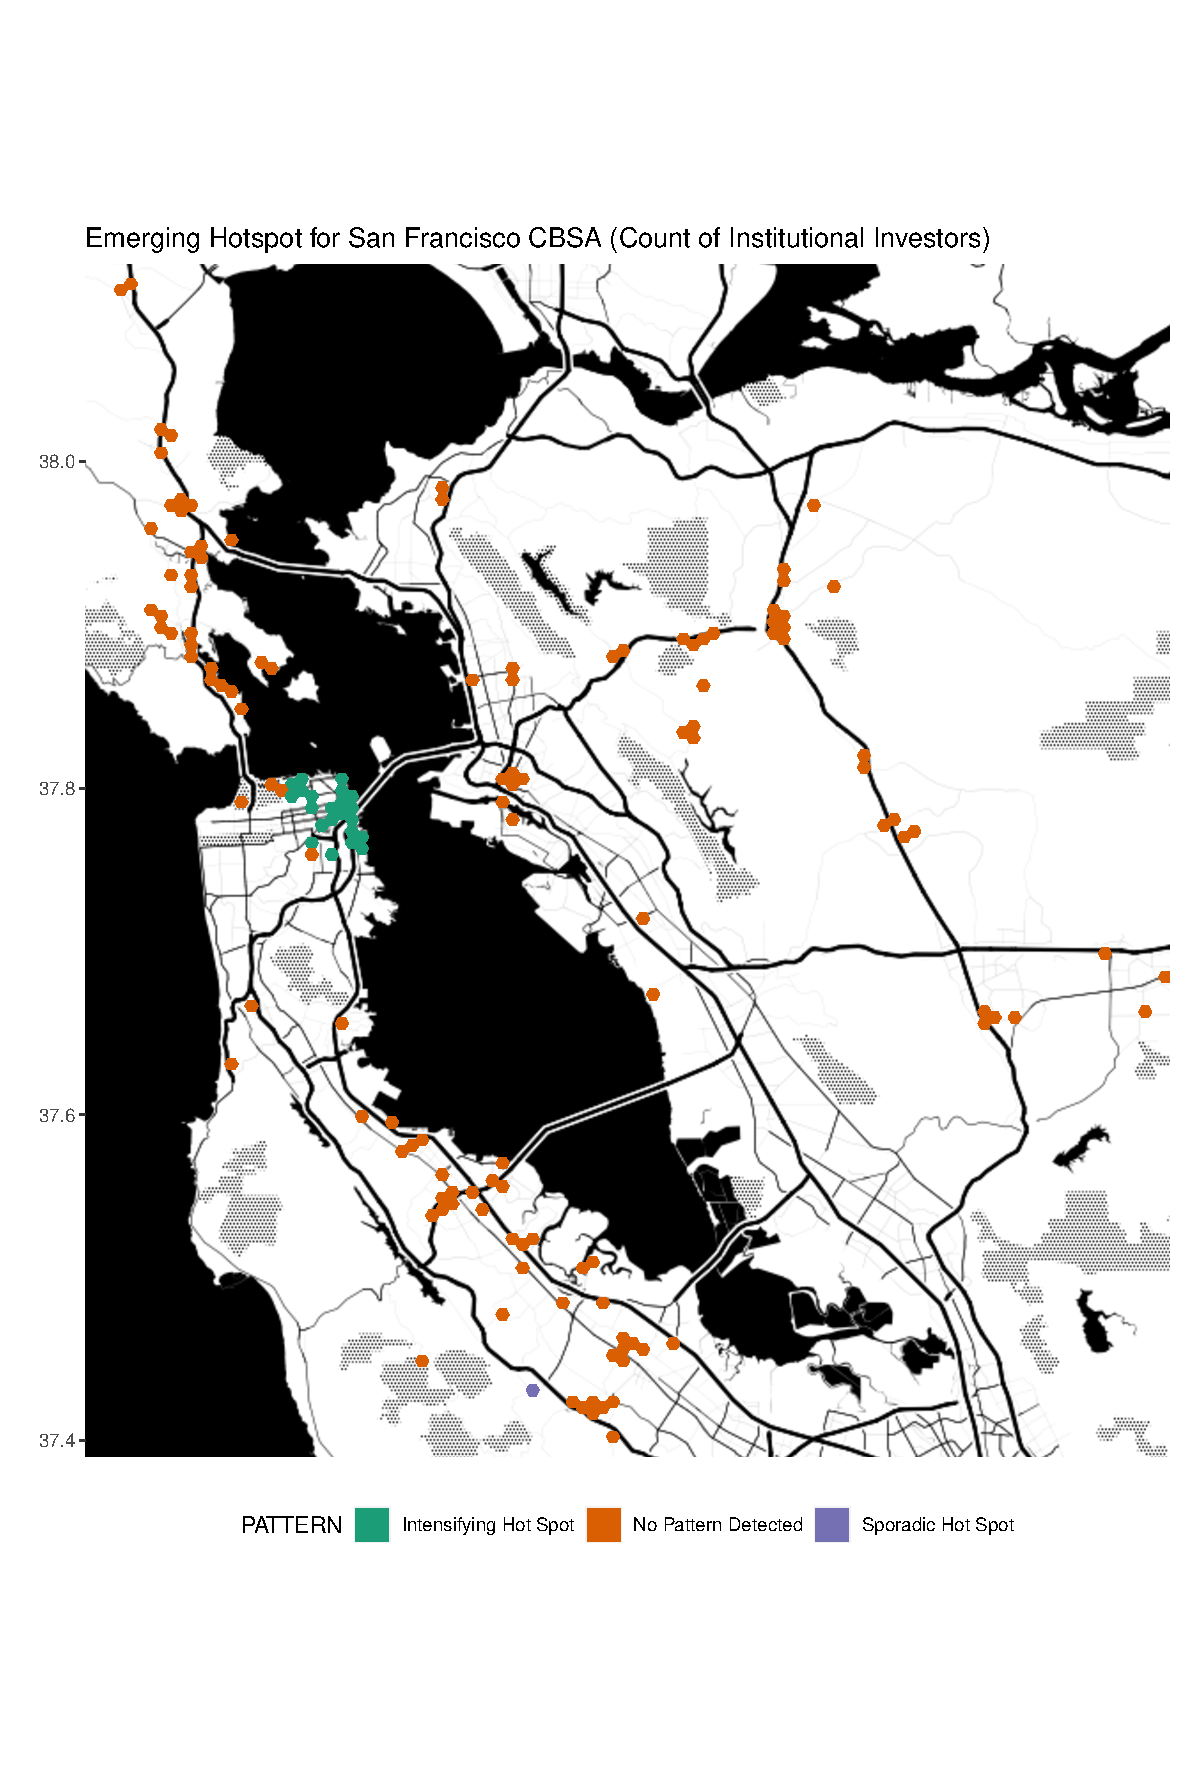
\includegraphics[width=1\linewidth]{Figures/ChapterIV/SF_Count_EH}
	\caption[Hot Spot Analysis of Number of Firms in San Francisco CBSA 1999-2018]{Hot spot analysis of number of firms in San Francisco for the time period March 1999 to December 2018}
	\label{fig:SFcounthotspot}
\end{figure}

\begin{figure}
	\centering
	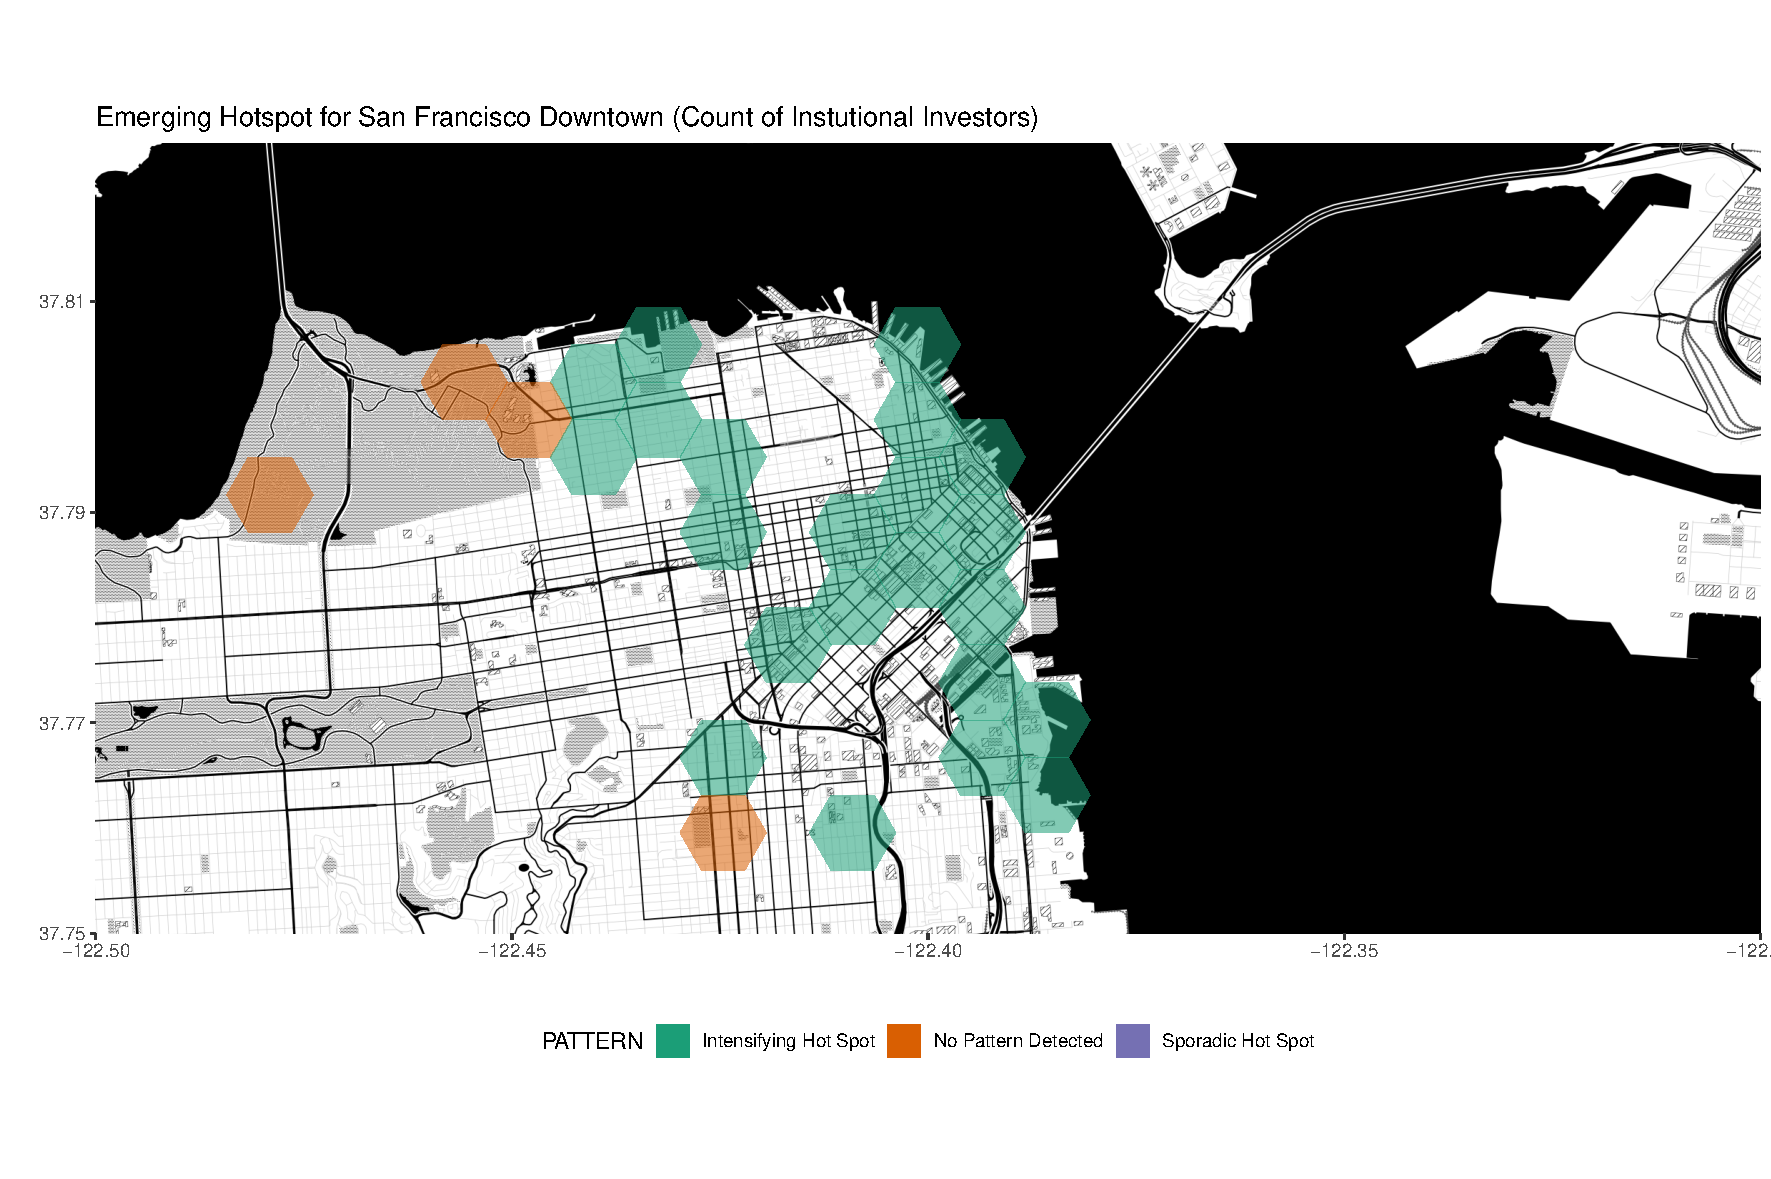
\includegraphics[width=1\linewidth]{Figures/ChapterIV/SF_Count_EH_Downtown}
	\caption[Hot Spot Analysis of Number of Firms in Downtown San Francisco 1999-2018]{Hot spot analysis of number of firms in downtown San Francisco for the time period March 1999 to December 2018}
	\label{fig:SFcounthotspot_Downtown}
\end{figure}

Figure \ref{fig:SFcountlocaloutliercount} displays the results of the local outlier analysis and finds the same five clusters.     

\begin{figure}
	\centering
	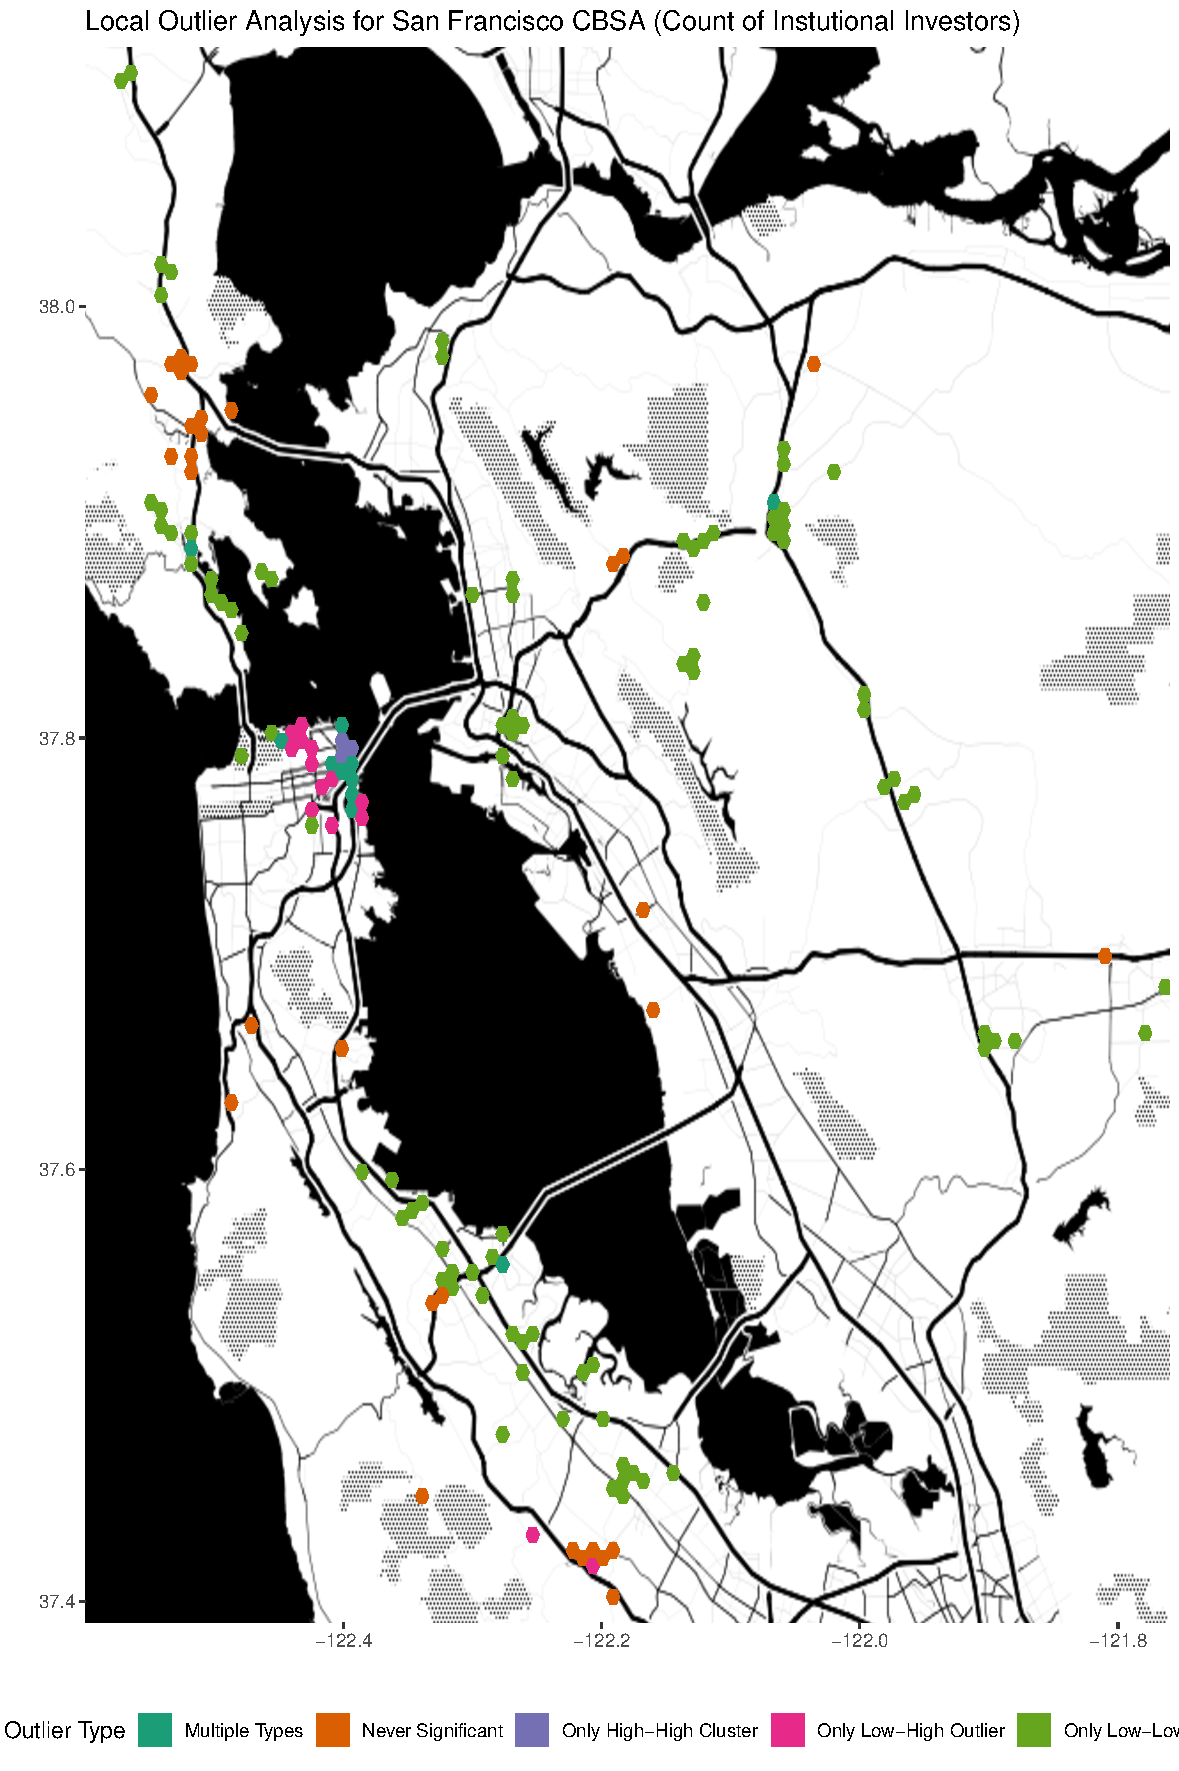
\includegraphics[width=1\linewidth]{Figures/ChapterIV/SF_Count_LO}
	\caption[San Francisco CBSA Local Outlier Analysis - Count of Institutional Investors 1999-2018]{San Francisco local outlier analysis - count of institutional investors}
	\label{fig:SFcountlocaloutliercount}
\end{figure}

\begin{figure}
	\centering
	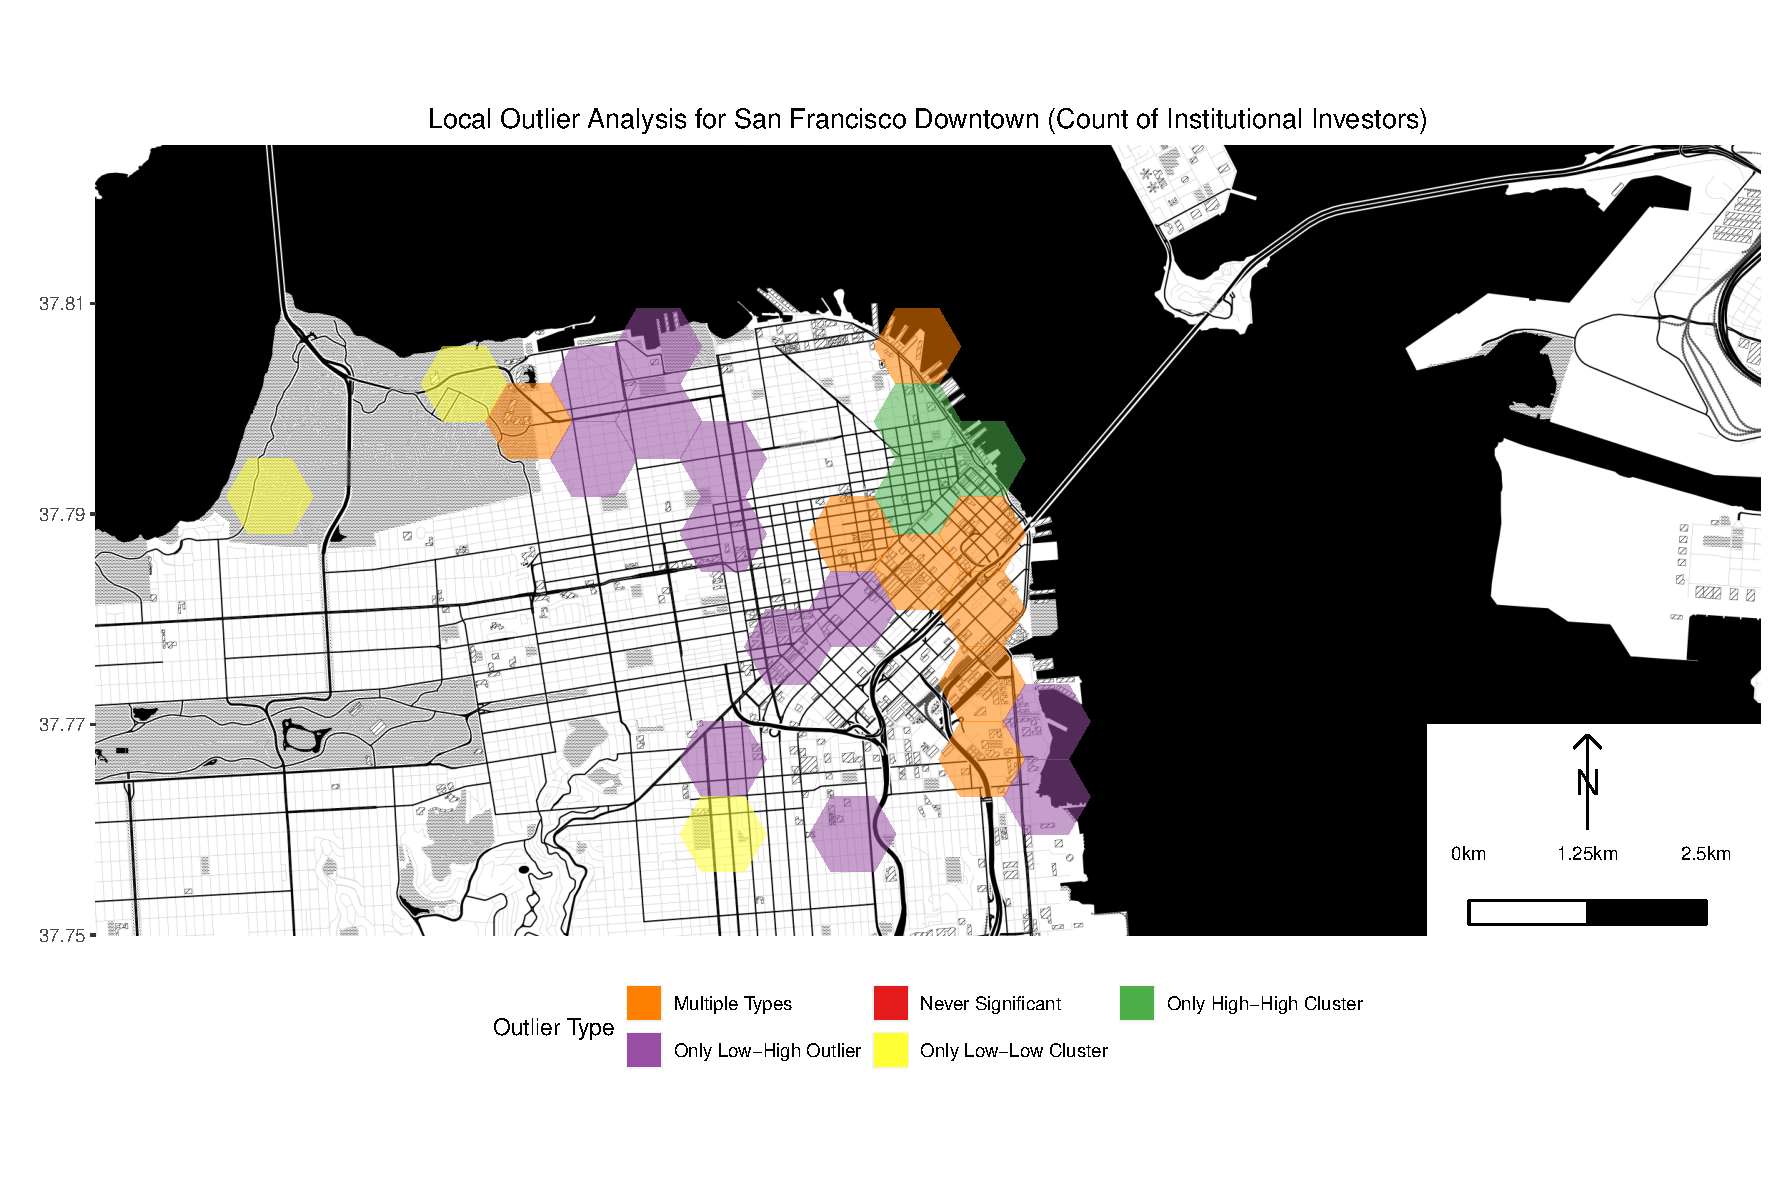
\includegraphics[width=1\linewidth]{Figures/ChapterIV/SF_Count_LO_Downtown}
	\caption[Downtown San Francisco Local Outlier Analysis - Count of Institutional Investors 1999-2018]{Downtown San Francisco local outlier analysis - count of institutional investors}
	\label{fig:SFcountlocaloutliercount_Downtown}
\end{figure}

\subsection{Funds Under Management}

In a continuing theme of having the funds under management Figures \ref{fig:SFnmoneyhotspot} and \ref{fig:SFlocaloutlier} show fewer hot spots than count data.  These hot spots are located in San Francisco's CBD and in San Mateo.  	

\begin{figure}
	\centering
	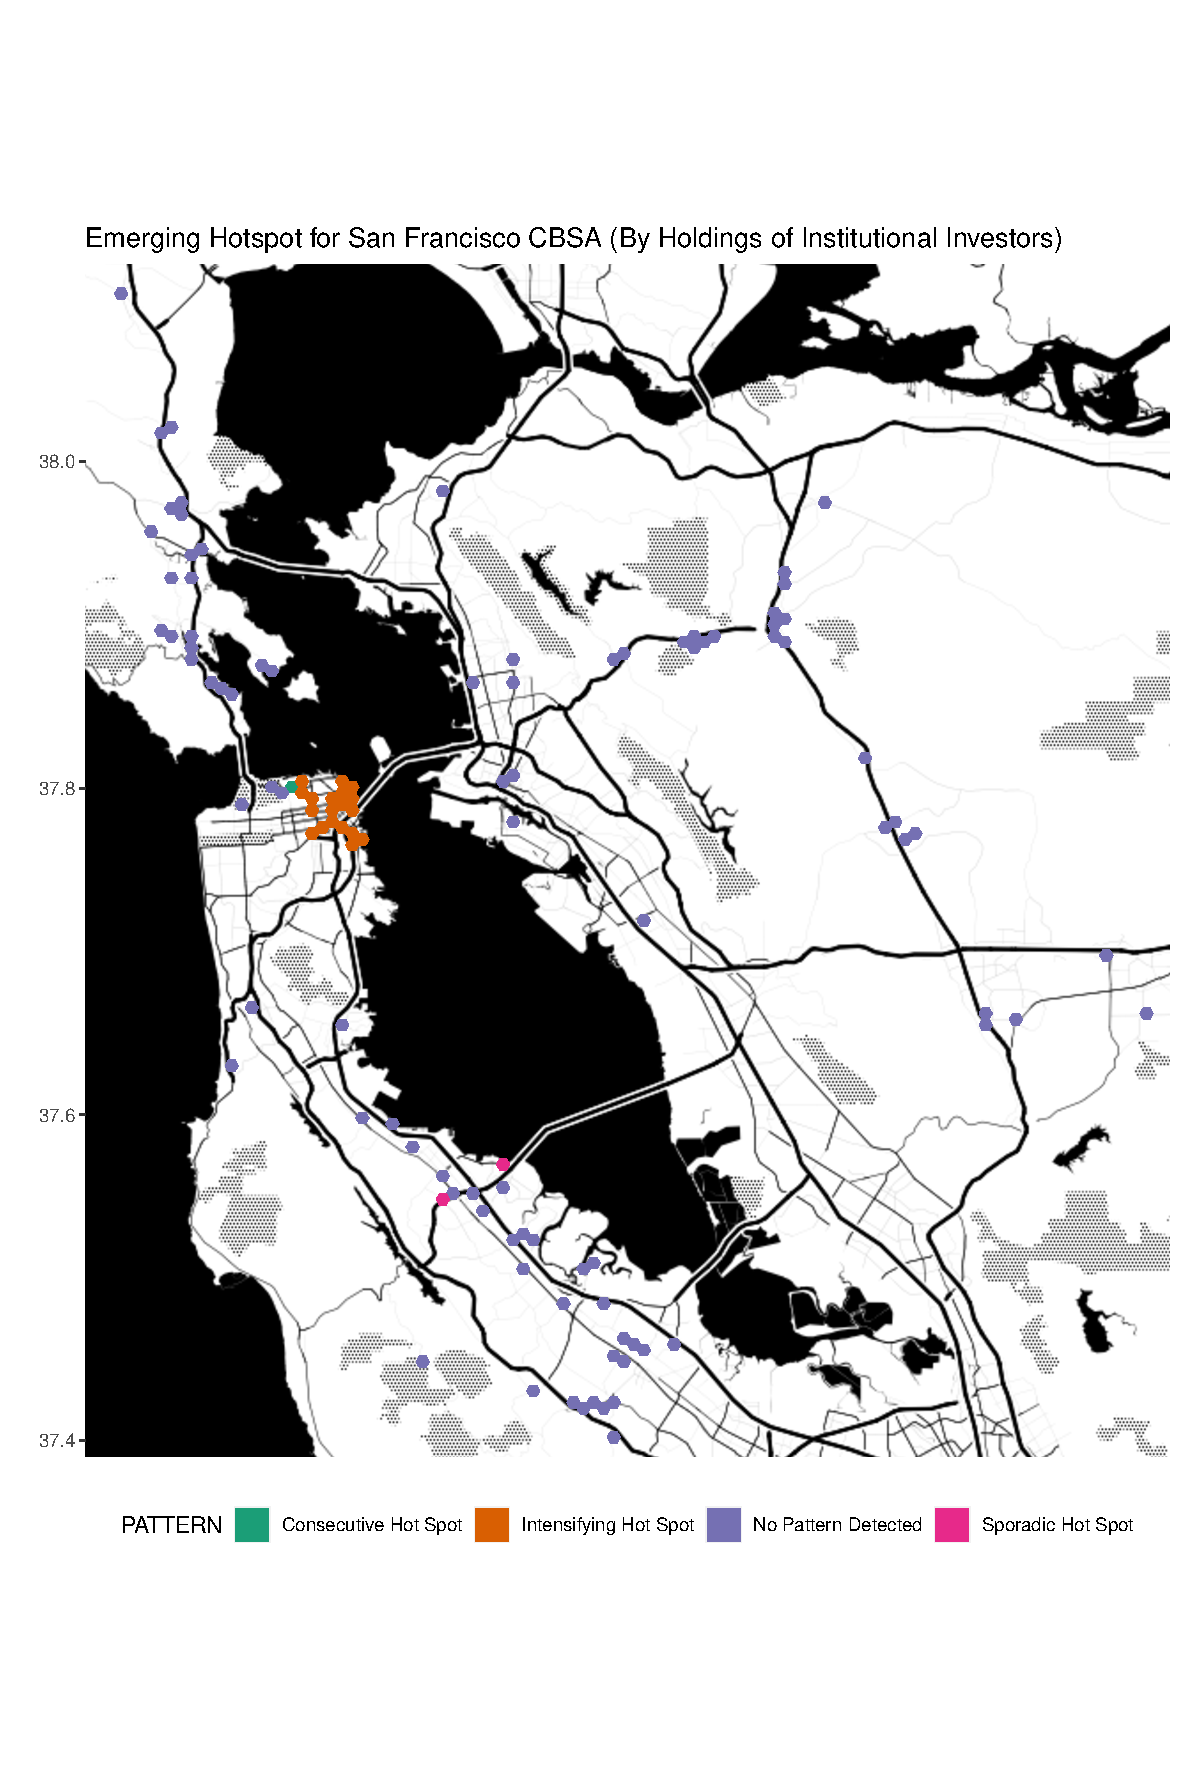
\includegraphics[width=1\linewidth]{Figures/ChapterIV/SF_Money_EH}
	\caption[Emerging Hot Spot Analysis of Funds Under Management for San Francisco CBSA 2013-2018]{Emerging hot spot analysis of funds under management for San Francisco for period June 2013 to December 2018}
	\label{fig:SFnmoneyhotspot}
\end{figure}

\begin{figure}
	\centering
	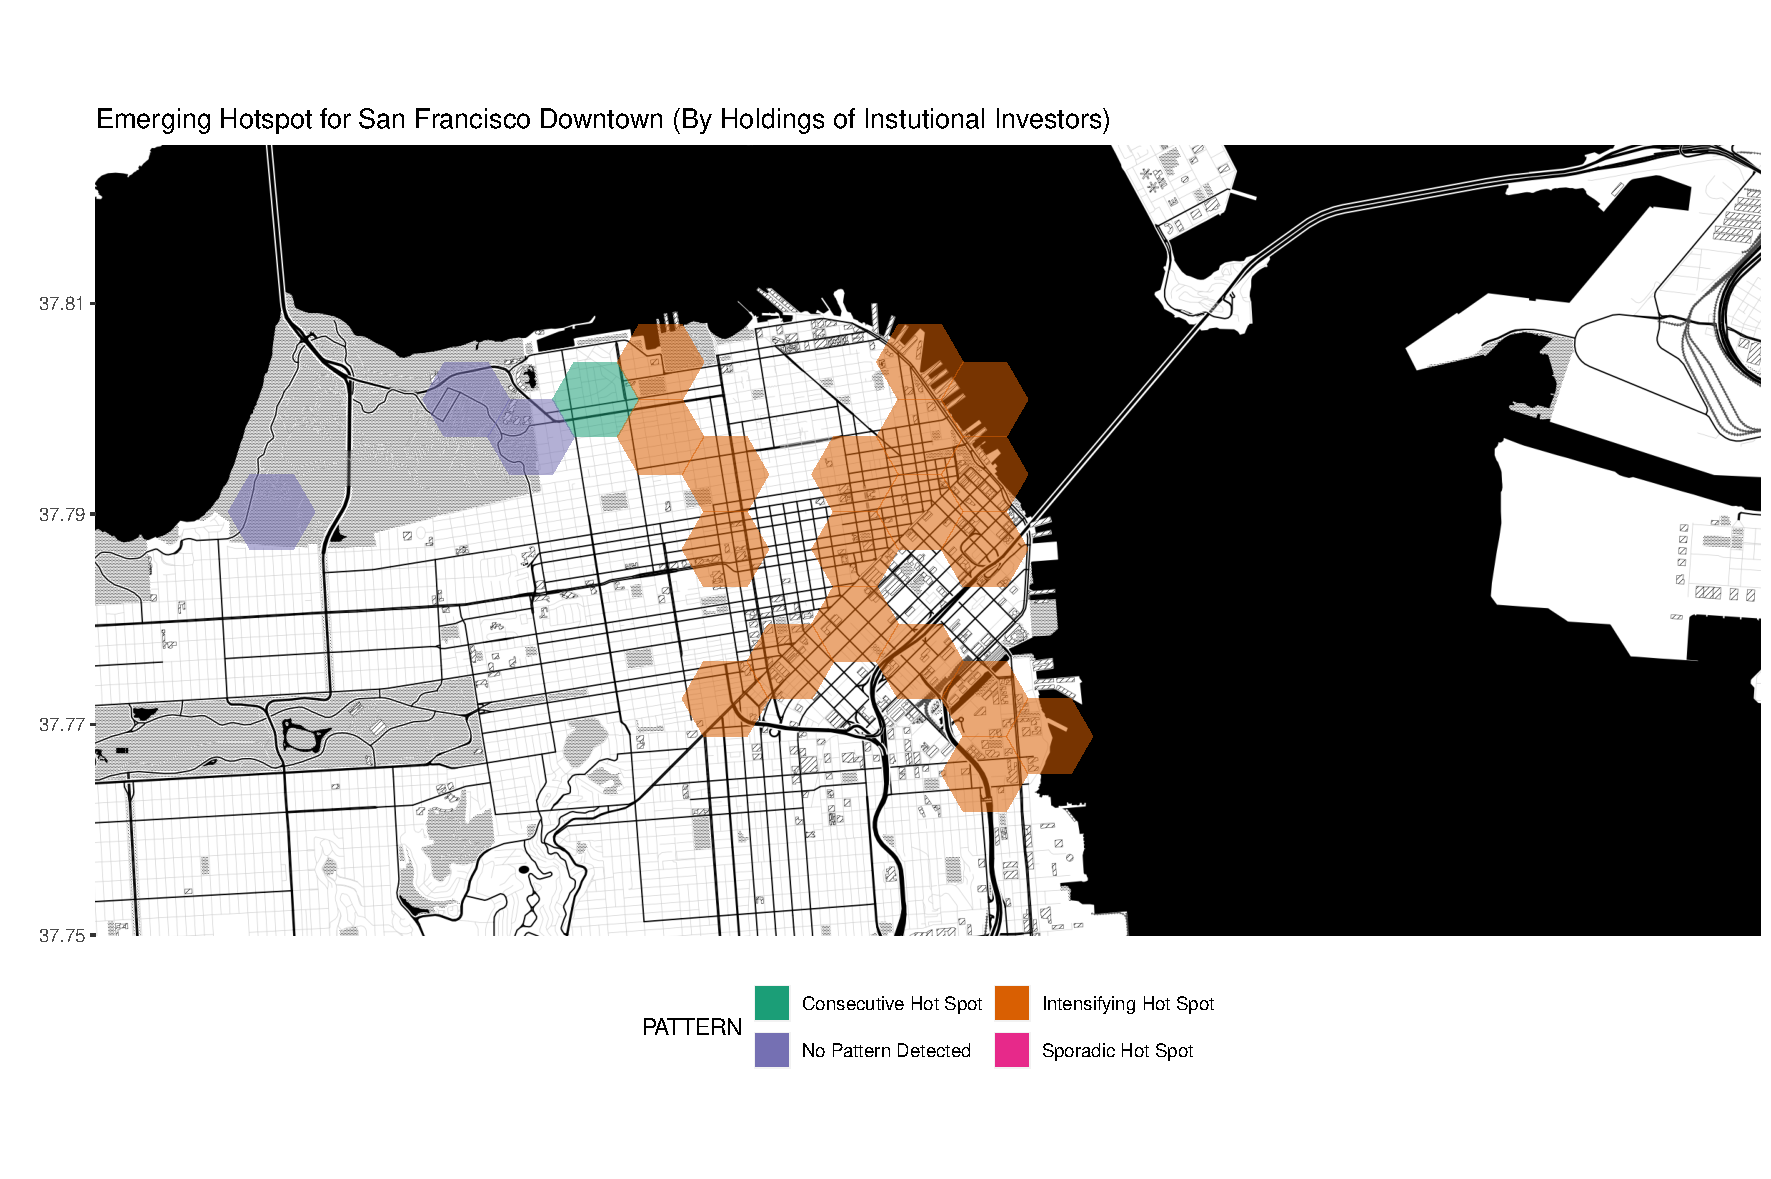
\includegraphics[width=1\linewidth]{Figures/ChapterIV/SF_Money_EH_Downtown}
	\caption[Emerging Hot Spot Analysis of Funds Under Management for Downtown San Francisco 2013-2018]{Emerging hot spot analysis of funds under management for downtown San Francisco for period June 2013 to December 2018}
	\label{fig:SFnmoneyhotspot_Downtown}
\end{figure}


\begin{figure}
	\centering
	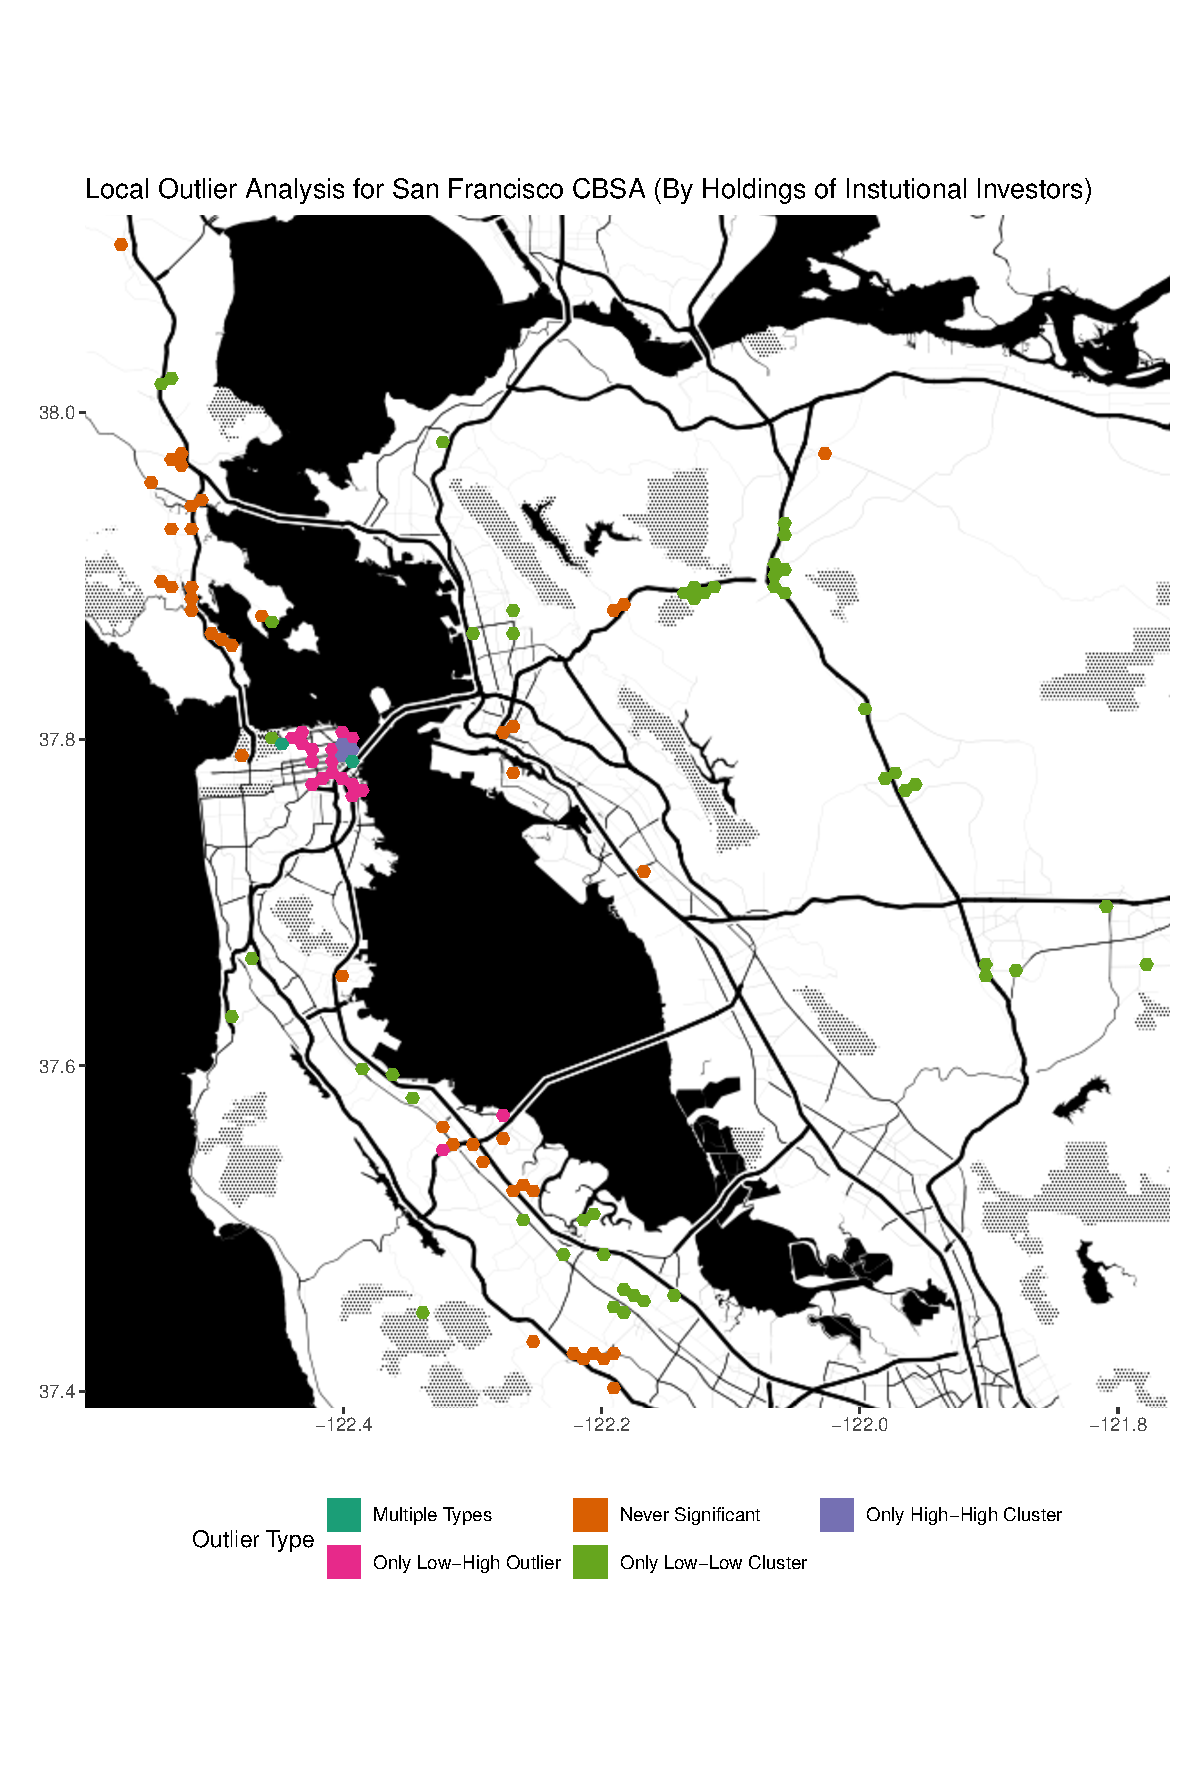
\includegraphics[width=1\linewidth]{Figures/ChapterIV/SF_Money_LO}
	\caption[San Francisco CBSA Local Outlier Analysis - Funds Under Management 2013-2018]{San Francisco local outlier analysis - funds under management}
	\label{fig:SFlocaloutlier}
\end{figure}

\begin{figure}
	\centering
	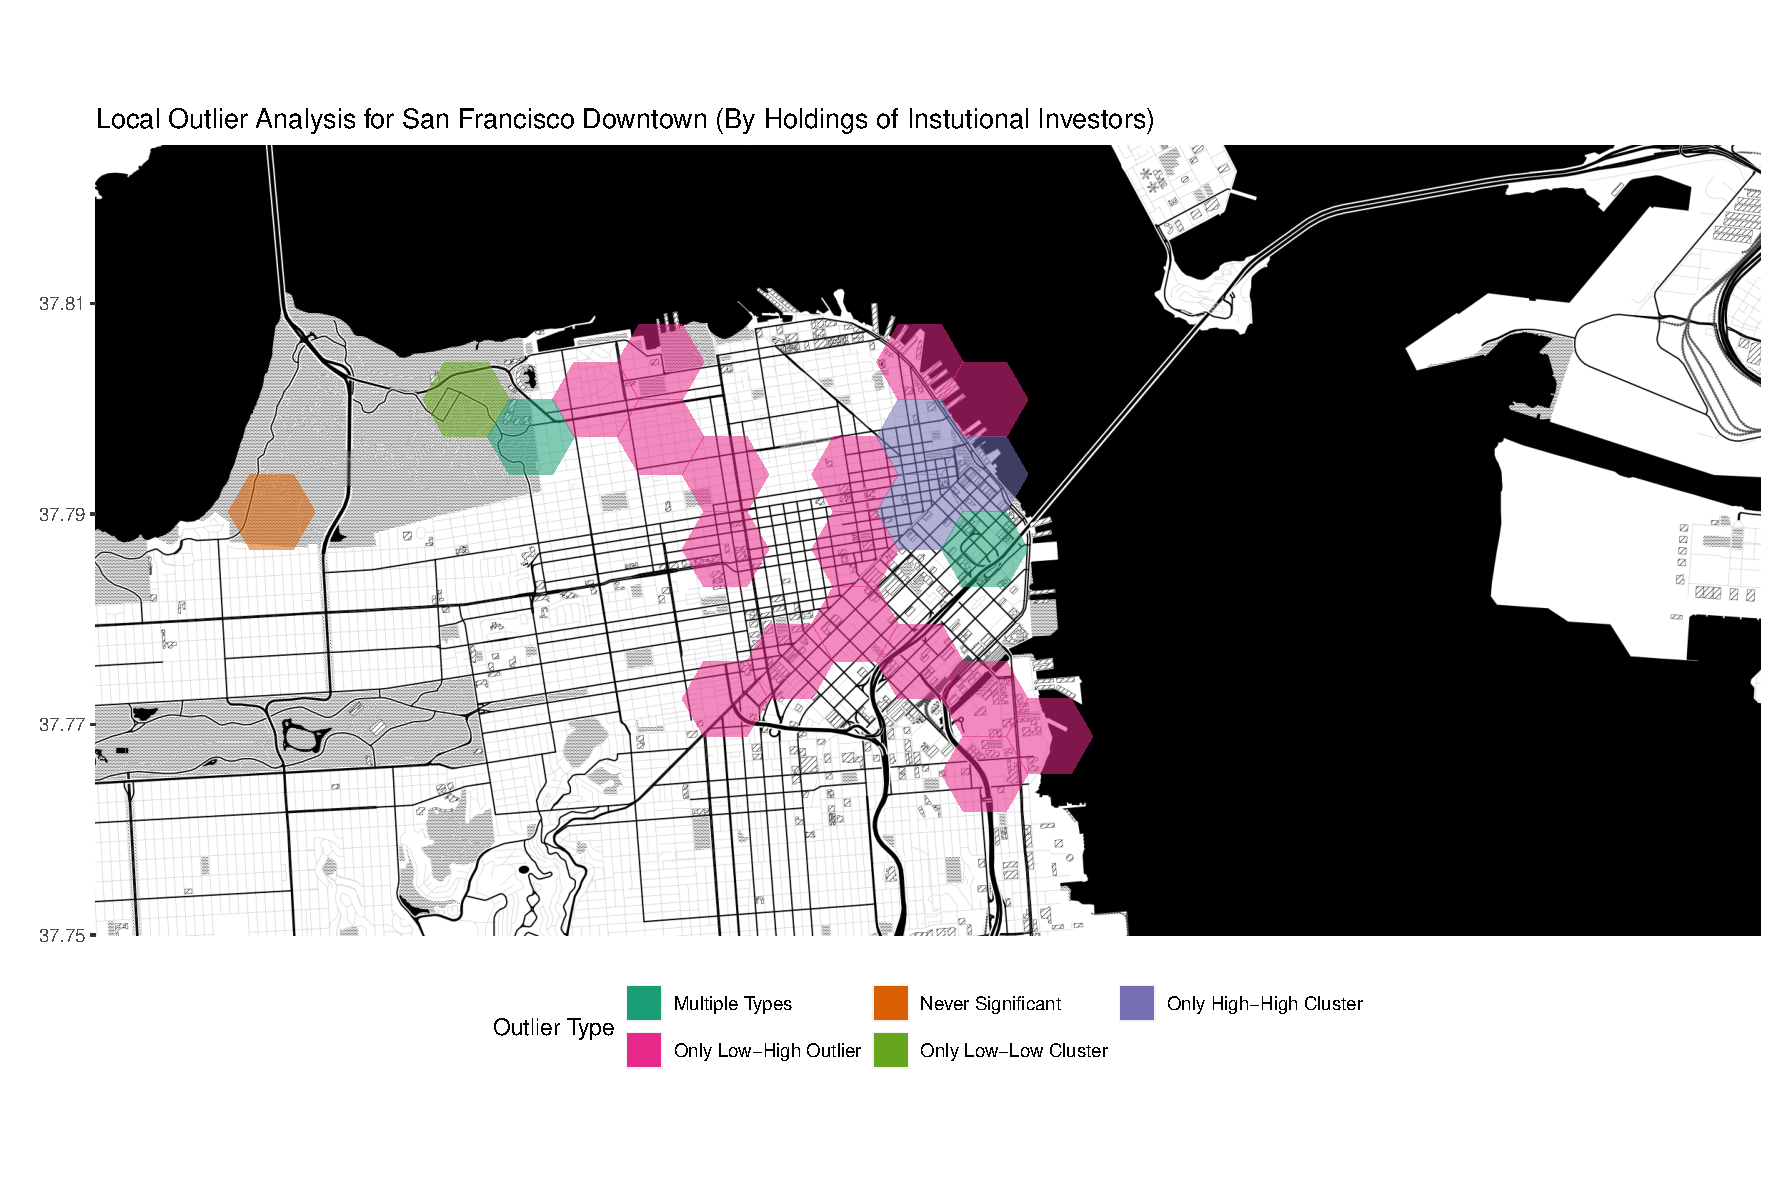
\includegraphics[width=1\linewidth]{Figures/ChapterIV/SF_Money_LO_Downtown}
	\caption[Downtown San Francisco Local Outlier Analysis - Funds Under Management 2013-2018]{Downtown San Francisco local outlier analysis - funds under management}
	\label{fig:SFlocaloutlier_Downtown}
\end{figure}
\section{Conclusion}	


When looking at the Continental United States, it appears that institutional investors are not evenly distributed across its vast surface.  As a matter of fact, other than a few outlying homesteads of institutional investors located in State capitals, most of the investors are located in the major metro areas of Boston, Chicago, Los Angeles, New York and San Francisco.  While one might be tempted to think that this is merely a collection of large US metro areas, the absence of population rich regions such as Dallas-Fort Worth, Houston, Philadelphia, Washington DC, Miami and Atlanta from the ranks of top cities is reassuring that the top 5 cities isn't simply a replication of XKCD Comic 1138 (Figure \ref{fig:heatmapxkcd}) using institutional investors rather than subscribers to Martha Stewart. 

Across these five cities, institutional investors exhibit a strong propensity to cluster, and more often than not these clusters are located in the downtown cores of cities.  Even with Los Angeles lack of a highly developed CBD for a city of it's size, its sprawling nature and deliberately decentralized history, the  existence of investor clusters somewhat pushes back against Graves's assertion that the benefits of co-location in an urban core were more than offset by the ever increasing cost of rents, and that investors of the future might seek more peripheral locations \citep{Graves2003}.   

That being said, one should not forget that identifying clusters can be problematic.  It is possible that new firms showing up on the periphery of a metro area's suburban spaces might not have the required density to show up as a cluster, even as the total ratio between CBD and suburbs may tilt evermore into the suburban office park's favour.  This is probably the most likely explanation for reconciling this chapter with Chapter \ref{ChapterIIIb}.  There are some hints at suburban centres being centres of clustering, notably the Route 128 in Boston, Evenston and Highland Park in Chicago, Irvine CA, and Walnut Creek in San Francisco.  However, it should be noted that these areas have a historically smaller bankroll than the investors that tend to aggregate into CBD, suggesting that there might be a size threshold where being in the CBD becomes more worthwhile than in suburban office parks.  

The buyer's remorse over choosing low land costs over a central location can been seen in the saga of the Swiss bank UBS.  This Swiss-headquartered multinational bank was attracted by Stamford Connecticut's low land prices and generous tax incentives.  However, this out of the way location became a severe hindrance in attracting top tier talent from New York's financial sector due to long commutes, as well as chronic difficulties in meeting with Manhattan-based clients \citep{NYT_2011}.    
